\documentclass[twoside]{book}

% Packages required by doxygen
\usepackage{fixltx2e}
\usepackage{calc}
\usepackage{doxygen}
\usepackage[export]{adjustbox} % also loads graphicx
\usepackage{graphicx}
\usepackage[utf8]{inputenc}
\usepackage{makeidx}
\usepackage{multicol}
\usepackage{multirow}
\PassOptionsToPackage{warn}{textcomp}
\usepackage{textcomp}
\usepackage[nointegrals]{wasysym}
\usepackage[table]{xcolor}

% Font selection
\usepackage[T1]{fontenc}
\usepackage[scaled=.90]{helvet}
\usepackage{courier}
\usepackage{amssymb}
\usepackage{sectsty}
\renewcommand{\familydefault}{\sfdefault}
\allsectionsfont{%
  \fontseries{bc}\selectfont%
  \color{darkgray}%
}
\renewcommand{\DoxyLabelFont}{%
  \fontseries{bc}\selectfont%
  \color{darkgray}%
}
\newcommand{\+}{\discretionary{\mbox{\scriptsize$\hookleftarrow$}}{}{}}

% Page & text layout
\usepackage{geometry}
\geometry{%
  a4paper,%
  top=2.5cm,%
  bottom=2.5cm,%
  left=2.5cm,%
  right=2.5cm%
}
\tolerance=750
\hfuzz=15pt
\hbadness=750
\setlength{\emergencystretch}{15pt}
\setlength{\parindent}{0cm}
\setlength{\parskip}{0.2cm}
\makeatletter
\renewcommand{\paragraph}{%
  \@startsection{paragraph}{4}{0ex}{-1.0ex}{1.0ex}{%
    \normalfont\normalsize\bfseries\SS@parafont%
  }%
}
\renewcommand{\subparagraph}{%
  \@startsection{subparagraph}{5}{0ex}{-1.0ex}{1.0ex}{%
    \normalfont\normalsize\bfseries\SS@subparafont%
  }%
}
\makeatother

% Headers & footers
\usepackage{fancyhdr}
\pagestyle{fancyplain}
\fancyhead[LE]{\fancyplain{}{\bfseries\thepage}}
\fancyhead[CE]{\fancyplain{}{}}
\fancyhead[RE]{\fancyplain{}{\bfseries\leftmark}}
\fancyhead[LO]{\fancyplain{}{\bfseries\rightmark}}
\fancyhead[CO]{\fancyplain{}{}}
\fancyhead[RO]{\fancyplain{}{\bfseries\thepage}}
\fancyfoot[LE]{\fancyplain{}{}}
\fancyfoot[CE]{\fancyplain{}{}}
\fancyfoot[RE]{\fancyplain{}{\bfseries\scriptsize Generated on Thu Jan 1 2015 22\+:36\+:22 for Snowflake by Doxygen }}
\fancyfoot[LO]{\fancyplain{}{\bfseries\scriptsize Generated on Thu Jan 1 2015 22\+:36\+:22 for Snowflake by Doxygen }}
\fancyfoot[CO]{\fancyplain{}{}}
\fancyfoot[RO]{\fancyplain{}{}}
\renewcommand{\footrulewidth}{0.4pt}
\renewcommand{\chaptermark}[1]{%
  \markboth{#1}{}%
}
\renewcommand{\sectionmark}[1]{%
  \markright{\thesection\ #1}%
}

% Indices & bibliography
\usepackage{natbib}
\usepackage[titles]{tocloft}
\setcounter{tocdepth}{3}
\setcounter{secnumdepth}{5}
\makeindex

% Hyperlinks (required, but should be loaded last)
\usepackage{ifpdf}
\ifpdf
  \usepackage[pdftex,pagebackref=true]{hyperref}
\else
  \usepackage[ps2pdf,pagebackref=true]{hyperref}
\fi
\hypersetup{%
  colorlinks=true,%
  linkcolor=blue,%
  citecolor=blue,%
  unicode%
}

% Custom commands
\newcommand{\clearemptydoublepage}{%
  \newpage{\pagestyle{empty}\cleardoublepage}%
}


%===== C O N T E N T S =====

\begin{document}

% Titlepage & ToC
\hypersetup{pageanchor=false,
             bookmarks=true,
             bookmarksnumbered=true,
             pdfencoding=unicode
            }
\pagenumbering{roman}
\begin{titlepage}
\vspace*{7cm}
\begin{center}%
{\Large Snowflake \\[1ex]\large api-\/pre-\/alpha }\\
\vspace*{1cm}
{\large Generated by Doxygen 1.8.9}\\
\vspace*{0.5cm}
{\small Thu Jan 1 2015 22:36:22}\\
\end{center}
\end{titlepage}
\clearemptydoublepage
\tableofcontents
\clearemptydoublepage
\pagenumbering{arabic}
\hypersetup{pageanchor=true}

%--- Begin generated contents ---
\chapter{Namespace Index}
\section{Namespace List}
Here is a list of all documented namespaces with brief descriptions\+:\begin{DoxyCompactList}
\item\contentsline{section}{\hyperlink{namespace_snowflake}{Snowflake} }{\pageref{namespace_snowflake}}{}
\item\contentsline{section}{\hyperlink{namespace_snowflake_1_1_ajax}{Snowflake.\+Ajax} }{\pageref{namespace_snowflake_1_1_ajax}}{}
\item\contentsline{section}{\hyperlink{namespace_snowflake_1_1_constants}{Snowflake.\+Constants} }{\pageref{namespace_snowflake_1_1_constants}}{}
\item\contentsline{section}{\hyperlink{namespace_snowflake_1_1_constants_1_1_plugin}{Snowflake.\+Constants.\+Plugin} }{\pageref{namespace_snowflake_1_1_constants_1_1_plugin}}{}
\item\contentsline{section}{\hyperlink{namespace_snowflake_1_1_controller}{Snowflake.\+Controller} }{\pageref{namespace_snowflake_1_1_controller}}{}
\item\contentsline{section}{\hyperlink{namespace_snowflake_1_1_emulator}{Snowflake.\+Emulator} }{\pageref{namespace_snowflake_1_1_emulator}}{}
\item\contentsline{section}{\hyperlink{namespace_snowflake_1_1_emulator_1_1_configuration}{Snowflake.\+Emulator.\+Configuration} }{\pageref{namespace_snowflake_1_1_emulator_1_1_configuration}}{}
\item\contentsline{section}{\hyperlink{namespace_snowflake_1_1_emulator_1_1_input}{Snowflake.\+Emulator.\+Input} }{\pageref{namespace_snowflake_1_1_emulator_1_1_input}}{}
\item\contentsline{section}{\hyperlink{namespace_snowflake_1_1_emulator_1_1_input_1_1_constants}{Snowflake.\+Emulator.\+Input.\+Constants} }{\pageref{namespace_snowflake_1_1_emulator_1_1_input_1_1_constants}}{}
\item\contentsline{section}{\hyperlink{namespace_snowflake_1_1_events}{Snowflake.\+Events} }{\pageref{namespace_snowflake_1_1_events}}{}
\item\contentsline{section}{\hyperlink{namespace_snowflake_1_1_events_1_1_core_events}{Snowflake.\+Events.\+Core\+Events} }{\pageref{namespace_snowflake_1_1_events_1_1_core_events}}{}
\item\contentsline{section}{\hyperlink{namespace_snowflake_1_1_game}{Snowflake.\+Game} }{\pageref{namespace_snowflake_1_1_game}}{}
\item\contentsline{section}{\hyperlink{namespace_snowflake_1_1_identifier}{Snowflake.\+Identifier} }{\pageref{namespace_snowflake_1_1_identifier}}{}
\item\contentsline{section}{\hyperlink{namespace_snowflake_1_1_information}{Snowflake.\+Information} }{\pageref{namespace_snowflake_1_1_information}}{}
\item\contentsline{section}{\hyperlink{namespace_snowflake_1_1_information_1_1_media_store}{Snowflake.\+Information.\+Media\+Store} }{\pageref{namespace_snowflake_1_1_information_1_1_media_store}}{}
\item\contentsline{section}{\hyperlink{namespace_snowflake_1_1_platform}{Snowflake.\+Platform} }{\pageref{namespace_snowflake_1_1_platform}}{}
\item\contentsline{section}{\hyperlink{namespace_snowflake_1_1_plugin}{Snowflake.\+Plugin} }{\pageref{namespace_snowflake_1_1_plugin}}{}
\item\contentsline{section}{\hyperlink{namespace_snowflake_1_1_scraper}{Snowflake.\+Scraper} }{\pageref{namespace_snowflake_1_1_scraper}}{}
\item\contentsline{section}{\hyperlink{namespace_snowflake_1_1_service}{Snowflake.\+Service} }{\pageref{namespace_snowflake_1_1_service}}{}
\item\contentsline{section}{\hyperlink{namespace_snowflake_1_1_service_1_1_http_server}{Snowflake.\+Service.\+Http\+Server} }{\pageref{namespace_snowflake_1_1_service_1_1_http_server}}{}
\item\contentsline{section}{\hyperlink{namespace_snowflake_1_1_service_1_1_manager}{Snowflake.\+Service.\+Manager} }{\pageref{namespace_snowflake_1_1_service_1_1_manager}}{}
\item\contentsline{section}{\hyperlink{namespace_snowflake_1_1_utility}{Snowflake.\+Utility} }{\pageref{namespace_snowflake_1_1_utility}}{}
\end{DoxyCompactList}

\chapter{Hierarchical Index}
\section{Class Hierarchy}
This inheritance list is sorted roughly, but not completely, alphabetically\+:\begin{DoxyCompactList}
\item Attribute\begin{DoxyCompactList}
\item \contentsline{section}{Snowflake.\+Ajax.\+Ajax\+Method\+Attribute}{\pageref{class_snowflake_1_1_ajax_1_1_ajax_method_attribute}}{}
\end{DoxyCompactList}
\item \contentsline{section}{Snowflake.\+Utility.\+Base\+Database}{\pageref{class_snowflake_1_1_utility_1_1_base_database}}{}
\item Event\+Args\begin{DoxyCompactList}
\item \contentsline{section}{Snowflake.\+Events.\+Core\+Events.\+Plugin\+Manager\+Loaded\+Event\+Args}{\pageref{class_snowflake_1_1_events_1_1_core_events_1_1_plugin_manager_loaded_event_args}}{}
\end{DoxyCompactList}
\item Hash\+Algorithm\begin{DoxyCompactList}
\item \contentsline{section}{Snowflake.\+Utility.\+Crc32}{\pageref{class_snowflake_1_1_utility_1_1_crc32}}{}
\end{DoxyCompactList}
\item \contentsline{section}{Snowflake.\+Service.\+Http\+Server.\+I\+Base\+Http\+Server}{\pageref{interface_snowflake_1_1_service_1_1_http_server_1_1_i_base_http_server}}{}
\begin{DoxyCompactList}
\item \contentsline{section}{Snowflake.\+Service.\+Http\+Server.\+Base\+Http\+Server}{\pageref{class_snowflake_1_1_service_1_1_http_server_1_1_base_http_server}}{}
\end{DoxyCompactList}
\item \contentsline{section}{Snowflake.\+Plugin.\+I\+Base\+Plugin}{\pageref{interface_snowflake_1_1_plugin_1_1_i_base_plugin}}{}
\begin{DoxyCompactList}
\item \contentsline{section}{Snowflake.\+Ajax.\+I\+Base\+Ajax\+Namespace}{\pageref{interface_snowflake_1_1_ajax_1_1_i_base_ajax_namespace}}{}
\begin{DoxyCompactList}
\item \contentsline{section}{Snowflake.\+Ajax.\+Base\+Ajax\+Namespace}{\pageref{class_snowflake_1_1_ajax_1_1_base_ajax_namespace}}{}
\end{DoxyCompactList}
\item \contentsline{section}{Snowflake.\+Emulator.\+I\+Emulator\+Bridge}{\pageref{interface_snowflake_1_1_emulator_1_1_i_emulator_bridge}}{}
\begin{DoxyCompactList}
\item \contentsline{section}{Snowflake.\+Emulator.\+Emulator\+Bridge}{\pageref{class_snowflake_1_1_emulator_1_1_emulator_bridge}}{}
\end{DoxyCompactList}
\item \contentsline{section}{Snowflake.\+Identifier.\+I\+Identifier}{\pageref{interface_snowflake_1_1_identifier_1_1_i_identifier}}{}
\item \contentsline{section}{Snowflake.\+Plugin.\+Base\+Plugin}{\pageref{class_snowflake_1_1_plugin_1_1_base_plugin}}{}
\begin{DoxyCompactList}
\item \contentsline{section}{Snowflake.\+Ajax.\+Base\+Ajax\+Namespace}{\pageref{class_snowflake_1_1_ajax_1_1_base_ajax_namespace}}{}
\item \contentsline{section}{Snowflake.\+Emulator.\+Emulator\+Bridge}{\pageref{class_snowflake_1_1_emulator_1_1_emulator_bridge}}{}
\item \contentsline{section}{Snowflake.\+Scraper.\+Base\+Scraper}{\pageref{class_snowflake_1_1_scraper_1_1_base_scraper}}{}
\end{DoxyCompactList}
\item \contentsline{section}{Snowflake.\+Plugin.\+I\+General\+Plugin}{\pageref{interface_snowflake_1_1_plugin_1_1_i_general_plugin}}{}
\item \contentsline{section}{Snowflake.\+Scraper.\+I\+Scraper}{\pageref{interface_snowflake_1_1_scraper_1_1_i_scraper}}{}
\begin{DoxyCompactList}
\item \contentsline{section}{Snowflake.\+Scraper.\+Base\+Scraper}{\pageref{class_snowflake_1_1_scraper_1_1_base_scraper}}{}
\end{DoxyCompactList}
\end{DoxyCompactList}
\item \contentsline{section}{Snowflake.\+Emulator.\+Configuration.\+I\+Boolean\+Mapping}{\pageref{interface_snowflake_1_1_emulator_1_1_configuration_1_1_i_boolean_mapping}}{}
\item \contentsline{section}{Snowflake.\+Emulator.\+Configuration.\+I\+Configuration\+Entry}{\pageref{interface_snowflake_1_1_emulator_1_1_configuration_1_1_i_configuration_entry}}{}
\item \contentsline{section}{Snowflake.\+Emulator.\+Configuration.\+I\+Configuration\+Flag}{\pageref{interface_snowflake_1_1_emulator_1_1_configuration_1_1_i_configuration_flag}}{}
\item \contentsline{section}{Snowflake.\+Emulator.\+Configuration.\+I\+Configuration\+Flag\+Database}{\pageref{interface_snowflake_1_1_emulator_1_1_configuration_1_1_i_configuration_flag_database}}{}
\item \contentsline{section}{Snowflake.\+Emulator.\+Configuration.\+I\+Configuration\+Profile}{\pageref{interface_snowflake_1_1_emulator_1_1_configuration_1_1_i_configuration_profile}}{}
\item \contentsline{section}{Snowflake.\+Emulator.\+Configuration.\+I\+Configuration\+Store}{\pageref{interface_snowflake_1_1_emulator_1_1_configuration_1_1_i_configuration_store}}{}
\item \contentsline{section}{Snowflake.\+Emulator.\+Configuration.\+I\+Configuration\+Template}{\pageref{interface_snowflake_1_1_emulator_1_1_configuration_1_1_i_configuration_template}}{}
\item \contentsline{section}{Snowflake.\+Controller.\+I\+Controller\+Definition}{\pageref{interface_snowflake_1_1_controller_1_1_i_controller_definition}}{}
\item \contentsline{section}{Snowflake.\+Controller.\+I\+Controller\+Input}{\pageref{interface_snowflake_1_1_controller_1_1_i_controller_input}}{}
\item \contentsline{section}{Snowflake.\+Emulator.\+Input.\+I\+Controller\+Mapping}{\pageref{interface_snowflake_1_1_emulator_1_1_input_1_1_i_controller_mapping}}{}
\item \contentsline{section}{Snowflake.\+Controller.\+I\+Controller\+Ports\+Database}{\pageref{interface_snowflake_1_1_controller_1_1_i_controller_ports_database}}{}
\item \contentsline{section}{Snowflake.\+Controller.\+I\+Controller\+Profile}{\pageref{interface_snowflake_1_1_controller_1_1_i_controller_profile}}{}
\item \contentsline{section}{Snowflake.\+Controller.\+I\+Controller\+Profile\+Database}{\pageref{interface_snowflake_1_1_controller_1_1_i_controller_profile_database}}{}
\item \contentsline{section}{Snowflake.\+Emulator.\+Input.\+I\+Controller\+Template}{\pageref{interface_snowflake_1_1_emulator_1_1_input_1_1_i_controller_template}}{}
\item \contentsline{section}{Snowflake.\+Service.\+I\+Core\+Service}{\pageref{interface_snowflake_1_1_service_1_1_i_core_service}}{}
\item I\+Dictionary\begin{DoxyCompactList}
\item \contentsline{section}{Snowflake.\+Utility.\+Bi\+Dictionary$<$ T\+First, T\+Second $>$}{\pageref{class_snowflake_1_1_utility_1_1_bi_dictionary}}{}
\item \contentsline{section}{Snowflake.\+Utility.\+Bi\+Dictionary$<$ T\+First, T\+Second $>$}{\pageref{class_snowflake_1_1_utility_1_1_bi_dictionary}}{}
\end{DoxyCompactList}
\item \contentsline{section}{Snowflake.\+Service.\+Manager.\+I\+Emulator\+Assemblies\+Manager}{\pageref{interface_snowflake_1_1_service_1_1_manager_1_1_i_emulator_assemblies_manager}}{}
\item \contentsline{section}{Snowflake.\+Emulator.\+I\+Emulator\+Assembly}{\pageref{interface_snowflake_1_1_emulator_1_1_i_emulator_assembly}}{}
\item \contentsline{section}{Snowflake.\+Game.\+I\+Game\+Database}{\pageref{interface_snowflake_1_1_game_1_1_i_game_database}}{}
\item \contentsline{section}{Snowflake.\+Scraper.\+I\+Game\+Images\+Result}{\pageref{interface_snowflake_1_1_scraper_1_1_i_game_images_result}}{}
\item \contentsline{section}{Snowflake.\+Emulator.\+Input.\+I\+Gamepad\+Mapping}{\pageref{interface_snowflake_1_1_emulator_1_1_input_1_1_i_gamepad_mapping}}{}
\item \contentsline{section}{Snowflake.\+Scraper.\+I\+Game\+Scrape\+Result}{\pageref{interface_snowflake_1_1_scraper_1_1_i_game_scrape_result}}{}
\item \contentsline{section}{Snowflake.\+Information.\+I\+Info}{\pageref{interface_snowflake_1_1_information_1_1_i_info}}{}
\begin{DoxyCompactList}
\item \contentsline{section}{Snowflake.\+Game.\+I\+Game\+Info}{\pageref{interface_snowflake_1_1_game_1_1_i_game_info}}{}
\item \contentsline{section}{Snowflake.\+Platform.\+I\+Platform\+Info}{\pageref{interface_snowflake_1_1_platform_1_1_i_platform_info}}{}
\end{DoxyCompactList}
\item \contentsline{section}{Snowflake.\+Emulator.\+Input.\+I\+Input\+Template}{\pageref{interface_snowflake_1_1_emulator_1_1_input_1_1_i_input_template}}{}
\item \contentsline{section}{Snowflake.\+Ajax.\+I\+J\+S\+Request}{\pageref{interface_snowflake_1_1_ajax_1_1_i_j_s_request}}{}
\item \contentsline{section}{Snowflake.\+Ajax.\+I\+J\+S\+Response}{\pageref{interface_snowflake_1_1_ajax_1_1_i_j_s_response}}{}
\item \contentsline{section}{Snowflake.\+Emulator.\+Input.\+I\+Keyboard\+Mapping}{\pageref{interface_snowflake_1_1_emulator_1_1_input_1_1_i_keyboard_mapping}}{}
\item \contentsline{section}{Snowflake.\+Service.\+Manager.\+I\+Loadable\+Manager}{\pageref{interface_snowflake_1_1_service_1_1_manager_1_1_i_loadable_manager}}{}
\begin{DoxyCompactList}
\item \contentsline{section}{Snowflake.\+Service.\+Manager.\+I\+Ajax\+Manager}{\pageref{interface_snowflake_1_1_service_1_1_manager_1_1_i_ajax_manager}}{}
\item \contentsline{section}{Snowflake.\+Service.\+Manager.\+I\+Plugin\+Manager}{\pageref{interface_snowflake_1_1_service_1_1_manager_1_1_i_plugin_manager}}{}
\end{DoxyCompactList}
\item \contentsline{section}{Snowflake.\+Information.\+Media\+Store.\+I\+Media\+Store}{\pageref{interface_snowflake_1_1_information_1_1_media_store_1_1_i_media_store}}{}
\item \contentsline{section}{Snowflake.\+Information.\+Media\+Store.\+I\+Media\+Store\+Section}{\pageref{interface_snowflake_1_1_information_1_1_media_store_1_1_i_media_store_section}}{}
\item \contentsline{section}{Snowflake.\+Platform.\+I\+Platform\+Defaults}{\pageref{interface_snowflake_1_1_platform_1_1_i_platform_defaults}}{}
\item \contentsline{section}{Snowflake.\+Plugin.\+I\+Plugin\+Configuration}{\pageref{interface_snowflake_1_1_plugin_1_1_i_plugin_configuration}}{}
\item I\+Read\+Only\+Dictionary\begin{DoxyCompactList}
\item \contentsline{section}{Snowflake.\+Utility.\+Bi\+Dictionary$<$ T\+First, T\+Second $>$}{\pageref{class_snowflake_1_1_utility_1_1_bi_dictionary}}{}
\end{DoxyCompactList}
\item \contentsline{section}{Snowflake.\+Service.\+I\+Scrape\+Service}{\pageref{interface_snowflake_1_1_service_1_1_i_scrape_service}}{}
\end{DoxyCompactList}

\chapter{Class Index}
\section{Class List}
Here are the classes, structs, unions and interfaces with brief descriptions\+:\begin{DoxyCompactList}
\item\contentsline{section}{\hyperlink{class_snowflake_1_1_ajax_1_1_ajax_method_attribute}{Snowflake.\+Ajax.\+Ajax\+Method\+Attribute} \\*Methods that will be exported in a Ajax\+Namespace plugin should be marked with this attribute Only methods in a \hyperlink{interface_snowflake_1_1_ajax_1_1_i_base_ajax_namespace}{Snowflake.\+Ajax.\+I\+Base\+Ajax\+Namespace} will be callable via \hyperlink{namespace_snowflake_1_1_ajax}{Ajax} }{\pageref{class_snowflake_1_1_ajax_1_1_ajax_method_attribute}}{}
\item\contentsline{section}{\hyperlink{class_snowflake_1_1_ajax_1_1_base_ajax_namespace}{Snowflake.\+Ajax.\+Base\+Ajax\+Namespace} \\*}{\pageref{class_snowflake_1_1_ajax_1_1_base_ajax_namespace}}{}
\item\contentsline{section}{\hyperlink{class_snowflake_1_1_utility_1_1_base_database}{Snowflake.\+Utility.\+Base\+Database} }{\pageref{class_snowflake_1_1_utility_1_1_base_database}}{}
\item\contentsline{section}{\hyperlink{class_snowflake_1_1_service_1_1_http_server_1_1_base_http_server}{Snowflake.\+Service.\+Http\+Server.\+Base\+Http\+Server} \\*}{\pageref{class_snowflake_1_1_service_1_1_http_server_1_1_base_http_server}}{}
\item\contentsline{section}{\hyperlink{class_snowflake_1_1_plugin_1_1_base_plugin}{Snowflake.\+Plugin.\+Base\+Plugin} }{\pageref{class_snowflake_1_1_plugin_1_1_base_plugin}}{}
\item\contentsline{section}{\hyperlink{class_snowflake_1_1_scraper_1_1_base_scraper}{Snowflake.\+Scraper.\+Base\+Scraper} }{\pageref{class_snowflake_1_1_scraper_1_1_base_scraper}}{}
\item\contentsline{section}{\hyperlink{class_snowflake_1_1_utility_1_1_bi_dictionary}{Snowflake.\+Utility.\+Bi\+Dictionary$<$ T\+First, T\+Second $>$} }{\pageref{class_snowflake_1_1_utility_1_1_bi_dictionary}}{}
\item\contentsline{section}{\hyperlink{class_snowflake_1_1_utility_1_1_crc32}{Snowflake.\+Utility.\+Crc32} \\*Implements a 32-\/bit C\+R\+C hash algorithm compatible with Zip etc. }{\pageref{class_snowflake_1_1_utility_1_1_crc32}}{}
\item\contentsline{section}{\hyperlink{class_snowflake_1_1_emulator_1_1_emulator_bridge}{Snowflake.\+Emulator.\+Emulator\+Bridge} }{\pageref{class_snowflake_1_1_emulator_1_1_emulator_bridge}}{}
\item\contentsline{section}{\hyperlink{interface_snowflake_1_1_service_1_1_manager_1_1_i_ajax_manager}{Snowflake.\+Service.\+Manager.\+I\+Ajax\+Manager} }{\pageref{interface_snowflake_1_1_service_1_1_manager_1_1_i_ajax_manager}}{}
\item\contentsline{section}{\hyperlink{interface_snowflake_1_1_ajax_1_1_i_base_ajax_namespace}{Snowflake.\+Ajax.\+I\+Base\+Ajax\+Namespace} \\*Methods to be callable via the Ajax\+Manager should be contained in an \hyperlink{interface_snowflake_1_1_ajax_1_1_i_base_ajax_namespace}{I\+Base\+Ajax\+Namespace} plugin. Snowflake.\+Ajax.\+Base\+Plugin for the implementation }{\pageref{interface_snowflake_1_1_ajax_1_1_i_base_ajax_namespace}}{}
\item\contentsline{section}{\hyperlink{interface_snowflake_1_1_service_1_1_http_server_1_1_i_base_http_server}{Snowflake.\+Service.\+Http\+Server.\+I\+Base\+Http\+Server} \\*Represents an \hyperlink{namespace_snowflake_1_1_service_1_1_http_server}{Http\+Server} that can be used to serve content. Snowflake.\+Server.\+Http\+Server.\+Process(\+Mono.\+Net.\+Http\+Listener\+Context) on how to implement the server loop }{\pageref{interface_snowflake_1_1_service_1_1_http_server_1_1_i_base_http_server}}{}
\item\contentsline{section}{\hyperlink{interface_snowflake_1_1_plugin_1_1_i_base_plugin}{Snowflake.\+Plugin.\+I\+Base\+Plugin} }{\pageref{interface_snowflake_1_1_plugin_1_1_i_base_plugin}}{}
\item\contentsline{section}{\hyperlink{interface_snowflake_1_1_emulator_1_1_configuration_1_1_i_boolean_mapping}{Snowflake.\+Emulator.\+Configuration.\+I\+Boolean\+Mapping} }{\pageref{interface_snowflake_1_1_emulator_1_1_configuration_1_1_i_boolean_mapping}}{}
\item\contentsline{section}{\hyperlink{interface_snowflake_1_1_emulator_1_1_configuration_1_1_i_configuration_entry}{Snowflake.\+Emulator.\+Configuration.\+I\+Configuration\+Entry} }{\pageref{interface_snowflake_1_1_emulator_1_1_configuration_1_1_i_configuration_entry}}{}
\item\contentsline{section}{\hyperlink{interface_snowflake_1_1_emulator_1_1_configuration_1_1_i_configuration_flag}{Snowflake.\+Emulator.\+Configuration.\+I\+Configuration\+Flag} }{\pageref{interface_snowflake_1_1_emulator_1_1_configuration_1_1_i_configuration_flag}}{}
\item\contentsline{section}{\hyperlink{interface_snowflake_1_1_emulator_1_1_configuration_1_1_i_configuration_flag_database}{Snowflake.\+Emulator.\+Configuration.\+I\+Configuration\+Flag\+Database} }{\pageref{interface_snowflake_1_1_emulator_1_1_configuration_1_1_i_configuration_flag_database}}{}
\item\contentsline{section}{\hyperlink{interface_snowflake_1_1_emulator_1_1_configuration_1_1_i_configuration_profile}{Snowflake.\+Emulator.\+Configuration.\+I\+Configuration\+Profile} }{\pageref{interface_snowflake_1_1_emulator_1_1_configuration_1_1_i_configuration_profile}}{}
\item\contentsline{section}{\hyperlink{interface_snowflake_1_1_emulator_1_1_configuration_1_1_i_configuration_store}{Snowflake.\+Emulator.\+Configuration.\+I\+Configuration\+Store} }{\pageref{interface_snowflake_1_1_emulator_1_1_configuration_1_1_i_configuration_store}}{}
\item\contentsline{section}{\hyperlink{interface_snowflake_1_1_emulator_1_1_configuration_1_1_i_configuration_template}{Snowflake.\+Emulator.\+Configuration.\+I\+Configuration\+Template} }{\pageref{interface_snowflake_1_1_emulator_1_1_configuration_1_1_i_configuration_template}}{}
\item\contentsline{section}{\hyperlink{interface_snowflake_1_1_controller_1_1_i_controller_definition}{Snowflake.\+Controller.\+I\+Controller\+Definition} \\*Represents a controller layout. Every input (button, triggers, analog sticks) is represeted as \hyperlink{interface_snowflake_1_1_controller_1_1_i_controller_input}{I\+Controller\+Input} \hyperlink{interface_snowflake_1_1_controller_1_1_i_controller_input}{Snowflake.\+Controller.\+I\+Controller\+Input} }{\pageref{interface_snowflake_1_1_controller_1_1_i_controller_definition}}{}
\item\contentsline{section}{\hyperlink{interface_snowflake_1_1_controller_1_1_i_controller_input}{Snowflake.\+Controller.\+I\+Controller\+Input} \\*Represents a single input on the controller. The recommended naming convention for Controller\+Inputs are For Buttons and Triggers\+: B\+T\+N\+\_\+ For D\+Pad\+: B\+T\+N\+\_\+\+D\+P\+A\+D\+\_\+ For movement of analog sticks, motion tracking and joysticks\+: A\+N\+A\+L\+O\+G\+\_\+ }{\pageref{interface_snowflake_1_1_controller_1_1_i_controller_input}}{}
\item\contentsline{section}{\hyperlink{interface_snowflake_1_1_emulator_1_1_input_1_1_i_controller_mapping}{Snowflake.\+Emulator.\+Input.\+I\+Controller\+Mapping} }{\pageref{interface_snowflake_1_1_emulator_1_1_input_1_1_i_controller_mapping}}{}
\item\contentsline{section}{\hyperlink{interface_snowflake_1_1_controller_1_1_i_controller_ports_database}{Snowflake.\+Controller.\+I\+Controller\+Ports\+Database} \\*This database stores which type of controller is to be used on which port. \hyperlink{namespace_snowflake}{Snowflake} supports up to 8 ports. It is recommended that when compiling controller profiles, the port number should indicate the slot of the controller profile to be used. Each port should correspond to a physical controller port on the console. Thus, player 1 should use the profile in slot 1 of the controller in port 1 Snowflake.\+Controller.\+I\+Controller\+Database }{\pageref{interface_snowflake_1_1_controller_1_1_i_controller_ports_database}}{}
\item\contentsline{section}{\hyperlink{interface_snowflake_1_1_controller_1_1_i_controller_profile}{Snowflake.\+Controller.\+I\+Controller\+Profile} \\*Represents a mapping from the controller definition to the gamepad or keyboard. Snowflake.\+Emulator.\+Input.\+Keyboard\+Mapping For \hyperlink{namespace_snowflake}{Snowflake}\textquotesingle{}s keyboard abstraction. \begin{DoxySeeAlso}{See also}
Snowflake.\+Emulator.\+Input.\+Gamepad\+Mapping


\end{DoxySeeAlso}
For \hyperlink{namespace_snowflake}{Snowflake}\textquotesingle{}s gamepad abstracion. }{\pageref{interface_snowflake_1_1_controller_1_1_i_controller_profile}}{}
\item\contentsline{section}{\hyperlink{interface_snowflake_1_1_controller_1_1_i_controller_profile_database}{Snowflake.\+Controller.\+I\+Controller\+Profile\+Database} \\*A database that holds the controller profile data for a certain slot. The database supports 1 to 8 slots or \textquotesingle{}controller\+Index\textquotesingle{}, \hyperlink{namespace_snowflake}{Snowflake} can only store up to 8 profiles for a controller. Every controller profile I\+D has their own table with all the inputs as a column prefixes with \textquotesingle{}I\+N\+P\+U\+T\+\_\+\textquotesingle{}. Profiles can be accessed once stored by the Controller\+I\+D of the controller definition the profile has mapped to, and the slot number. \hyperlink{interface_snowflake_1_1_controller_1_1_i_controller_profile}{Snowflake.\+Controller.\+I\+Controller\+Profile} \begin{DoxySeeAlso}{See also}
\hyperlink{interface_snowflake_1_1_controller_1_1_i_controller_definition}{Snowflake.\+Controller.\+I\+Controller\+Definition}


\end{DoxySeeAlso}
}{\pageref{interface_snowflake_1_1_controller_1_1_i_controller_profile_database}}{}
\item\contentsline{section}{\hyperlink{interface_snowflake_1_1_emulator_1_1_input_1_1_i_controller_template}{Snowflake.\+Emulator.\+Input.\+I\+Controller\+Template} }{\pageref{interface_snowflake_1_1_emulator_1_1_input_1_1_i_controller_template}}{}
\item\contentsline{section}{\hyperlink{interface_snowflake_1_1_service_1_1_i_core_service}{Snowflake.\+Service.\+I\+Core\+Service} }{\pageref{interface_snowflake_1_1_service_1_1_i_core_service}}{}
\item\contentsline{section}{\hyperlink{interface_snowflake_1_1_service_1_1_manager_1_1_i_emulator_assemblies_manager}{Snowflake.\+Service.\+Manager.\+I\+Emulator\+Assemblies\+Manager} }{\pageref{interface_snowflake_1_1_service_1_1_manager_1_1_i_emulator_assemblies_manager}}{}
\item\contentsline{section}{\hyperlink{interface_snowflake_1_1_emulator_1_1_i_emulator_assembly}{Snowflake.\+Emulator.\+I\+Emulator\+Assembly} }{\pageref{interface_snowflake_1_1_emulator_1_1_i_emulator_assembly}}{}
\item\contentsline{section}{\hyperlink{interface_snowflake_1_1_emulator_1_1_i_emulator_bridge}{Snowflake.\+Emulator.\+I\+Emulator\+Bridge} }{\pageref{interface_snowflake_1_1_emulator_1_1_i_emulator_bridge}}{}
\item\contentsline{section}{\hyperlink{interface_snowflake_1_1_game_1_1_i_game_database}{Snowflake.\+Game.\+I\+Game\+Database} \\*A database used to store game information }{\pageref{interface_snowflake_1_1_game_1_1_i_game_database}}{}
\item\contentsline{section}{\hyperlink{interface_snowflake_1_1_scraper_1_1_i_game_images_result}{Snowflake.\+Scraper.\+I\+Game\+Images\+Result} }{\pageref{interface_snowflake_1_1_scraper_1_1_i_game_images_result}}{}
\item\contentsline{section}{\hyperlink{interface_snowflake_1_1_game_1_1_i_game_info}{Snowflake.\+Game.\+I\+Game\+Info} \\*Represents a game with all it\textquotesingle{}s information }{\pageref{interface_snowflake_1_1_game_1_1_i_game_info}}{}
\item\contentsline{section}{\hyperlink{interface_snowflake_1_1_emulator_1_1_input_1_1_i_gamepad_mapping}{Snowflake.\+Emulator.\+Input.\+I\+Gamepad\+Mapping} }{\pageref{interface_snowflake_1_1_emulator_1_1_input_1_1_i_gamepad_mapping}}{}
\item\contentsline{section}{\hyperlink{interface_snowflake_1_1_scraper_1_1_i_game_scrape_result}{Snowflake.\+Scraper.\+I\+Game\+Scrape\+Result} }{\pageref{interface_snowflake_1_1_scraper_1_1_i_game_scrape_result}}{}
\item\contentsline{section}{\hyperlink{interface_snowflake_1_1_plugin_1_1_i_general_plugin}{Snowflake.\+Plugin.\+I\+General\+Plugin} }{\pageref{interface_snowflake_1_1_plugin_1_1_i_general_plugin}}{}
\item\contentsline{section}{\hyperlink{interface_snowflake_1_1_identifier_1_1_i_identifier}{Snowflake.\+Identifier.\+I\+Identifier} }{\pageref{interface_snowflake_1_1_identifier_1_1_i_identifier}}{}
\item\contentsline{section}{\hyperlink{interface_snowflake_1_1_information_1_1_i_info}{Snowflake.\+Information.\+I\+Info} \\*Represents an object that can have platform-\/relational information attached to it. \hyperlink{interface_snowflake_1_1_game_1_1_i_game_info}{Snowflake.\+Game.\+I\+Game\+Info} \begin{DoxySeeAlso}{See also}
\hyperlink{interface_snowflake_1_1_platform_1_1_i_platform_info}{Snowflake.\+Platform.\+I\+Platform\+Info}


\end{DoxySeeAlso}
}{\pageref{interface_snowflake_1_1_information_1_1_i_info}}{}
\item\contentsline{section}{\hyperlink{interface_snowflake_1_1_emulator_1_1_input_1_1_i_input_template}{Snowflake.\+Emulator.\+Input.\+I\+Input\+Template} }{\pageref{interface_snowflake_1_1_emulator_1_1_input_1_1_i_input_template}}{}
\item\contentsline{section}{\hyperlink{interface_snowflake_1_1_ajax_1_1_i_j_s_request}{Snowflake.\+Ajax.\+I\+J\+S\+Request} \\*Represents an \hyperlink{namespace_snowflake_1_1_ajax}{Ajax} Javascript Request }{\pageref{interface_snowflake_1_1_ajax_1_1_i_j_s_request}}{}
\item\contentsline{section}{\hyperlink{interface_snowflake_1_1_ajax_1_1_i_j_s_response}{Snowflake.\+Ajax.\+I\+J\+S\+Response} \\*Represents a Javascript (J\+S\+O\+N) response to an A\+J\+A\+X request }{\pageref{interface_snowflake_1_1_ajax_1_1_i_j_s_response}}{}
\item\contentsline{section}{\hyperlink{interface_snowflake_1_1_emulator_1_1_input_1_1_i_keyboard_mapping}{Snowflake.\+Emulator.\+Input.\+I\+Keyboard\+Mapping} }{\pageref{interface_snowflake_1_1_emulator_1_1_input_1_1_i_keyboard_mapping}}{}
\item\contentsline{section}{\hyperlink{interface_snowflake_1_1_service_1_1_manager_1_1_i_loadable_manager}{Snowflake.\+Service.\+Manager.\+I\+Loadable\+Manager} }{\pageref{interface_snowflake_1_1_service_1_1_manager_1_1_i_loadable_manager}}{}
\item\contentsline{section}{\hyperlink{interface_snowflake_1_1_information_1_1_media_store_1_1_i_media_store}{Snowflake.\+Information.\+Media\+Store.\+I\+Media\+Store} \\*Represents a mediastore that is able to store pieces of media for an \hyperlink{interface_snowflake_1_1_information_1_1_i_info}{I\+Info} }{\pageref{interface_snowflake_1_1_information_1_1_media_store_1_1_i_media_store}}{}
\item\contentsline{section}{\hyperlink{interface_snowflake_1_1_information_1_1_media_store_1_1_i_media_store_section}{Snowflake.\+Information.\+Media\+Store.\+I\+Media\+Store\+Section} \\*Represents a section in the mediastore. }{\pageref{interface_snowflake_1_1_information_1_1_media_store_1_1_i_media_store_section}}{}
\item\contentsline{section}{\hyperlink{interface_snowflake_1_1_platform_1_1_i_platform_defaults}{Snowflake.\+Platform.\+I\+Platform\+Defaults} }{\pageref{interface_snowflake_1_1_platform_1_1_i_platform_defaults}}{}
\item\contentsline{section}{\hyperlink{interface_snowflake_1_1_platform_1_1_i_platform_info}{Snowflake.\+Platform.\+I\+Platform\+Info} \\*Represents an emulated console or a platform in \hyperlink{namespace_snowflake}{Snowflake}. }{\pageref{interface_snowflake_1_1_platform_1_1_i_platform_info}}{}
\item\contentsline{section}{\hyperlink{interface_snowflake_1_1_plugin_1_1_i_plugin_configuration}{Snowflake.\+Plugin.\+I\+Plugin\+Configuration} }{\pageref{interface_snowflake_1_1_plugin_1_1_i_plugin_configuration}}{}
\item\contentsline{section}{\hyperlink{interface_snowflake_1_1_service_1_1_manager_1_1_i_plugin_manager}{Snowflake.\+Service.\+Manager.\+I\+Plugin\+Manager} }{\pageref{interface_snowflake_1_1_service_1_1_manager_1_1_i_plugin_manager}}{}
\item\contentsline{section}{\hyperlink{interface_snowflake_1_1_scraper_1_1_i_scraper}{Snowflake.\+Scraper.\+I\+Scraper} }{\pageref{interface_snowflake_1_1_scraper_1_1_i_scraper}}{}
\item\contentsline{section}{\hyperlink{interface_snowflake_1_1_service_1_1_i_scrape_service}{Snowflake.\+Service.\+I\+Scrape\+Service} }{\pageref{interface_snowflake_1_1_service_1_1_i_scrape_service}}{}
\item\contentsline{section}{\hyperlink{class_snowflake_1_1_events_1_1_core_events_1_1_plugin_manager_loaded_event_args}{Snowflake.\+Events.\+Core\+Events.\+Plugin\+Manager\+Loaded\+Event\+Args} }{\pageref{class_snowflake_1_1_events_1_1_core_events_1_1_plugin_manager_loaded_event_args}}{}
\end{DoxyCompactList}

\chapter{Namespace Documentation}
\hypertarget{namespace_snowflake}{}\section{Package Snowflake}
\label{namespace_snowflake}\index{Snowflake@{Snowflake}}
\subsection*{Namespaces}
\begin{DoxyCompactItemize}
\item 
package \hyperlink{namespace_snowflake_1_1_ajax}{Ajax}
\item 
package \hyperlink{namespace_snowflake_1_1_constants}{Constants}
\item 
package \hyperlink{namespace_snowflake_1_1_controller}{Controller}
\item 
package \hyperlink{namespace_snowflake_1_1_emulator}{Emulator}
\item 
package \hyperlink{namespace_snowflake_1_1_events}{Events}
\item 
package \hyperlink{namespace_snowflake_1_1_game}{Game}
\item 
package \hyperlink{namespace_snowflake_1_1_identifier}{Identifier}
\item 
package \hyperlink{namespace_snowflake_1_1_information}{Information}
\item 
package \hyperlink{namespace_snowflake_1_1_platform}{Platform}
\item 
package \hyperlink{namespace_snowflake_1_1_plugin}{Plugin}
\item 
package \hyperlink{namespace_snowflake_1_1_scraper}{Scraper}
\item 
package \hyperlink{namespace_snowflake_1_1_service}{Service}
\item 
package \hyperlink{namespace_snowflake_1_1_utility}{Utility}
\end{DoxyCompactItemize}

\hypertarget{namespace_snowflake_1_1_ajax}{}\section{Package Snowflake.\+Ajax}
\label{namespace_snowflake_1_1_ajax}\index{Snowflake.\+Ajax@{Snowflake.\+Ajax}}
\subsection*{Classes}
\begin{DoxyCompactItemize}
\item 
class \hyperlink{class_snowflake_1_1_ajax_1_1_ajax_method_attribute}{Ajax\+Method\+Attribute}
\begin{DoxyCompactList}\small\item\em Methods that will be exported in a Ajax\+Namespace plugin should be marked with this attribute Only methods in a \hyperlink{interface_snowflake_1_1_ajax_1_1_i_base_ajax_namespace}{Snowflake.\+Ajax.\+I\+Base\+Ajax\+Namespace} will be callable via \hyperlink{namespace_snowflake_1_1_ajax}{Ajax} \end{DoxyCompactList}\item 
class \hyperlink{class_snowflake_1_1_ajax_1_1_base_ajax_namespace}{Base\+Ajax\+Namespace}
\item 
interface \hyperlink{interface_snowflake_1_1_ajax_1_1_i_base_ajax_namespace}{I\+Base\+Ajax\+Namespace}
\begin{DoxyCompactList}\small\item\em Methods to be callable via the Ajax\+Manager should be contained in an \hyperlink{interface_snowflake_1_1_ajax_1_1_i_base_ajax_namespace}{I\+Base\+Ajax\+Namespace} plugin. Snowflake.\+Ajax.\+Base\+Plugin for the implementation \end{DoxyCompactList}\item 
interface \hyperlink{interface_snowflake_1_1_ajax_1_1_i_j_s_request}{I\+J\+S\+Request}
\begin{DoxyCompactList}\small\item\em Represents an \hyperlink{namespace_snowflake_1_1_ajax}{Ajax} Javascript Request \end{DoxyCompactList}\item 
interface \hyperlink{interface_snowflake_1_1_ajax_1_1_i_j_s_response}{I\+J\+S\+Response}
\begin{DoxyCompactList}\small\item\em Represents a Javascript (J\+S\+O\+N) response to an A\+J\+A\+X request \end{DoxyCompactList}\end{DoxyCompactItemize}

\hypertarget{namespace_snowflake_1_1_constants}{}\section{Package Snowflake.\+Constants}
\label{namespace_snowflake_1_1_constants}\index{Snowflake.\+Constants@{Snowflake.\+Constants}}
\subsection*{Namespaces}
\begin{DoxyCompactItemize}
\item 
package \hyperlink{namespace_snowflake_1_1_constants_1_1_plugin}{Plugin}
\end{DoxyCompactItemize}
\subsection*{Classes}
\begin{DoxyCompactItemize}
\item 
class {\bfseries Game\+Info\+Fields}
\item 
class {\bfseries Images\+Info\+Fields}
\end{DoxyCompactItemize}

\hypertarget{namespace_snowflake_1_1_constants_1_1_plugin}{}\section{Package Snowflake.\+Constants.\+Plugin}
\label{namespace_snowflake_1_1_constants_1_1_plugin}\index{Snowflake.\+Constants.\+Plugin@{Snowflake.\+Constants.\+Plugin}}
\subsection*{Classes}
\begin{DoxyCompactItemize}
\item 
class {\bfseries Plugin\+Info\+Fields}
\item 
class {\bfseries Scraper\+Info\+Fields}
\end{DoxyCompactItemize}

\hypertarget{namespace_snowflake_1_1_controller}{}\section{Package Snowflake.\+Controller}
\label{namespace_snowflake_1_1_controller}\index{Snowflake.\+Controller@{Snowflake.\+Controller}}
\subsection*{Classes}
\begin{DoxyCompactItemize}
\item 
interface \hyperlink{interface_snowflake_1_1_controller_1_1_i_controller_definition}{I\+Controller\+Definition}
\begin{DoxyCompactList}\small\item\em Represents a controller layout. Every input (button, triggers, analog sticks) is represeted as \hyperlink{interface_snowflake_1_1_controller_1_1_i_controller_input}{I\+Controller\+Input} \hyperlink{interface_snowflake_1_1_controller_1_1_i_controller_input}{Snowflake.\+Controller.\+I\+Controller\+Input} \end{DoxyCompactList}\item 
interface \hyperlink{interface_snowflake_1_1_controller_1_1_i_controller_input}{I\+Controller\+Input}
\begin{DoxyCompactList}\small\item\em Represents a single input on the controller. The recommended naming convention for Controller\+Inputs are For Buttons and Triggers\+: B\+T\+N\+\_\+ For D\+Pad\+: B\+T\+N\+\_\+\+D\+P\+A\+D\+\_\+ For movement of analog sticks, motion tracking and joysticks\+: A\+N\+A\+L\+O\+G\+\_\+ \end{DoxyCompactList}\item 
interface \hyperlink{interface_snowflake_1_1_controller_1_1_i_controller_ports_database}{I\+Controller\+Ports\+Database}
\begin{DoxyCompactList}\small\item\em This database stores which type of controller is to be used on which port. \hyperlink{namespace_snowflake}{Snowflake} supports up to 8 ports. It is recommended that when compiling controller profiles, the port number should indicate the slot of the controller profile to be used. Each port should correspond to a physical controller port on the console. Thus, player 1 should use the profile in slot 1 of the controller in port 1 Snowflake.\+Controller.\+I\+Controller\+Database \end{DoxyCompactList}\item 
interface \hyperlink{interface_snowflake_1_1_controller_1_1_i_controller_profile}{I\+Controller\+Profile}
\begin{DoxyCompactList}\small\item\em Represents a mapping from the controller definition to the gamepad or keyboard. Snowflake.\+Emulator.\+Input.\+Keyboard\+Mapping For \hyperlink{namespace_snowflake}{Snowflake}\textquotesingle{}s keyboard abstraction. \begin{DoxySeeAlso}{See also}
Snowflake.\+Emulator.\+Input.\+Gamepad\+Mapping


\end{DoxySeeAlso}
For \hyperlink{namespace_snowflake}{Snowflake}\textquotesingle{}s gamepad abstracion. \end{DoxyCompactList}\item 
interface \hyperlink{interface_snowflake_1_1_controller_1_1_i_controller_profile_database}{I\+Controller\+Profile\+Database}
\begin{DoxyCompactList}\small\item\em A database that holds the controller profile data for a certain slot. The database supports 1 to 8 slots or \textquotesingle{}controller\+Index\textquotesingle{}, \hyperlink{namespace_snowflake}{Snowflake} can only store up to 8 profiles for a controller. Every controller profile I\+D has their own table with all the inputs as a column prefixes with \textquotesingle{}I\+N\+P\+U\+T\+\_\+\textquotesingle{}. Profiles can be accessed once stored by the Controller\+I\+D of the controller definition the profile has mapped to, and the slot number. \hyperlink{interface_snowflake_1_1_controller_1_1_i_controller_profile}{Snowflake.\+Controller.\+I\+Controller\+Profile} \begin{DoxySeeAlso}{See also}
\hyperlink{interface_snowflake_1_1_controller_1_1_i_controller_definition}{Snowflake.\+Controller.\+I\+Controller\+Definition}


\end{DoxySeeAlso}
\end{DoxyCompactList}\end{DoxyCompactItemize}
\subsection*{Enumerations}
\begin{DoxyCompactItemize}
\item 
enum \hyperlink{namespace_snowflake_1_1_controller_af6896d98053b4f8f2d42c32c6fb05c96}{Controller\+Profile\+Type} \{ \hyperlink{namespace_snowflake_1_1_controller_af6896d98053b4f8f2d42c32c6fb05c96ae9f241ed90f10d7d5bd2db821e559948}{Controller\+Profile\+Type.\+G\+A\+M\+E\+P\+A\+D\+\_\+\+P\+R\+O\+F\+I\+L\+E}, 
\hyperlink{namespace_snowflake_1_1_controller_af6896d98053b4f8f2d42c32c6fb05c96ab8fca83ec4dcb034a3c1a31285bbc432}{Controller\+Profile\+Type.\+K\+E\+Y\+B\+O\+A\+R\+D\+\_\+\+P\+R\+O\+F\+I\+L\+E}, 
\hyperlink{namespace_snowflake_1_1_controller_af6896d98053b4f8f2d42c32c6fb05c96abb8d1b08d5f2d8121aa2d1f026297293}{Controller\+Profile\+Type.\+C\+U\+S\+T\+O\+M\+\_\+\+P\+R\+O\+F\+I\+L\+E}
 \}
\begin{DoxyCompactList}\small\item\em Types of Controller\+Profile \end{DoxyCompactList}\end{DoxyCompactItemize}


\subsection{Enumeration Type Documentation}
\hypertarget{namespace_snowflake_1_1_controller_af6896d98053b4f8f2d42c32c6fb05c96}{}\index{Snowflake\+::\+Controller@{Snowflake\+::\+Controller}!Controller\+Profile\+Type@{Controller\+Profile\+Type}}
\index{Controller\+Profile\+Type@{Controller\+Profile\+Type}!Snowflake\+::\+Controller@{Snowflake\+::\+Controller}}
\subsubsection[{Controller\+Profile\+Type}]{\setlength{\rightskip}{0pt plus 5cm}enum {\bf Snowflake.\+Controller.\+Controller\+Profile\+Type}}\label{namespace_snowflake_1_1_controller_af6896d98053b4f8f2d42c32c6fb05c96}


Types of Controller\+Profile 

\begin{Desc}
\item[Enumerator]\par
\begin{description}
\index{G\+A\+M\+E\+P\+A\+D\+\_\+\+P\+R\+O\+F\+I\+L\+E@{G\+A\+M\+E\+P\+A\+D\+\_\+\+P\+R\+O\+F\+I\+L\+E}!Snowflake\+::\+Controller@{Snowflake\+::\+Controller}}\index{Snowflake\+::\+Controller@{Snowflake\+::\+Controller}!G\+A\+M\+E\+P\+A\+D\+\_\+\+P\+R\+O\+F\+I\+L\+E@{G\+A\+M\+E\+P\+A\+D\+\_\+\+P\+R\+O\+F\+I\+L\+E}}\item[{\em 
\hypertarget{namespace_snowflake_1_1_controller_af6896d98053b4f8f2d42c32c6fb05c96ae9f241ed90f10d7d5bd2db821e559948}{}G\+A\+M\+E\+P\+A\+D\+\_\+\+P\+R\+O\+F\+I\+L\+E\label{namespace_snowflake_1_1_controller_af6896d98053b4f8f2d42c32c6fb05c96ae9f241ed90f10d7d5bd2db821e559948}
}]A profile that maps to a standard X\+Input-\/style gamepad \index{K\+E\+Y\+B\+O\+A\+R\+D\+\_\+\+P\+R\+O\+F\+I\+L\+E@{K\+E\+Y\+B\+O\+A\+R\+D\+\_\+\+P\+R\+O\+F\+I\+L\+E}!Snowflake\+::\+Controller@{Snowflake\+::\+Controller}}\index{Snowflake\+::\+Controller@{Snowflake\+::\+Controller}!K\+E\+Y\+B\+O\+A\+R\+D\+\_\+\+P\+R\+O\+F\+I\+L\+E@{K\+E\+Y\+B\+O\+A\+R\+D\+\_\+\+P\+R\+O\+F\+I\+L\+E}}\item[{\em 
\hypertarget{namespace_snowflake_1_1_controller_af6896d98053b4f8f2d42c32c6fb05c96ab8fca83ec4dcb034a3c1a31285bbc432}{}K\+E\+Y\+B\+O\+A\+R\+D\+\_\+\+P\+R\+O\+F\+I\+L\+E\label{namespace_snowflake_1_1_controller_af6896d98053b4f8f2d42c32c6fb05c96ab8fca83ec4dcb034a3c1a31285bbc432}
}]A profile that maps to a standard keyboard \index{C\+U\+S\+T\+O\+M\+\_\+\+P\+R\+O\+F\+I\+L\+E@{C\+U\+S\+T\+O\+M\+\_\+\+P\+R\+O\+F\+I\+L\+E}!Snowflake\+::\+Controller@{Snowflake\+::\+Controller}}\index{Snowflake\+::\+Controller@{Snowflake\+::\+Controller}!C\+U\+S\+T\+O\+M\+\_\+\+P\+R\+O\+F\+I\+L\+E@{C\+U\+S\+T\+O\+M\+\_\+\+P\+R\+O\+F\+I\+L\+E}}\item[{\em 
\hypertarget{namespace_snowflake_1_1_controller_af6896d98053b4f8f2d42c32c6fb05c96abb8d1b08d5f2d8121aa2d1f026297293}{}C\+U\+S\+T\+O\+M\+\_\+\+P\+R\+O\+F\+I\+L\+E\label{namespace_snowflake_1_1_controller_af6896d98053b4f8f2d42c32c6fb05c96abb8d1b08d5f2d8121aa2d1f026297293}
}]A custom (unknown) type of profile. A controller with type {\bfseries C\+U\+S\+T\+O\+M\+\_\+\+P\+R\+O\+F\+I\+L\+E} is unhandled, the \hyperlink{interface_snowflake_1_1_emulator_1_1_i_emulator_bridge}{Snowflake.\+Emulator.\+I\+Emulator\+Bridge} must handle this case manually\end{description}
\end{Desc}

\hypertarget{namespace_snowflake_1_1_emulator}{}\section{Package Snowflake.\+Emulator}
\label{namespace_snowflake_1_1_emulator}\index{Snowflake.\+Emulator@{Snowflake.\+Emulator}}
\subsection*{Namespaces}
\begin{DoxyCompactItemize}
\item 
package \hyperlink{namespace_snowflake_1_1_emulator_1_1_configuration}{Configuration}
\item 
package \hyperlink{namespace_snowflake_1_1_emulator_1_1_input}{Input}
\end{DoxyCompactItemize}
\subsection*{Classes}
\begin{DoxyCompactItemize}
\item 
class \hyperlink{class_snowflake_1_1_emulator_1_1_emulator_bridge}{Emulator\+Bridge}
\item 
interface \hyperlink{interface_snowflake_1_1_emulator_1_1_i_emulator_assembly}{I\+Emulator\+Assembly}
\item 
interface \hyperlink{interface_snowflake_1_1_emulator_1_1_i_emulator_bridge}{I\+Emulator\+Bridge}
\end{DoxyCompactItemize}
\subsection*{Enumerations}
\begin{DoxyCompactItemize}
\item 
\hypertarget{namespace_snowflake_1_1_emulator_a31029bdf1c1f4559664a26c486df1603}{}enum {\bfseries Emulator\+Assembly\+Type} \{ {\bfseries E\+M\+U\+L\+A\+T\+O\+R\+\_\+\+E\+X\+E\+C\+U\+T\+A\+B\+L\+E}, 
{\bfseries E\+M\+U\+L\+A\+T\+O\+R\+\_\+\+L\+I\+B\+R\+A\+R\+Y}, 
{\bfseries E\+M\+U\+L\+A\+T\+O\+R\+\_\+\+M\+I\+S\+C}
 \}\label{namespace_snowflake_1_1_emulator_a31029bdf1c1f4559664a26c486df1603}

\end{DoxyCompactItemize}

\hypertarget{namespace_snowflake_1_1_emulator_1_1_configuration}{}\section{Package Snowflake.\+Emulator.\+Configuration}
\label{namespace_snowflake_1_1_emulator_1_1_configuration}\index{Snowflake.\+Emulator.\+Configuration@{Snowflake.\+Emulator.\+Configuration}}
\subsection*{Classes}
\begin{DoxyCompactItemize}
\item 
interface \hyperlink{interface_snowflake_1_1_emulator_1_1_configuration_1_1_i_boolean_mapping}{I\+Boolean\+Mapping}
\item 
interface \hyperlink{interface_snowflake_1_1_emulator_1_1_configuration_1_1_i_configuration_entry}{I\+Configuration\+Entry}
\item 
interface \hyperlink{interface_snowflake_1_1_emulator_1_1_configuration_1_1_i_configuration_flag}{I\+Configuration\+Flag}
\item 
interface \hyperlink{interface_snowflake_1_1_emulator_1_1_configuration_1_1_i_configuration_flag_database}{I\+Configuration\+Flag\+Database}
\item 
interface \hyperlink{interface_snowflake_1_1_emulator_1_1_configuration_1_1_i_configuration_profile}{I\+Configuration\+Profile}
\item 
interface \hyperlink{interface_snowflake_1_1_emulator_1_1_configuration_1_1_i_configuration_store}{I\+Configuration\+Store}
\item 
interface \hyperlink{interface_snowflake_1_1_emulator_1_1_configuration_1_1_i_configuration_template}{I\+Configuration\+Template}
\end{DoxyCompactItemize}
\subsection*{Enumerations}
\begin{DoxyCompactItemize}
\item 
\hypertarget{namespace_snowflake_1_1_emulator_1_1_configuration_a2e92d84febdf23dc35b2ccdea8b599f2}{}enum {\bfseries Configuration\+Flag\+Types} \{ {\bfseries B\+O\+O\+L\+E\+A\+N\+\_\+\+F\+L\+A\+G}, 
{\bfseries I\+N\+T\+E\+G\+E\+R\+\_\+\+F\+L\+A\+G}, 
{\bfseries S\+E\+L\+E\+C\+T\+\_\+\+F\+L\+A\+G}
 \}\label{namespace_snowflake_1_1_emulator_1_1_configuration_a2e92d84febdf23dc35b2ccdea8b599f2}

\end{DoxyCompactItemize}

\hypertarget{namespace_snowflake_1_1_emulator_1_1_input}{}\section{Package Snowflake.\+Emulator.\+Input}
\label{namespace_snowflake_1_1_emulator_1_1_input}\index{Snowflake.\+Emulator.\+Input@{Snowflake.\+Emulator.\+Input}}
\subsection*{Namespaces}
\begin{DoxyCompactItemize}
\item 
package \hyperlink{namespace_snowflake_1_1_emulator_1_1_input_1_1_constants}{Constants}
\end{DoxyCompactItemize}
\subsection*{Classes}
\begin{DoxyCompactItemize}
\item 
interface \hyperlink{interface_snowflake_1_1_emulator_1_1_input_1_1_i_controller_mapping}{I\+Controller\+Mapping}
\item 
interface \hyperlink{interface_snowflake_1_1_emulator_1_1_input_1_1_i_controller_template}{I\+Controller\+Template}
\item 
interface \hyperlink{interface_snowflake_1_1_emulator_1_1_input_1_1_i_gamepad_mapping}{I\+Gamepad\+Mapping}
\item 
interface \hyperlink{interface_snowflake_1_1_emulator_1_1_input_1_1_i_input_template}{I\+Input\+Template}
\item 
interface \hyperlink{interface_snowflake_1_1_emulator_1_1_input_1_1_i_keyboard_mapping}{I\+Keyboard\+Mapping}
\end{DoxyCompactItemize}
\subsection*{Enumerations}
\begin{DoxyCompactItemize}
\item 
\hypertarget{namespace_snowflake_1_1_emulator_1_1_input_a11c378a2c1b47408ab41ad3d005d30db}{}enum {\bfseries Controller\+Mapping\+Type} \{ {\bfseries G\+A\+M\+E\+P\+A\+D\+\_\+\+M\+A\+P\+P\+I\+N\+G}, 
{\bfseries K\+E\+Y\+B\+O\+A\+R\+D\+\_\+\+M\+A\+P\+P\+I\+N\+G}
 \}\label{namespace_snowflake_1_1_emulator_1_1_input_a11c378a2c1b47408ab41ad3d005d30db}

\end{DoxyCompactItemize}

\hypertarget{namespace_snowflake_1_1_emulator_1_1_input_1_1_constants}{}\section{Package Snowflake.\+Emulator.\+Input.\+Constants}
\label{namespace_snowflake_1_1_emulator_1_1_input_1_1_constants}\index{Snowflake.\+Emulator.\+Input.\+Constants@{Snowflake.\+Emulator.\+Input.\+Constants}}
\subsection*{Classes}
\begin{DoxyCompactItemize}
\item 
class {\bfseries Gamepad\+Constants}
\item 
class {\bfseries Keyboard\+Constants}
\end{DoxyCompactItemize}

\hypertarget{namespace_snowflake_1_1_events}{}\section{Package Snowflake.\+Events}
\label{namespace_snowflake_1_1_events}\index{Snowflake.\+Events@{Snowflake.\+Events}}
\subsection*{Namespaces}
\begin{DoxyCompactItemize}
\item 
package \hyperlink{namespace_snowflake_1_1_events_1_1_core_events}{Core\+Events}
\end{DoxyCompactItemize}

\hypertarget{namespace_snowflake_1_1_events_1_1_core_events}{}\section{Package Snowflake.\+Events.\+Core\+Events}
\label{namespace_snowflake_1_1_events_1_1_core_events}\index{Snowflake.\+Events.\+Core\+Events@{Snowflake.\+Events.\+Core\+Events}}
\subsection*{Classes}
\begin{DoxyCompactItemize}
\item 
class \hyperlink{class_snowflake_1_1_events_1_1_core_events_1_1_plugin_manager_loaded_event_args}{Plugin\+Manager\+Loaded\+Event\+Args}
\end{DoxyCompactItemize}

\hypertarget{namespace_snowflake_1_1_game}{}\section{Package Snowflake.\+Game}
\label{namespace_snowflake_1_1_game}\index{Snowflake.\+Game@{Snowflake.\+Game}}
\subsection*{Classes}
\begin{DoxyCompactItemize}
\item 
interface \hyperlink{interface_snowflake_1_1_game_1_1_i_game_database}{I\+Game\+Database}
\begin{DoxyCompactList}\small\item\em A database used to store game information \end{DoxyCompactList}\item 
interface \hyperlink{interface_snowflake_1_1_game_1_1_i_game_info}{I\+Game\+Info}
\begin{DoxyCompactList}\small\item\em Represents a game with all it\textquotesingle{}s information \end{DoxyCompactList}\end{DoxyCompactItemize}

\hypertarget{namespace_snowflake_1_1_identifier}{}\section{Package Snowflake.\+Identifier}
\label{namespace_snowflake_1_1_identifier}\index{Snowflake.\+Identifier@{Snowflake.\+Identifier}}
\subsection*{Classes}
\begin{DoxyCompactItemize}
\item 
interface \hyperlink{interface_snowflake_1_1_identifier_1_1_i_identifier}{I\+Identifier}
\end{DoxyCompactItemize}

\hypertarget{namespace_snowflake_1_1_information}{}\section{Package Snowflake.\+Information}
\label{namespace_snowflake_1_1_information}\index{Snowflake.\+Information@{Snowflake.\+Information}}
\subsection*{Namespaces}
\begin{DoxyCompactItemize}
\item 
package \hyperlink{namespace_snowflake_1_1_information_1_1_media_store}{Media\+Store}
\end{DoxyCompactItemize}
\subsection*{Classes}
\begin{DoxyCompactItemize}
\item 
interface \hyperlink{interface_snowflake_1_1_information_1_1_i_info}{I\+Info}
\end{DoxyCompactItemize}

\hypertarget{namespace_snowflake_1_1_information_1_1_media_store}{}\section{Package Snowflake.\+Information.\+Media\+Store}
\label{namespace_snowflake_1_1_information_1_1_media_store}\index{Snowflake.\+Information.\+Media\+Store@{Snowflake.\+Information.\+Media\+Store}}
\subsection*{Classes}
\begin{DoxyCompactItemize}
\item 
interface \hyperlink{interface_snowflake_1_1_information_1_1_media_store_1_1_i_media_store}{I\+Media\+Store}
\item 
interface \hyperlink{interface_snowflake_1_1_information_1_1_media_store_1_1_i_media_store_section}{I\+Media\+Store\+Section}
\end{DoxyCompactItemize}

\hypertarget{namespace_snowflake_1_1_platform}{}\section{Package Snowflake.\+Platform}
\label{namespace_snowflake_1_1_platform}\index{Snowflake.\+Platform@{Snowflake.\+Platform}}
\subsection*{Classes}
\begin{DoxyCompactItemize}
\item 
interface \hyperlink{interface_snowflake_1_1_platform_1_1_i_platform_defaults}{I\+Platform\+Defaults}
\item 
interface \hyperlink{interface_snowflake_1_1_platform_1_1_i_platform_info}{I\+Platform\+Info}
\end{DoxyCompactItemize}

\hypertarget{namespace_snowflake_1_1_plugin}{}\section{Package Snowflake.\+Plugin}
\label{namespace_snowflake_1_1_plugin}\index{Snowflake.\+Plugin@{Snowflake.\+Plugin}}
\subsection*{Classes}
\begin{DoxyCompactItemize}
\item 
class \hyperlink{class_snowflake_1_1_plugin_1_1_base_plugin}{Base\+Plugin}
\item 
interface \hyperlink{interface_snowflake_1_1_plugin_1_1_i_base_plugin}{I\+Base\+Plugin}
\item 
interface \hyperlink{interface_snowflake_1_1_plugin_1_1_i_general_plugin}{I\+General\+Plugin}
\item 
interface \hyperlink{interface_snowflake_1_1_plugin_1_1_i_plugin_configuration}{I\+Plugin\+Configuration}
\end{DoxyCompactItemize}

\hypertarget{namespace_snowflake_1_1_scraper}{}\section{Package Snowflake.\+Scraper}
\label{namespace_snowflake_1_1_scraper}\index{Snowflake.\+Scraper@{Snowflake.\+Scraper}}
\subsection*{Classes}
\begin{DoxyCompactItemize}
\item 
class \hyperlink{class_snowflake_1_1_scraper_1_1_base_scraper}{Base\+Scraper}
\item 
interface \hyperlink{interface_snowflake_1_1_scraper_1_1_i_game_images_result}{I\+Game\+Images\+Result}
\item 
interface \hyperlink{interface_snowflake_1_1_scraper_1_1_i_game_scrape_result}{I\+Game\+Scrape\+Result}
\item 
interface \hyperlink{interface_snowflake_1_1_scraper_1_1_i_scraper}{I\+Scraper}
\end{DoxyCompactItemize}
\subsection*{Enumerations}
\begin{DoxyCompactItemize}
\item 
\hypertarget{namespace_snowflake_1_1_scraper_a1c90593a6ae1da689ebce8efcf838d7d}{}enum {\bfseries Game\+Image\+Type} \{ \\*
{\bfseries Fanart}, 
{\bfseries Screenshot}, 
{\bfseries Boxart\+\_\+front}, 
{\bfseries Boxart\+\_\+back}, 
\\*
{\bfseries Boxart\+\_\+full}
 \}\label{namespace_snowflake_1_1_scraper_a1c90593a6ae1da689ebce8efcf838d7d}

\end{DoxyCompactItemize}

\hypertarget{namespace_snowflake_1_1_service}{}\section{Package Snowflake.\+Service}
\label{namespace_snowflake_1_1_service}\index{Snowflake.\+Service@{Snowflake.\+Service}}
\subsection*{Namespaces}
\begin{DoxyCompactItemize}
\item 
package \hyperlink{namespace_snowflake_1_1_service_1_1_http_server}{Http\+Server}
\item 
package \hyperlink{namespace_snowflake_1_1_service_1_1_manager}{Manager}
\end{DoxyCompactItemize}
\subsection*{Classes}
\begin{DoxyCompactItemize}
\item 
interface \hyperlink{interface_snowflake_1_1_service_1_1_i_core_service}{I\+Core\+Service}
\item 
interface \hyperlink{interface_snowflake_1_1_service_1_1_i_scrape_service}{I\+Scrape\+Service}
\end{DoxyCompactItemize}

\hypertarget{namespace_snowflake_1_1_service_1_1_http_server}{}\section{Package Snowflake.\+Service.\+Http\+Server}
\label{namespace_snowflake_1_1_service_1_1_http_server}\index{Snowflake.\+Service.\+Http\+Server@{Snowflake.\+Service.\+Http\+Server}}
\subsection*{Classes}
\begin{DoxyCompactItemize}
\item 
class \hyperlink{class_snowflake_1_1_service_1_1_http_server_1_1_base_http_server}{Base\+Http\+Server}
\item 
interface \hyperlink{interface_snowflake_1_1_service_1_1_http_server_1_1_i_base_http_server}{I\+Base\+Http\+Server}
\begin{DoxyCompactList}\small\item\em Represents an \hyperlink{namespace_snowflake_1_1_service_1_1_http_server}{Http\+Server} that can be used to serve content. Snowflake.\+Server.\+Http\+Server.\+Process(\+Mono.\+Net.\+Http\+Listener\+Context) on how to implement the server loop \end{DoxyCompactList}\end{DoxyCompactItemize}

\hypertarget{namespace_snowflake_1_1_service_1_1_manager}{}\section{Package Snowflake.\+Service.\+Manager}
\label{namespace_snowflake_1_1_service_1_1_manager}\index{Snowflake.\+Service.\+Manager@{Snowflake.\+Service.\+Manager}}
\subsection*{Classes}
\begin{DoxyCompactItemize}
\item 
interface \hyperlink{interface_snowflake_1_1_service_1_1_manager_1_1_i_ajax_manager}{I\+Ajax\+Manager}
\item 
interface \hyperlink{interface_snowflake_1_1_service_1_1_manager_1_1_i_emulator_assemblies_manager}{I\+Emulator\+Assemblies\+Manager}
\item 
interface \hyperlink{interface_snowflake_1_1_service_1_1_manager_1_1_i_loadable_manager}{I\+Loadable\+Manager}
\item 
interface \hyperlink{interface_snowflake_1_1_service_1_1_manager_1_1_i_plugin_manager}{I\+Plugin\+Manager}
\end{DoxyCompactItemize}

\hypertarget{namespace_snowflake_1_1_utility}{}\section{Package Snowflake.\+Utility}
\label{namespace_snowflake_1_1_utility}\index{Snowflake.\+Utility@{Snowflake.\+Utility}}
\subsection*{Classes}
\begin{DoxyCompactItemize}
\item 
class \hyperlink{class_snowflake_1_1_utility_1_1_base_database}{Base\+Database}
\item 
class \hyperlink{class_snowflake_1_1_utility_1_1_bi_dictionary}{Bi\+Dictionary}
\item 
class \hyperlink{class_snowflake_1_1_utility_1_1_crc32}{Crc32}
\begin{DoxyCompactList}\small\item\em Implements a 32-\/bit C\+R\+C hash algorithm compatible with Zip etc. \end{DoxyCompactList}\item 
class {\bfseries Key\+Value\+Pair\+Exts}
\end{DoxyCompactItemize}

\chapter{Class Documentation}
\hypertarget{class_snowflake_1_1_ajax_1_1_ajax_method_attribute}{}\section{Snowflake.\+Ajax.\+Ajax\+Method\+Attribute Class Reference}
\label{class_snowflake_1_1_ajax_1_1_ajax_method_attribute}\index{Snowflake.\+Ajax.\+Ajax\+Method\+Attribute@{Snowflake.\+Ajax.\+Ajax\+Method\+Attribute}}


Methods that will be exported in a Ajax\+Namespace plugin should be marked with this attribute Only methods in a \hyperlink{interface_snowflake_1_1_ajax_1_1_i_base_ajax_namespace}{Snowflake.\+Ajax.\+I\+Base\+Ajax\+Namespace} will be callable via \hyperlink{namespace_snowflake_1_1_ajax}{Ajax}  


Inheritance diagram for Snowflake.\+Ajax.\+Ajax\+Method\+Attribute\+:\begin{figure}[H]
\begin{center}
\leavevmode
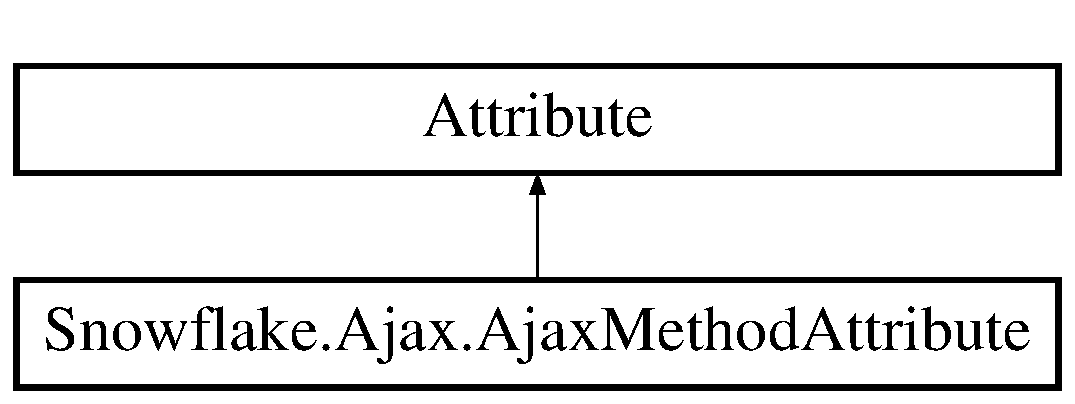
\includegraphics[height=2.000000cm]{class_snowflake_1_1_ajax_1_1_ajax_method_attribute}
\end{center}
\end{figure}
\subsection*{Properties}
\begin{DoxyCompactItemize}
\item 
string \hyperlink{class_snowflake_1_1_ajax_1_1_ajax_method_attribute_ace2bd4864bda17e7a7e6fdb3c4e3d82f}{Method\+Name}\hspace{0.3cm}{\ttfamily  \mbox{[}get, set\mbox{]}}
\begin{DoxyCompactList}\small\item\em The name of the A\+J\+A\+X Method \end{DoxyCompactList}\item 
string \hyperlink{class_snowflake_1_1_ajax_1_1_ajax_method_attribute_a63f45d38381adbe0f3be6d740ccdefab}{Method\+Prefix}\hspace{0.3cm}{\ttfamily  \mbox{[}get, set\mbox{]}}
\begin{DoxyCompactList}\small\item\em The prefix of the A\+J\+A\+X Method This prefix is essentially a sub-\/namespace within the Ajax\+Name\+Space of your \hyperlink{namespace_snowflake_1_1_ajax}{Ajax} plugin 

Game.\+Get\+All\+Games, where \hyperlink{namespace_snowflake_1_1_game}{Game} is the Method\+Prefix\end{DoxyCompactList}\end{DoxyCompactItemize}


\subsection{Detailed Description}
Methods that will be exported in a Ajax\+Namespace plugin should be marked with this attribute Only methods in a \hyperlink{interface_snowflake_1_1_ajax_1_1_i_base_ajax_namespace}{Snowflake.\+Ajax.\+I\+Base\+Ajax\+Namespace} will be callable via \hyperlink{namespace_snowflake_1_1_ajax}{Ajax} 

\begin{DoxySeeAlso}{See also}
\hyperlink{class_snowflake_1_1_ajax_1_1_base_ajax_namespace}{Snowflake.\+Ajax.\+Base\+Ajax\+Namespace}, \hyperlink{interface_snowflake_1_1_ajax_1_1_i_base_ajax_namespace}{Snowflake.\+Ajax.\+I\+Base\+Ajax\+Namespace}


\end{DoxySeeAlso}
for the implementation of  

\subsection{Property Documentation}
\hypertarget{class_snowflake_1_1_ajax_1_1_ajax_method_attribute_ace2bd4864bda17e7a7e6fdb3c4e3d82f}{}\index{Snowflake\+::\+Ajax\+::\+Ajax\+Method\+Attribute@{Snowflake\+::\+Ajax\+::\+Ajax\+Method\+Attribute}!Method\+Name@{Method\+Name}}
\index{Method\+Name@{Method\+Name}!Snowflake\+::\+Ajax\+::\+Ajax\+Method\+Attribute@{Snowflake\+::\+Ajax\+::\+Ajax\+Method\+Attribute}}
\subsubsection[{Method\+Name}]{\setlength{\rightskip}{0pt plus 5cm}string Snowflake.\+Ajax.\+Ajax\+Method\+Attribute.\+Method\+Name\hspace{0.3cm}{\ttfamily [get]}, {\ttfamily [set]}}\label{class_snowflake_1_1_ajax_1_1_ajax_method_attribute_ace2bd4864bda17e7a7e6fdb3c4e3d82f}


The name of the A\+J\+A\+X Method 

\hypertarget{class_snowflake_1_1_ajax_1_1_ajax_method_attribute_a63f45d38381adbe0f3be6d740ccdefab}{}\index{Snowflake\+::\+Ajax\+::\+Ajax\+Method\+Attribute@{Snowflake\+::\+Ajax\+::\+Ajax\+Method\+Attribute}!Method\+Prefix@{Method\+Prefix}}
\index{Method\+Prefix@{Method\+Prefix}!Snowflake\+::\+Ajax\+::\+Ajax\+Method\+Attribute@{Snowflake\+::\+Ajax\+::\+Ajax\+Method\+Attribute}}
\subsubsection[{Method\+Prefix}]{\setlength{\rightskip}{0pt plus 5cm}string Snowflake.\+Ajax.\+Ajax\+Method\+Attribute.\+Method\+Prefix\hspace{0.3cm}{\ttfamily [get]}, {\ttfamily [set]}}\label{class_snowflake_1_1_ajax_1_1_ajax_method_attribute_a63f45d38381adbe0f3be6d740ccdefab}


The prefix of the A\+J\+A\+X Method This prefix is essentially a sub-\/namespace within the Ajax\+Name\+Space of your \hyperlink{namespace_snowflake_1_1_ajax}{Ajax} plugin 

Game.\+Get\+All\+Games, where \hyperlink{namespace_snowflake_1_1_game}{Game} is the Method\+Prefix



The documentation for this class was generated from the following file\+:\begin{DoxyCompactItemize}
\item 
Ajax/Ajax\+Method\+Attribute.\+cs\end{DoxyCompactItemize}

\hypertarget{class_snowflake_1_1_ajax_1_1_base_ajax_namespace}{}\section{Snowflake.\+Ajax.\+Base\+Ajax\+Namespace Class Reference}
\label{class_snowflake_1_1_ajax_1_1_base_ajax_namespace}\index{Snowflake.\+Ajax.\+Base\+Ajax\+Namespace@{Snowflake.\+Ajax.\+Base\+Ajax\+Namespace}}


 


Inheritance diagram for Snowflake.\+Ajax.\+Base\+Ajax\+Namespace\+:\begin{figure}[H]
\begin{center}
\leavevmode
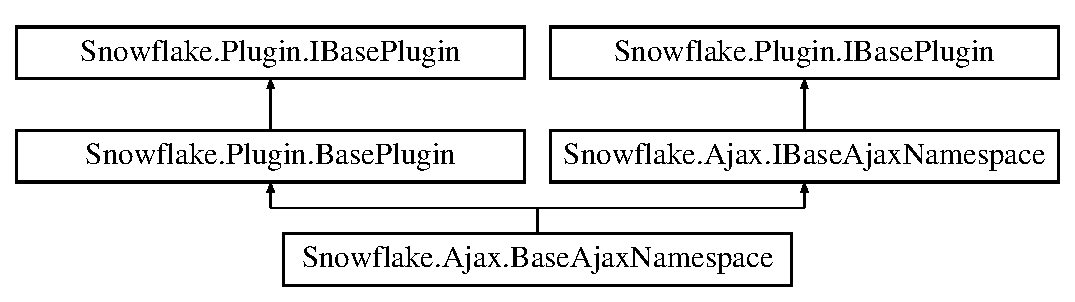
\includegraphics[height=3.000000cm]{class_snowflake_1_1_ajax_1_1_base_ajax_namespace}
\end{center}
\end{figure}
\subsection*{Protected Member Functions}
\begin{DoxyCompactItemize}
\item 
\hypertarget{class_snowflake_1_1_ajax_1_1_base_ajax_namespace_ac0f9fc3b53968a79a37ea929f91a2e12}{}{\bfseries Base\+Ajax\+Namespace} (Assembly plugin\+Assembly, \hyperlink{interface_snowflake_1_1_service_1_1_i_core_service}{I\+Core\+Service} core\+Instance)\label{class_snowflake_1_1_ajax_1_1_base_ajax_namespace_ac0f9fc3b53968a79a37ea929f91a2e12}

\end{DoxyCompactItemize}
\subsection*{Properties}
\begin{DoxyCompactItemize}
\item 
\hypertarget{class_snowflake_1_1_ajax_1_1_base_ajax_namespace_a3dfb53386b78f7433eba3c944cffba85}{}I\+Dictionary$<$ string, Func$<$ \hyperlink{interface_snowflake_1_1_ajax_1_1_i_j_s_request}{I\+J\+S\+Request}, \hyperlink{interface_snowflake_1_1_ajax_1_1_i_j_s_response}{I\+J\+S\+Response} $>$ $>$ {\bfseries Javascript\+Methods}\hspace{0.3cm}{\ttfamily  \mbox{[}get\mbox{]}}\label{class_snowflake_1_1_ajax_1_1_base_ajax_namespace_a3dfb53386b78f7433eba3c944cffba85}

\end{DoxyCompactItemize}
\subsection*{Additional Inherited Members}


\subsection{Detailed Description}


The documentation for this class was generated from the following file\+:\begin{DoxyCompactItemize}
\item 
Ajax/Base\+Ajax\+Namespace.\+cs\end{DoxyCompactItemize}

\hypertarget{class_snowflake_1_1_utility_1_1_base_database}{}\section{Snowflake.\+Utility.\+Base\+Database Class Reference}
\label{class_snowflake_1_1_utility_1_1_base_database}\index{Snowflake.\+Utility.\+Base\+Database@{Snowflake.\+Utility.\+Base\+Database}}
\subsection*{Public Member Functions}
\begin{DoxyCompactItemize}
\item 
\hypertarget{class_snowflake_1_1_utility_1_1_base_database_a9e4af6c69c3ccfdd1b96e5b57647af17}{}{\bfseries Base\+Database} (string file\+Name)\label{class_snowflake_1_1_utility_1_1_base_database_a9e4af6c69c3ccfdd1b96e5b57647af17}

\end{DoxyCompactItemize}
\subsection*{Properties}
\begin{DoxyCompactItemize}
\item 
\hypertarget{class_snowflake_1_1_utility_1_1_base_database_a7f9dd647373f1683b2f43d5ecc64a851}{}string {\bfseries File\+Name}\hspace{0.3cm}{\ttfamily  \mbox{[}get\mbox{]}}\label{class_snowflake_1_1_utility_1_1_base_database_a7f9dd647373f1683b2f43d5ecc64a851}

\item 
\hypertarget{class_snowflake_1_1_utility_1_1_base_database_a05b751ea17d1799614ca78b46166e30a}{}S\+Q\+Lite\+Connection {\bfseries D\+B\+Connection}\hspace{0.3cm}{\ttfamily  \mbox{[}get, set\mbox{]}}\label{class_snowflake_1_1_utility_1_1_base_database_a05b751ea17d1799614ca78b46166e30a}

\end{DoxyCompactItemize}


The documentation for this class was generated from the following file\+:\begin{DoxyCompactItemize}
\item 
Utility/Base\+Database.\+cs\end{DoxyCompactItemize}

\hypertarget{class_snowflake_1_1_service_1_1_http_server_1_1_base_http_server}{}\section{Snowflake.\+Service.\+Http\+Server.\+Base\+Http\+Server Class Reference}
\label{class_snowflake_1_1_service_1_1_http_server_1_1_base_http_server}\index{Snowflake.\+Service.\+Http\+Server.\+Base\+Http\+Server@{Snowflake.\+Service.\+Http\+Server.\+Base\+Http\+Server}}


 


Inheritance diagram for Snowflake.\+Service.\+Http\+Server.\+Base\+Http\+Server\+:\begin{figure}[H]
\begin{center}
\leavevmode
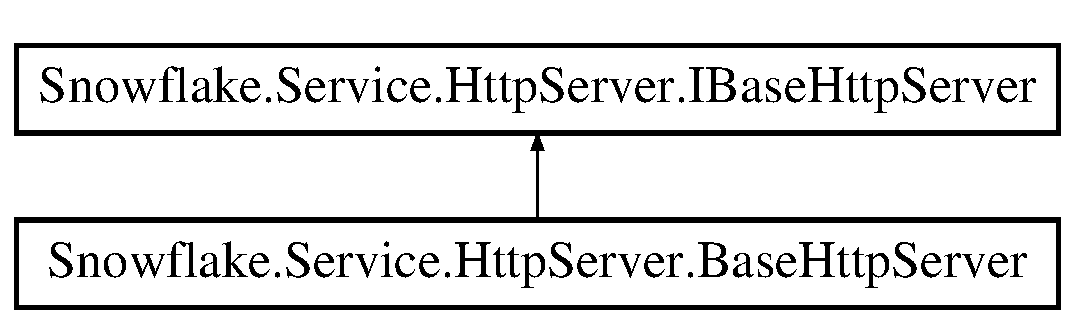
\includegraphics[height=2.000000cm]{class_snowflake_1_1_service_1_1_http_server_1_1_base_http_server}
\end{center}
\end{figure}
\subsection*{Public Member Functions}
\begin{DoxyCompactItemize}
\item 
\hypertarget{class_snowflake_1_1_service_1_1_http_server_1_1_base_http_server_a1d7d941bea5a2d1a8856c0be94a2f1a7}{}{\bfseries Base\+Http\+Server} (int port)\label{class_snowflake_1_1_service_1_1_http_server_1_1_base_http_server_a1d7d941bea5a2d1a8856c0be94a2f1a7}

\item 
\hypertarget{class_snowflake_1_1_service_1_1_http_server_1_1_base_http_server_a277f3db1a4fc105580487c6fa5023df9}{}void {\bfseries Start\+Server} ()\label{class_snowflake_1_1_service_1_1_http_server_1_1_base_http_server_a277f3db1a4fc105580487c6fa5023df9}

\item 
\hypertarget{class_snowflake_1_1_service_1_1_http_server_1_1_base_http_server_a628c25e83a0a971de4009cc325aa78ab}{}void {\bfseries Stop\+Server} ()\label{class_snowflake_1_1_service_1_1_http_server_1_1_base_http_server_a628c25e83a0a971de4009cc325aa78ab}

\end{DoxyCompactItemize}
\subsection*{Protected Member Functions}
\begin{DoxyCompactItemize}
\item 
abstract Task \hyperlink{class_snowflake_1_1_service_1_1_http_server_1_1_base_http_server_a4205e94106204b2738707b88f84c7670}{Process} (Http\+Listener\+Context context)
\begin{DoxyCompactList}\small\item\em Implement this to handle the process loop \end{DoxyCompactList}\end{DoxyCompactItemize}


\subsection{Detailed Description}


\subsection{Member Function Documentation}
\hypertarget{class_snowflake_1_1_service_1_1_http_server_1_1_base_http_server_a4205e94106204b2738707b88f84c7670}{}\index{Snowflake\+::\+Service\+::\+Http\+Server\+::\+Base\+Http\+Server@{Snowflake\+::\+Service\+::\+Http\+Server\+::\+Base\+Http\+Server}!Process@{Process}}
\index{Process@{Process}!Snowflake\+::\+Service\+::\+Http\+Server\+::\+Base\+Http\+Server@{Snowflake\+::\+Service\+::\+Http\+Server\+::\+Base\+Http\+Server}}
\subsubsection[{Process}]{\setlength{\rightskip}{0pt plus 5cm}abstract Task Snowflake.\+Service.\+Http\+Server.\+Base\+Http\+Server.\+Process (
\begin{DoxyParamCaption}
\item[{Http\+Listener\+Context}]{context}
\end{DoxyParamCaption}
)\hspace{0.3cm}{\ttfamily [protected]}, {\ttfamily [pure virtual]}}\label{class_snowflake_1_1_service_1_1_http_server_1_1_base_http_server_a4205e94106204b2738707b88f84c7670}


Implement this to handle the process loop 


\begin{DoxyParams}{Parameters}
{\em context} & The H\+T\+T\+P context of the server listener\\
\hline
\end{DoxyParams}
\begin{DoxyReturn}{Returns}
A Task that is called asynchronously that outputs a stream of text to be written as the Http\+Response
\end{DoxyReturn}
Snowflake.\+Service.\+Server for example implementations 

The documentation for this class was generated from the following file\+:\begin{DoxyCompactItemize}
\item 
Service/\+Http\+Server/Base\+Http\+Server.\+cs\end{DoxyCompactItemize}

\hypertarget{class_snowflake_1_1_plugin_1_1_base_plugin}{}\section{Snowflake.\+Plugin.\+Base\+Plugin Class Reference}
\label{class_snowflake_1_1_plugin_1_1_base_plugin}\index{Snowflake.\+Plugin.\+Base\+Plugin@{Snowflake.\+Plugin.\+Base\+Plugin}}
Inheritance diagram for Snowflake.\+Plugin.\+Base\+Plugin\+:\begin{figure}[H]
\begin{center}
\leavevmode
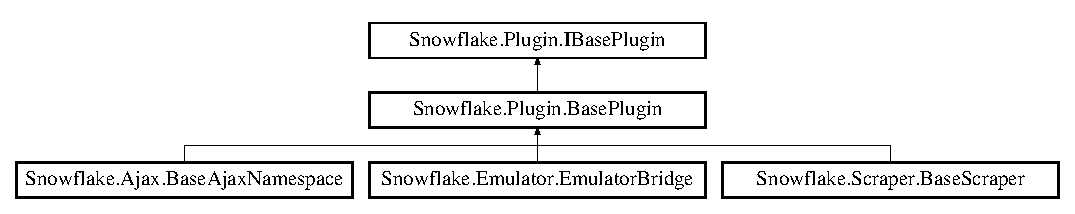
\includegraphics[height=2.434783cm]{class_snowflake_1_1_plugin_1_1_base_plugin}
\end{center}
\end{figure}
\subsection*{Public Member Functions}
\begin{DoxyCompactItemize}
\item 
\hypertarget{class_snowflake_1_1_plugin_1_1_base_plugin_af6ba0fbb132d9dcb8ad26ad4806a353e}{}Stream {\bfseries Get\+Resource} (string resource\+Name)\label{class_snowflake_1_1_plugin_1_1_base_plugin_af6ba0fbb132d9dcb8ad26ad4806a353e}

\end{DoxyCompactItemize}
\subsection*{Protected Member Functions}
\begin{DoxyCompactItemize}
\item 
\hypertarget{class_snowflake_1_1_plugin_1_1_base_plugin_aafe9dc626650dca67a5062a8f794ccab}{}{\bfseries Base\+Plugin} (Assembly plugin\+Assembly, \hyperlink{interface_snowflake_1_1_service_1_1_i_core_service}{I\+Core\+Service} core\+Instance)\label{class_snowflake_1_1_plugin_1_1_base_plugin_aafe9dc626650dca67a5062a8f794ccab}

\end{DoxyCompactItemize}
\subsection*{Properties}
\begin{DoxyCompactItemize}
\item 
\hypertarget{class_snowflake_1_1_plugin_1_1_base_plugin_a4591bc8fb9ea5be53875efaa0349645a}{}string {\bfseries Plugin\+Name}\hspace{0.3cm}{\ttfamily  \mbox{[}get\mbox{]}}\label{class_snowflake_1_1_plugin_1_1_base_plugin_a4591bc8fb9ea5be53875efaa0349645a}

\item 
\hypertarget{class_snowflake_1_1_plugin_1_1_base_plugin_a60c0ea3db85d4a7c4be409b20f7f09f5}{}I\+Dictionary$<$ string, dynamic $>$ {\bfseries Plugin\+Info}\hspace{0.3cm}{\ttfamily  \mbox{[}get\mbox{]}}\label{class_snowflake_1_1_plugin_1_1_base_plugin_a60c0ea3db85d4a7c4be409b20f7f09f5}

\item 
\hypertarget{class_snowflake_1_1_plugin_1_1_base_plugin_ab2809eeec133163a0b8975e702731e14}{}Assembly {\bfseries Plugin\+Assembly}\hspace{0.3cm}{\ttfamily  \mbox{[}get\mbox{]}}\label{class_snowflake_1_1_plugin_1_1_base_plugin_ab2809eeec133163a0b8975e702731e14}

\item 
\hypertarget{class_snowflake_1_1_plugin_1_1_base_plugin_a15ce8469fbc8d41cb898f38a87d6e870}{}string {\bfseries Plugin\+Data\+Path}\hspace{0.3cm}{\ttfamily  \mbox{[}get\mbox{]}}\label{class_snowflake_1_1_plugin_1_1_base_plugin_a15ce8469fbc8d41cb898f38a87d6e870}

\item 
\hypertarget{class_snowflake_1_1_plugin_1_1_base_plugin_a0d4668fd0807bb6914ca20003325a884}{}virtual \hyperlink{interface_snowflake_1_1_plugin_1_1_i_plugin_configuration}{I\+Plugin\+Configuration} {\bfseries Plugin\+Configuration}\hspace{0.3cm}{\ttfamily  \mbox{[}get, protected set\mbox{]}}\label{class_snowflake_1_1_plugin_1_1_base_plugin_a0d4668fd0807bb6914ca20003325a884}

\item 
\hypertarget{class_snowflake_1_1_plugin_1_1_base_plugin_af64e9b0ef81c66e11dac65f0d789a55e}{}\hyperlink{interface_snowflake_1_1_service_1_1_i_core_service}{I\+Core\+Service} {\bfseries Core\+Instance}\hspace{0.3cm}{\ttfamily  \mbox{[}get\mbox{]}}\label{class_snowflake_1_1_plugin_1_1_base_plugin_af64e9b0ef81c66e11dac65f0d789a55e}

\end{DoxyCompactItemize}


The documentation for this class was generated from the following file\+:\begin{DoxyCompactItemize}
\item 
Plugin/Base\+Plugin.\+cs\end{DoxyCompactItemize}

\hypertarget{class_snowflake_1_1_scraper_1_1_base_scraper}{}\section{Snowflake.\+Scraper.\+Base\+Scraper Class Reference}
\label{class_snowflake_1_1_scraper_1_1_base_scraper}\index{Snowflake.\+Scraper.\+Base\+Scraper@{Snowflake.\+Scraper.\+Base\+Scraper}}
Inheritance diagram for Snowflake.\+Scraper.\+Base\+Scraper\+:\begin{figure}[H]
\begin{center}
\leavevmode
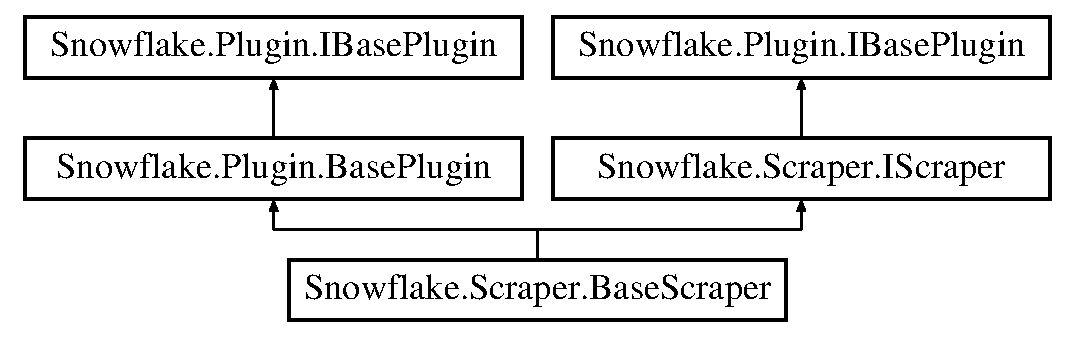
\includegraphics[height=3.000000cm]{class_snowflake_1_1_scraper_1_1_base_scraper}
\end{center}
\end{figure}
\subsection*{Public Member Functions}
\begin{DoxyCompactItemize}
\item 
\hypertarget{class_snowflake_1_1_scraper_1_1_base_scraper_a5f2dbc39aa8b7d461b95eaebd0ba2492}{}abstract I\+List$<$ \hyperlink{interface_snowflake_1_1_scraper_1_1_i_game_scrape_result}{I\+Game\+Scrape\+Result} $>$ {\bfseries Get\+Search\+Results} (string search\+Query)\label{class_snowflake_1_1_scraper_1_1_base_scraper_a5f2dbc39aa8b7d461b95eaebd0ba2492}

\item 
\hypertarget{class_snowflake_1_1_scraper_1_1_base_scraper_a6527a1d267658a527fae3a742f483706}{}abstract I\+List$<$ \hyperlink{interface_snowflake_1_1_scraper_1_1_i_game_scrape_result}{I\+Game\+Scrape\+Result} $>$ {\bfseries Get\+Search\+Results} (string search\+Query, string platform\+Id)\label{class_snowflake_1_1_scraper_1_1_base_scraper_a6527a1d267658a527fae3a742f483706}

\item 
\hypertarget{class_snowflake_1_1_scraper_1_1_base_scraper_a5ba5abf1678db32ff9f4b9c4eaa79e00}{}abstract Tuple$<$ I\+Dictionary$<$ string, string $>$, \hyperlink{interface_snowflake_1_1_scraper_1_1_i_game_images_result}{I\+Game\+Images\+Result} $>$ {\bfseries Get\+Game\+Details} (string id)\label{class_snowflake_1_1_scraper_1_1_base_scraper_a5ba5abf1678db32ff9f4b9c4eaa79e00}

\end{DoxyCompactItemize}
\subsection*{Protected Member Functions}
\begin{DoxyCompactItemize}
\item 
\hypertarget{class_snowflake_1_1_scraper_1_1_base_scraper_aea32ff122e553624603664ff0ca41b56}{}{\bfseries Base\+Scraper} (Assembly plugin\+Assembly, \hyperlink{interface_snowflake_1_1_service_1_1_i_core_service}{I\+Core\+Service} core\+Instance)\label{class_snowflake_1_1_scraper_1_1_base_scraper_aea32ff122e553624603664ff0ca41b56}

\end{DoxyCompactItemize}
\subsection*{Properties}
\begin{DoxyCompactItemize}
\item 
\hypertarget{class_snowflake_1_1_scraper_1_1_base_scraper_ac1f0943f27012e1558e55ee89febf270}{}\hyperlink{class_snowflake_1_1_utility_1_1_bi_dictionary}{Bi\+Dictionary}$<$ string, string $>$ {\bfseries Scraper\+Map}\hspace{0.3cm}{\ttfamily  \mbox{[}get\mbox{]}}\label{class_snowflake_1_1_scraper_1_1_base_scraper_ac1f0943f27012e1558e55ee89febf270}

\end{DoxyCompactItemize}


The documentation for this class was generated from the following file\+:\begin{DoxyCompactItemize}
\item 
Scraper/Base\+Scraper.\+cs\end{DoxyCompactItemize}

\hypertarget{class_snowflake_1_1_utility_1_1_bi_dictionary}{}\section{Snowflake.\+Utility.\+Bi\+Dictionary$<$ T\+First, T\+Second $>$ Class Template Reference}
\label{class_snowflake_1_1_utility_1_1_bi_dictionary}\index{Snowflake.\+Utility.\+Bi\+Dictionary$<$ T\+First, T\+Second $>$@{Snowflake.\+Utility.\+Bi\+Dictionary$<$ T\+First, T\+Second $>$}}
Inheritance diagram for Snowflake.\+Utility.\+Bi\+Dictionary$<$ T\+First, T\+Second $>$\+:\begin{figure}[H]
\begin{center}
\leavevmode
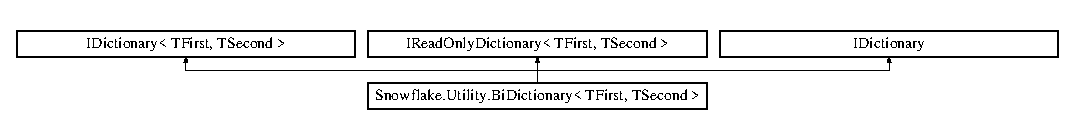
\includegraphics[height=1.244444cm]{class_snowflake_1_1_utility_1_1_bi_dictionary}
\end{center}
\end{figure}
\subsection*{Public Member Functions}
\begin{DoxyCompactItemize}
\item 
\hypertarget{class_snowflake_1_1_utility_1_1_bi_dictionary_ac27cee9bee531be61f24e309875175ea}{}I\+Enumerator$<$ Key\+Value\+Pair$<$ T\+First, T\+Second $>$ $>$ {\bfseries Get\+Enumerator} ()\label{class_snowflake_1_1_utility_1_1_bi_dictionary_ac27cee9bee531be61f24e309875175ea}

\item 
\hypertarget{class_snowflake_1_1_utility_1_1_bi_dictionary_a5355a5a441236c690e09cd3ad9c486ee}{}void {\bfseries Add} (T\+First key, T\+Second value)\label{class_snowflake_1_1_utility_1_1_bi_dictionary_a5355a5a441236c690e09cd3ad9c486ee}

\item 
\hypertarget{class_snowflake_1_1_utility_1_1_bi_dictionary_abc385c341737849597557988e0964459}{}bool {\bfseries Contains\+Key} (T\+First key)\label{class_snowflake_1_1_utility_1_1_bi_dictionary_abc385c341737849597557988e0964459}

\item 
\hypertarget{class_snowflake_1_1_utility_1_1_bi_dictionary_a43f67acac646a57bcf8f3b4d73b0c96d}{}bool {\bfseries Try\+Get\+Value} (T\+First key, out T\+Second value)\label{class_snowflake_1_1_utility_1_1_bi_dictionary_a43f67acac646a57bcf8f3b4d73b0c96d}

\item 
\hypertarget{class_snowflake_1_1_utility_1_1_bi_dictionary_a0189b2ea0bc2e9ec6d63bb8467e2b345}{}bool {\bfseries Remove} (T\+First key)\label{class_snowflake_1_1_utility_1_1_bi_dictionary_a0189b2ea0bc2e9ec6d63bb8467e2b345}

\item 
\hypertarget{class_snowflake_1_1_utility_1_1_bi_dictionary_a856eda45fe6978a3396260f296bd8c3d}{}void {\bfseries Clear} ()\label{class_snowflake_1_1_utility_1_1_bi_dictionary_a856eda45fe6978a3396260f296bd8c3d}

\end{DoxyCompactItemize}
\subsection*{Properties}
\begin{DoxyCompactItemize}
\item 
\hypertarget{class_snowflake_1_1_utility_1_1_bi_dictionary_aca11c62f168fcf073fea26d9282a4766}{}I\+Dictionary$<$ T\+Second, T\+First $>$ {\bfseries Reverse}\hspace{0.3cm}{\ttfamily  \mbox{[}get\mbox{]}}\label{class_snowflake_1_1_utility_1_1_bi_dictionary_aca11c62f168fcf073fea26d9282a4766}

\item 
\hypertarget{class_snowflake_1_1_utility_1_1_bi_dictionary_ae9acd45d5a8ad6bae0863db2bfee735e}{}int {\bfseries Count}\hspace{0.3cm}{\ttfamily  \mbox{[}get\mbox{]}}\label{class_snowflake_1_1_utility_1_1_bi_dictionary_ae9acd45d5a8ad6bae0863db2bfee735e}

\item 
\hypertarget{class_snowflake_1_1_utility_1_1_bi_dictionary_a017281d17e3045e64315de4418ddc786}{}bool {\bfseries Is\+Read\+Only}\hspace{0.3cm}{\ttfamily  \mbox{[}get\mbox{]}}\label{class_snowflake_1_1_utility_1_1_bi_dictionary_a017281d17e3045e64315de4418ddc786}

\item 
\hypertarget{class_snowflake_1_1_utility_1_1_bi_dictionary_a8ea22f205d3a1fba93a5e78a84cc808c}{}T\+Second {\bfseries this\mbox{[}\+T\+First key\mbox{]}}\hspace{0.3cm}{\ttfamily  \mbox{[}get, set\mbox{]}}\label{class_snowflake_1_1_utility_1_1_bi_dictionary_a8ea22f205d3a1fba93a5e78a84cc808c}

\item 
\hypertarget{class_snowflake_1_1_utility_1_1_bi_dictionary_a3fff4ccfda66b4b6db5547959d20a2dc}{}I\+Collection$<$ T\+First $>$ {\bfseries Keys}\hspace{0.3cm}{\ttfamily  \mbox{[}get\mbox{]}}\label{class_snowflake_1_1_utility_1_1_bi_dictionary_a3fff4ccfda66b4b6db5547959d20a2dc}

\item 
\hypertarget{class_snowflake_1_1_utility_1_1_bi_dictionary_aaf36989a9f6f3b43142c96a8b00afcef}{}I\+Collection$<$ T\+Second $>$ {\bfseries Values}\hspace{0.3cm}{\ttfamily  \mbox{[}get\mbox{]}}\label{class_snowflake_1_1_utility_1_1_bi_dictionary_aaf36989a9f6f3b43142c96a8b00afcef}

\end{DoxyCompactItemize}


The documentation for this class was generated from the following file\+:\begin{DoxyCompactItemize}
\item 
Utility/Bi\+Dictionary.\+cs\end{DoxyCompactItemize}

\hypertarget{class_snowflake_1_1_utility_1_1_crc32}{}\section{Snowflake.\+Utility.\+Crc32 Class Reference}
\label{class_snowflake_1_1_utility_1_1_crc32}\index{Snowflake.\+Utility.\+Crc32@{Snowflake.\+Utility.\+Crc32}}


Implements a 32-\/bit C\+R\+C hash algorithm compatible with Zip etc.  


Inheritance diagram for Snowflake.\+Utility.\+Crc32\+:\begin{figure}[H]
\begin{center}
\leavevmode
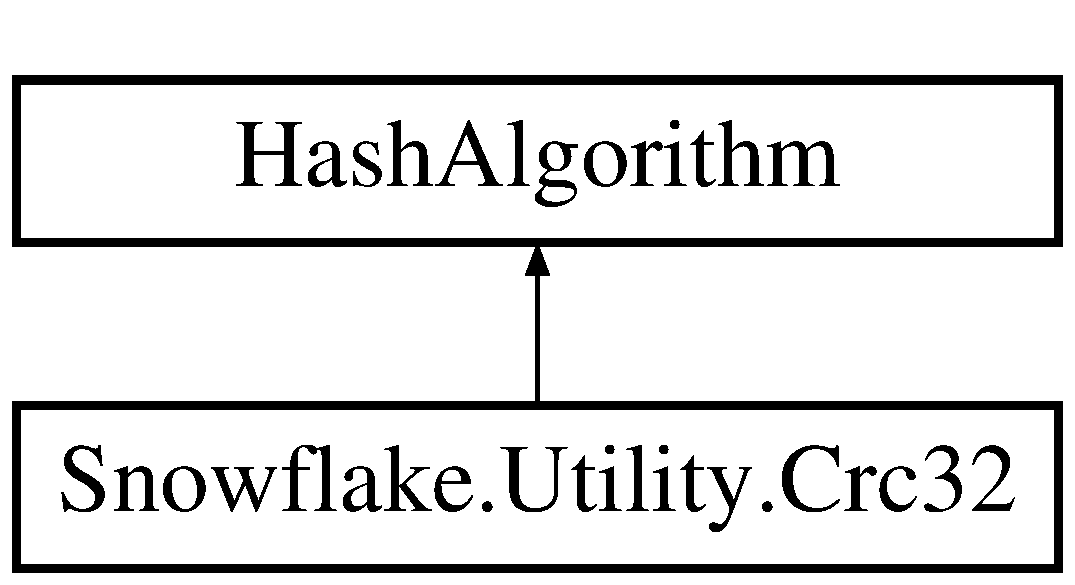
\includegraphics[height=2.000000cm]{class_snowflake_1_1_utility_1_1_crc32}
\end{center}
\end{figure}
\subsection*{Public Member Functions}
\begin{DoxyCompactItemize}
\item 
\hypertarget{class_snowflake_1_1_utility_1_1_crc32_a90e52671edd3e953485905054c094ae3}{}{\bfseries Crc32} (U\+Int32 polynomial, U\+Int32 seed)\label{class_snowflake_1_1_utility_1_1_crc32_a90e52671edd3e953485905054c094ae3}

\item 
\hypertarget{class_snowflake_1_1_utility_1_1_crc32_ad148a1dd67a36490f8ff24f3aa753341}{}override void {\bfseries Initialize} ()\label{class_snowflake_1_1_utility_1_1_crc32_ad148a1dd67a36490f8ff24f3aa753341}

\end{DoxyCompactItemize}
\subsection*{Static Public Member Functions}
\begin{DoxyCompactItemize}
\item 
\hypertarget{class_snowflake_1_1_utility_1_1_crc32_a7a213babf0c0906d5d2f7b2325f1b93d}{}static U\+Int32 {\bfseries Compute} (byte\mbox{[}$\,$\mbox{]} buffer)\label{class_snowflake_1_1_utility_1_1_crc32_a7a213babf0c0906d5d2f7b2325f1b93d}

\item 
\hypertarget{class_snowflake_1_1_utility_1_1_crc32_a7064144245a3b084fd02b4bbb86e947d}{}static U\+Int32 {\bfseries Compute} (U\+Int32 seed, byte\mbox{[}$\,$\mbox{]} buffer)\label{class_snowflake_1_1_utility_1_1_crc32_a7064144245a3b084fd02b4bbb86e947d}

\item 
\hypertarget{class_snowflake_1_1_utility_1_1_crc32_a0f86bf9e182c258db61b4ae51bf1479c}{}static U\+Int32 {\bfseries Compute} (U\+Int32 polynomial, U\+Int32 seed, byte\mbox{[}$\,$\mbox{]} buffer)\label{class_snowflake_1_1_utility_1_1_crc32_a0f86bf9e182c258db61b4ae51bf1479c}

\item 
\hypertarget{class_snowflake_1_1_utility_1_1_crc32_ad56dbb47725d2d8e85fb42c0fc535b67}{}static string {\bfseries Get\+Crc32} (File\+Stream file)\label{class_snowflake_1_1_utility_1_1_crc32_ad56dbb47725d2d8e85fb42c0fc535b67}

\item 
\hypertarget{class_snowflake_1_1_utility_1_1_crc32_ae38f0258308028c6ac121f9c3fdf9544}{}static string {\bfseries Get\+Crc32} (string file\+Name)\label{class_snowflake_1_1_utility_1_1_crc32_ae38f0258308028c6ac121f9c3fdf9544}

\end{DoxyCompactItemize}
\subsection*{Public Attributes}
\begin{DoxyCompactItemize}
\item 
\hypertarget{class_snowflake_1_1_utility_1_1_crc32_a0c1ef2a44440c814edb8d5db345b4fb8}{}const U\+Int32 {\bfseries Default\+Polynomial} = 0xedb88320u\label{class_snowflake_1_1_utility_1_1_crc32_a0c1ef2a44440c814edb8d5db345b4fb8}

\item 
\hypertarget{class_snowflake_1_1_utility_1_1_crc32_aaa9368fd3ae31f87beb2e975ed66e6c7}{}const U\+Int32 {\bfseries Default\+Seed} = 0xffffffffu\label{class_snowflake_1_1_utility_1_1_crc32_aaa9368fd3ae31f87beb2e975ed66e6c7}

\end{DoxyCompactItemize}
\subsection*{Protected Member Functions}
\begin{DoxyCompactItemize}
\item 
\hypertarget{class_snowflake_1_1_utility_1_1_crc32_a9635cc0df05fa4e079dfefffd801d645}{}override void {\bfseries Hash\+Core} (byte\mbox{[}$\,$\mbox{]} buffer, int start, int length)\label{class_snowflake_1_1_utility_1_1_crc32_a9635cc0df05fa4e079dfefffd801d645}

\item 
\hypertarget{class_snowflake_1_1_utility_1_1_crc32_a25a0409f3cffe53b07eff8a4571c43e4}{}override byte\mbox{[}$\,$\mbox{]} {\bfseries Hash\+Final} ()\label{class_snowflake_1_1_utility_1_1_crc32_a25a0409f3cffe53b07eff8a4571c43e4}

\end{DoxyCompactItemize}
\subsection*{Properties}
\begin{DoxyCompactItemize}
\item 
\hypertarget{class_snowflake_1_1_utility_1_1_crc32_a51ac41a193610f9cdbdeec294b61e804}{}override int {\bfseries Hash\+Size}\hspace{0.3cm}{\ttfamily  \mbox{[}get\mbox{]}}\label{class_snowflake_1_1_utility_1_1_crc32_a51ac41a193610f9cdbdeec294b61e804}

\end{DoxyCompactItemize}


\subsection{Detailed Description}
Implements a 32-\/bit C\+R\+C hash algorithm compatible with Zip etc. 

\hyperlink{class_snowflake_1_1_utility_1_1_crc32}{Crc32} should only be used for backward compatibility with older file formats and algorithms. It is not secure enough for new applications. If you need to call multiple times for the same data either use the Hash\+Algorithm interface or remember that the result of one Compute call needs to be $\sim$ (X\+O\+R) before being passed in as the seed for the next Compute call. 

The documentation for this class was generated from the following file\+:\begin{DoxyCompactItemize}
\item 
Utility/Crc32.\+cs\end{DoxyCompactItemize}

\hypertarget{class_snowflake_1_1_emulator_1_1_emulator_bridge}{}\section{Snowflake.\+Emulator.\+Emulator\+Bridge Class Reference}
\label{class_snowflake_1_1_emulator_1_1_emulator_bridge}\index{Snowflake.\+Emulator.\+Emulator\+Bridge@{Snowflake.\+Emulator.\+Emulator\+Bridge}}
Inheritance diagram for Snowflake.\+Emulator.\+Emulator\+Bridge\+:\begin{figure}[H]
\begin{center}
\leavevmode
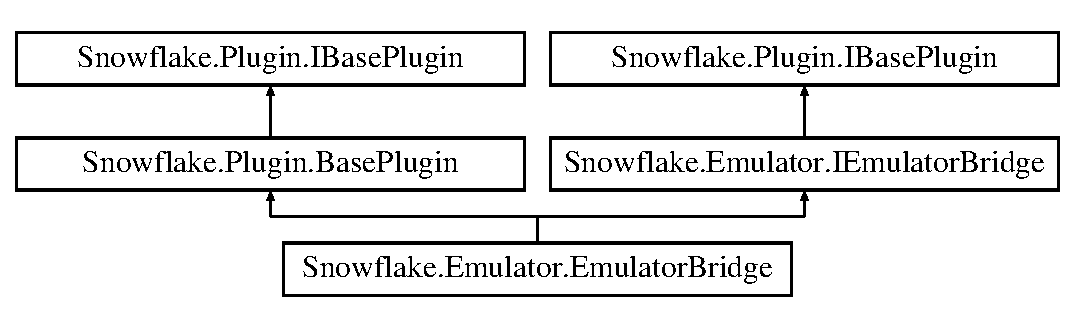
\includegraphics[height=3.000000cm]{class_snowflake_1_1_emulator_1_1_emulator_bridge}
\end{center}
\end{figure}
\subsection*{Public Member Functions}
\begin{DoxyCompactItemize}
\item 
\hypertarget{class_snowflake_1_1_emulator_1_1_emulator_bridge_a46acb4aff8c003cc5b0d42b30dc8cd51}{}{\bfseries Emulator\+Bridge} (Assembly plugin\+Assembly, \hyperlink{interface_snowflake_1_1_service_1_1_i_core_service}{I\+Core\+Service} core\+Instance)\label{class_snowflake_1_1_emulator_1_1_emulator_bridge_a46acb4aff8c003cc5b0d42b30dc8cd51}

\item 
\hypertarget{class_snowflake_1_1_emulator_1_1_emulator_bridge_ab490b050c553a114bad5a060dfed8e2f}{}abstract void {\bfseries Start\+Rom} (\hyperlink{interface_snowflake_1_1_game_1_1_i_game_info}{I\+Game\+Info} game\+Info)\label{class_snowflake_1_1_emulator_1_1_emulator_bridge_ab490b050c553a114bad5a060dfed8e2f}

\item 
\hypertarget{class_snowflake_1_1_emulator_1_1_emulator_bridge_acd1ee415922abfd0313929009858b2b4}{}abstract void {\bfseries Handle\+Prompt} (string messagge)\label{class_snowflake_1_1_emulator_1_1_emulator_bridge_acd1ee415922abfd0313929009858b2b4}

\item 
\hypertarget{class_snowflake_1_1_emulator_1_1_emulator_bridge_a19b6a6f5152034a83365a8a9ea8a03ce}{}abstract void {\bfseries Shutdown\+Emulator} ()\label{class_snowflake_1_1_emulator_1_1_emulator_bridge_a19b6a6f5152034a83365a8a9ea8a03ce}

\item 
\hypertarget{class_snowflake_1_1_emulator_1_1_emulator_bridge_a375d797ed11753acd00ae51a45deeaa8}{}virtual string {\bfseries Compile\+Configuration} (\hyperlink{interface_snowflake_1_1_emulator_1_1_configuration_1_1_i_configuration_profile}{I\+Configuration\+Profile} config\+Profile)\label{class_snowflake_1_1_emulator_1_1_emulator_bridge_a375d797ed11753acd00ae51a45deeaa8}

\item 
\hypertarget{class_snowflake_1_1_emulator_1_1_emulator_bridge_ab91a1f58daf7c7474155278db611ad2d}{}virtual string {\bfseries Compile\+Configuration} (\hyperlink{interface_snowflake_1_1_emulator_1_1_configuration_1_1_i_configuration_template}{I\+Configuration\+Template} config\+Template, \hyperlink{interface_snowflake_1_1_emulator_1_1_configuration_1_1_i_configuration_profile}{I\+Configuration\+Profile} config\+Profile)\label{class_snowflake_1_1_emulator_1_1_emulator_bridge_ab91a1f58daf7c7474155278db611ad2d}

\item 
\hypertarget{class_snowflake_1_1_emulator_1_1_emulator_bridge_a1bf84f1df6c8610573929940c320a313}{}virtual string {\bfseries Compile\+Controller} (int player\+Index, \hyperlink{interface_snowflake_1_1_platform_1_1_i_platform_info}{I\+Platform\+Info} platform\+Info, \hyperlink{interface_snowflake_1_1_emulator_1_1_input_1_1_i_input_template}{I\+Input\+Template} input\+Template)\label{class_snowflake_1_1_emulator_1_1_emulator_bridge_a1bf84f1df6c8610573929940c320a313}

\item 
\hypertarget{class_snowflake_1_1_emulator_1_1_emulator_bridge_aa1b0372b02ee8149d9557fe8ed0865fa}{}virtual string {\bfseries Compile\+Controller} (int player\+Index, \hyperlink{interface_snowflake_1_1_controller_1_1_i_controller_definition}{I\+Controller\+Definition} controller\+Definition, \hyperlink{interface_snowflake_1_1_emulator_1_1_input_1_1_i_controller_template}{I\+Controller\+Template} controller\+Template, \hyperlink{interface_snowflake_1_1_controller_1_1_i_controller_profile}{I\+Controller\+Profile} controller\+Profile, \hyperlink{interface_snowflake_1_1_emulator_1_1_input_1_1_i_input_template}{I\+Input\+Template} input\+Template)\label{class_snowflake_1_1_emulator_1_1_emulator_bridge_aa1b0372b02ee8149d9557fe8ed0865fa}

\end{DoxyCompactItemize}
\subsection*{Properties}
\begin{DoxyCompactItemize}
\item 
\hypertarget{class_snowflake_1_1_emulator_1_1_emulator_bridge_a36a0729805c8a6f4310be623a8aac378}{}I\+Dictionary$<$ string, \hyperlink{interface_snowflake_1_1_emulator_1_1_input_1_1_i_controller_template}{I\+Controller\+Template} $>$ {\bfseries Controller\+Templates}\hspace{0.3cm}{\ttfamily  \mbox{[}get\mbox{]}}\label{class_snowflake_1_1_emulator_1_1_emulator_bridge_a36a0729805c8a6f4310be623a8aac378}

\item 
\hypertarget{class_snowflake_1_1_emulator_1_1_emulator_bridge_ad9edcddfd91354fa25ce8d533bbec4fe}{}I\+Dictionary$<$ string, \hyperlink{interface_snowflake_1_1_emulator_1_1_input_1_1_i_input_template}{I\+Input\+Template} $>$ {\bfseries Input\+Templates}\hspace{0.3cm}{\ttfamily  \mbox{[}get\mbox{]}}\label{class_snowflake_1_1_emulator_1_1_emulator_bridge_ad9edcddfd91354fa25ce8d533bbec4fe}

\item 
\hypertarget{class_snowflake_1_1_emulator_1_1_emulator_bridge_a0831dcad2a39ac6b776a93bc9a90170f}{}I\+Dictionary$<$ string, \hyperlink{interface_snowflake_1_1_emulator_1_1_configuration_1_1_i_configuration_template}{I\+Configuration\+Template} $>$ {\bfseries Configuration\+Templates}\hspace{0.3cm}{\ttfamily  \mbox{[}get\mbox{]}}\label{class_snowflake_1_1_emulator_1_1_emulator_bridge_a0831dcad2a39ac6b776a93bc9a90170f}

\item 
\hypertarget{class_snowflake_1_1_emulator_1_1_emulator_bridge_aeb94bd38fdc783239fe507d9ab644d3f}{}I\+List$<$ string $>$ {\bfseries Supported\+Platforms}\hspace{0.3cm}{\ttfamily  \mbox{[}get\mbox{]}}\label{class_snowflake_1_1_emulator_1_1_emulator_bridge_aeb94bd38fdc783239fe507d9ab644d3f}

\item 
\hypertarget{class_snowflake_1_1_emulator_1_1_emulator_bridge_a0390fcb8d486e087e8ef41b59d3bd491}{}\hyperlink{interface_snowflake_1_1_emulator_1_1_i_emulator_assembly}{I\+Emulator\+Assembly} {\bfseries Emulator\+Assembly}\hspace{0.3cm}{\ttfamily  \mbox{[}get\mbox{]}}\label{class_snowflake_1_1_emulator_1_1_emulator_bridge_a0390fcb8d486e087e8ef41b59d3bd491}

\end{DoxyCompactItemize}
\subsection*{Additional Inherited Members}


The documentation for this class was generated from the following file\+:\begin{DoxyCompactItemize}
\item 
Emulator/Emulator\+Bridge.\+cs\end{DoxyCompactItemize}

\hypertarget{interface_snowflake_1_1_service_1_1_manager_1_1_i_ajax_manager}{}\section{Snowflake.\+Service.\+Manager.\+I\+Ajax\+Manager Interface Reference}
\label{interface_snowflake_1_1_service_1_1_manager_1_1_i_ajax_manager}\index{Snowflake.\+Service.\+Manager.\+I\+Ajax\+Manager@{Snowflake.\+Service.\+Manager.\+I\+Ajax\+Manager}}
Inheritance diagram for Snowflake.\+Service.\+Manager.\+I\+Ajax\+Manager\+:\begin{figure}[H]
\begin{center}
\leavevmode
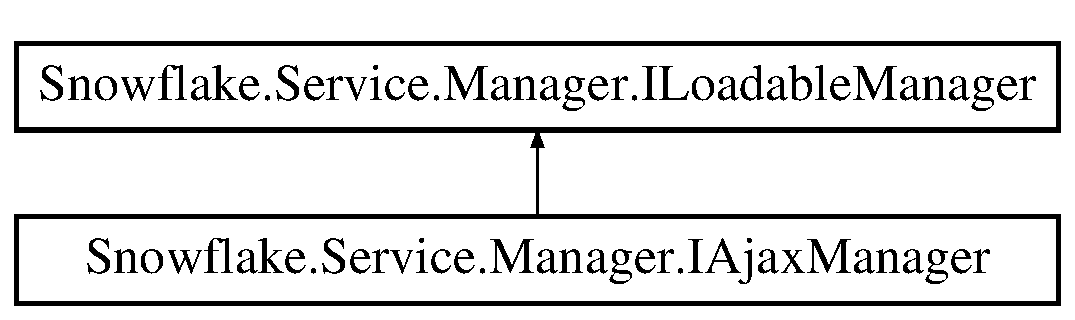
\includegraphics[height=2.000000cm]{interface_snowflake_1_1_service_1_1_manager_1_1_i_ajax_manager}
\end{center}
\end{figure}
\subsection*{Public Member Functions}
\begin{DoxyCompactItemize}
\item 
\hypertarget{interface_snowflake_1_1_service_1_1_manager_1_1_i_ajax_manager_a3ad54521d13be90a1780aed2bf405c92}{}void {\bfseries Register\+Namespace} (string namespace\+Name, \hyperlink{interface_snowflake_1_1_ajax_1_1_i_base_ajax_namespace}{I\+Base\+Ajax\+Namespace} namespace\+Object)\label{interface_snowflake_1_1_service_1_1_manager_1_1_i_ajax_manager_a3ad54521d13be90a1780aed2bf405c92}

\item 
\hypertarget{interface_snowflake_1_1_service_1_1_manager_1_1_i_ajax_manager_a3c8f17ccbe4db1b0912d924107e098ef}{}Task$<$ string $>$ {\bfseries Call\+Method\+Async} (\hyperlink{interface_snowflake_1_1_ajax_1_1_i_j_s_request}{I\+J\+S\+Request} request)\label{interface_snowflake_1_1_service_1_1_manager_1_1_i_ajax_manager_a3c8f17ccbe4db1b0912d924107e098ef}

\item 
\hypertarget{interface_snowflake_1_1_service_1_1_manager_1_1_i_ajax_manager_a5bdf8f37a2d4b40f1e9eaf68ccfa4e31}{}string {\bfseries Call\+Method} (\hyperlink{interface_snowflake_1_1_ajax_1_1_i_j_s_request}{I\+J\+S\+Request} request)\label{interface_snowflake_1_1_service_1_1_manager_1_1_i_ajax_manager_a5bdf8f37a2d4b40f1e9eaf68ccfa4e31}

\end{DoxyCompactItemize}
\subsection*{Properties}
\begin{DoxyCompactItemize}
\item 
\hypertarget{interface_snowflake_1_1_service_1_1_manager_1_1_i_ajax_manager_ab615c30c63704deb66fcc9b22fe95a64}{}I\+Read\+Only\+Dictionary$<$ string, \hyperlink{interface_snowflake_1_1_ajax_1_1_i_base_ajax_namespace}{I\+Base\+Ajax\+Namespace} $>$ {\bfseries Global\+Namespace}\hspace{0.3cm}{\ttfamily  \mbox{[}get\mbox{]}}\label{interface_snowflake_1_1_service_1_1_manager_1_1_i_ajax_manager_ab615c30c63704deb66fcc9b22fe95a64}

\end{DoxyCompactItemize}


The documentation for this interface was generated from the following file\+:\begin{DoxyCompactItemize}
\item 
Service/\+Manager/I\+Ajax\+Manager.\+cs\end{DoxyCompactItemize}

\hypertarget{interface_snowflake_1_1_ajax_1_1_i_base_ajax_namespace}{}\section{Snowflake.\+Ajax.\+I\+Base\+Ajax\+Namespace Interface Reference}
\label{interface_snowflake_1_1_ajax_1_1_i_base_ajax_namespace}\index{Snowflake.\+Ajax.\+I\+Base\+Ajax\+Namespace@{Snowflake.\+Ajax.\+I\+Base\+Ajax\+Namespace}}


Methods to be callable via the Ajax\+Manager should be contained in an \hyperlink{interface_snowflake_1_1_ajax_1_1_i_base_ajax_namespace}{I\+Base\+Ajax\+Namespace} plugin. Snowflake.\+Ajax.\+Base\+Plugin for the implementation  


Inheritance diagram for Snowflake.\+Ajax.\+I\+Base\+Ajax\+Namespace\+:\begin{figure}[H]
\begin{center}
\leavevmode
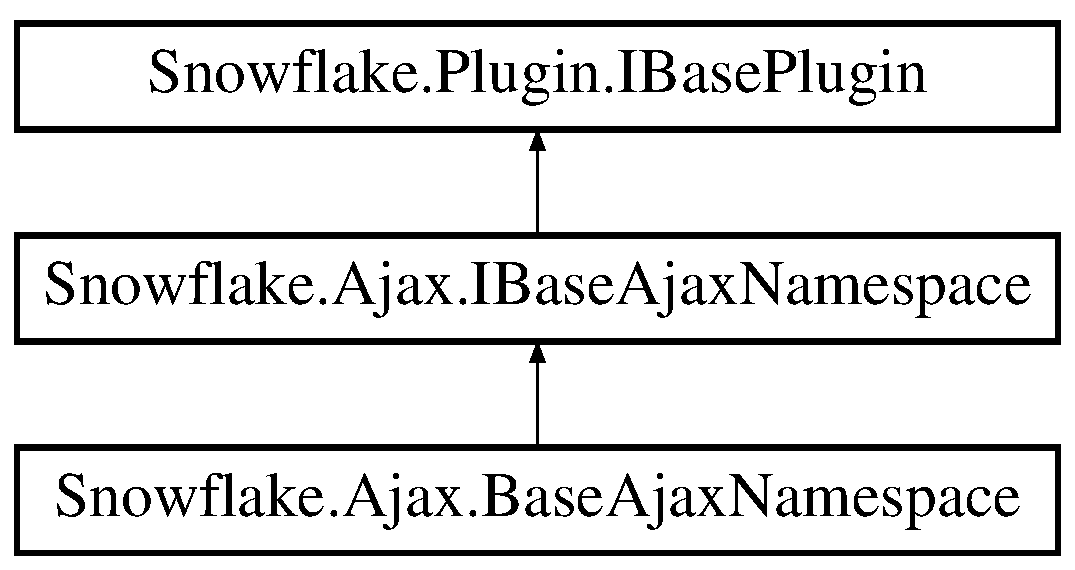
\includegraphics[height=3.000000cm]{interface_snowflake_1_1_ajax_1_1_i_base_ajax_namespace}
\end{center}
\end{figure}
\subsection*{Properties}
\begin{DoxyCompactItemize}
\item 
I\+Dictionary$<$ string, Func$<$ \hyperlink{interface_snowflake_1_1_ajax_1_1_i_j_s_request}{I\+J\+S\+Request}, \hyperlink{interface_snowflake_1_1_ajax_1_1_i_j_s_response}{I\+J\+S\+Response} $>$ $>$ \hyperlink{interface_snowflake_1_1_ajax_1_1_i_base_ajax_namespace_a2b4acf2a85e2c08b0037604021670df0}{Javascript\+Methods}\hspace{0.3cm}{\ttfamily  \mbox{[}get\mbox{]}}
\begin{DoxyCompactList}\small\item\em The generated dictionary of Javascript Methods \end{DoxyCompactList}\end{DoxyCompactItemize}
\subsection*{Additional Inherited Members}


\subsection{Detailed Description}
Methods to be callable via the Ajax\+Manager should be contained in an \hyperlink{interface_snowflake_1_1_ajax_1_1_i_base_ajax_namespace}{I\+Base\+Ajax\+Namespace} plugin. Snowflake.\+Ajax.\+Base\+Plugin for the implementation 



\subsection{Property Documentation}
\hypertarget{interface_snowflake_1_1_ajax_1_1_i_base_ajax_namespace_a2b4acf2a85e2c08b0037604021670df0}{}\index{Snowflake\+::\+Ajax\+::\+I\+Base\+Ajax\+Namespace@{Snowflake\+::\+Ajax\+::\+I\+Base\+Ajax\+Namespace}!Javascript\+Methods@{Javascript\+Methods}}
\index{Javascript\+Methods@{Javascript\+Methods}!Snowflake\+::\+Ajax\+::\+I\+Base\+Ajax\+Namespace@{Snowflake\+::\+Ajax\+::\+I\+Base\+Ajax\+Namespace}}
\subsubsection[{Javascript\+Methods}]{\setlength{\rightskip}{0pt plus 5cm}I\+Dictionary$<$string, Func$<${\bf I\+J\+S\+Request}, {\bf I\+J\+S\+Response}$>$ $>$ Snowflake.\+Ajax.\+I\+Base\+Ajax\+Namespace.\+Javascript\+Methods\hspace{0.3cm}{\ttfamily [get]}}\label{interface_snowflake_1_1_ajax_1_1_i_base_ajax_namespace_a2b4acf2a85e2c08b0037604021670df0}


The generated dictionary of Javascript Methods 



The documentation for this interface was generated from the following file\+:\begin{DoxyCompactItemize}
\item 
Ajax/I\+Base\+Ajax\+Namespace.\+cs\end{DoxyCompactItemize}

\hypertarget{interface_snowflake_1_1_service_1_1_http_server_1_1_i_base_http_server}{}\section{Snowflake.\+Service.\+Http\+Server.\+I\+Base\+Http\+Server Interface Reference}
\label{interface_snowflake_1_1_service_1_1_http_server_1_1_i_base_http_server}\index{Snowflake.\+Service.\+Http\+Server.\+I\+Base\+Http\+Server@{Snowflake.\+Service.\+Http\+Server.\+I\+Base\+Http\+Server}}


Represents an \hyperlink{namespace_snowflake_1_1_service_1_1_http_server}{Http\+Server} that can be used to serve content. Snowflake.\+Server.\+Http\+Server.\+Process(\+Mono.\+Net.\+Http\+Listener\+Context) on how to implement the server loop  


Inheritance diagram for Snowflake.\+Service.\+Http\+Server.\+I\+Base\+Http\+Server\+:\begin{figure}[H]
\begin{center}
\leavevmode
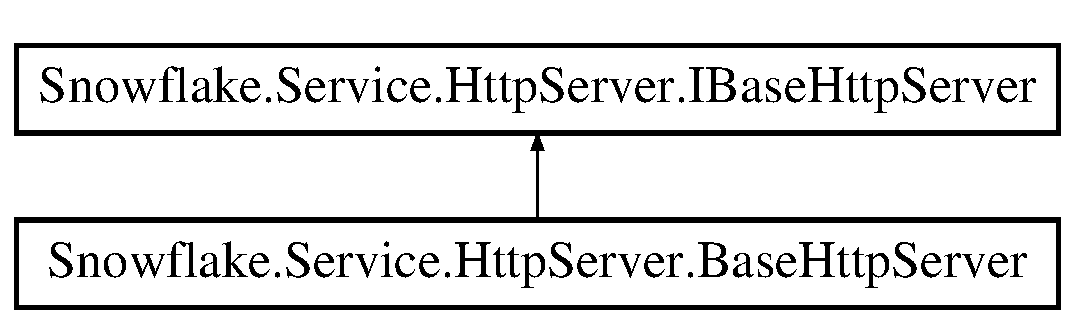
\includegraphics[height=2.000000cm]{interface_snowflake_1_1_service_1_1_http_server_1_1_i_base_http_server}
\end{center}
\end{figure}
\subsection*{Public Member Functions}
\begin{DoxyCompactItemize}
\item 
\hypertarget{interface_snowflake_1_1_service_1_1_http_server_1_1_i_base_http_server_a6c5176f890ae4f1b0e8e7301e11f173d}{}void {\bfseries Start\+Server} ()\label{interface_snowflake_1_1_service_1_1_http_server_1_1_i_base_http_server_a6c5176f890ae4f1b0e8e7301e11f173d}

\item 
\hypertarget{interface_snowflake_1_1_service_1_1_http_server_1_1_i_base_http_server_ae05a22e1d5ae8cacf6d825c080e56020}{}void {\bfseries Stop\+Server} ()\label{interface_snowflake_1_1_service_1_1_http_server_1_1_i_base_http_server_ae05a22e1d5ae8cacf6d825c080e56020}

\end{DoxyCompactItemize}


\subsection{Detailed Description}
Represents an \hyperlink{namespace_snowflake_1_1_service_1_1_http_server}{Http\+Server} that can be used to serve content. Snowflake.\+Server.\+Http\+Server.\+Process(\+Mono.\+Net.\+Http\+Listener\+Context) on how to implement the server loop 



The documentation for this interface was generated from the following file\+:\begin{DoxyCompactItemize}
\item 
Service/\+Http\+Server/I\+Base\+Http\+Server.\+cs\end{DoxyCompactItemize}

\hypertarget{interface_snowflake_1_1_plugin_1_1_i_base_plugin}{}\section{Snowflake.\+Plugin.\+I\+Base\+Plugin Interface Reference}
\label{interface_snowflake_1_1_plugin_1_1_i_base_plugin}\index{Snowflake.\+Plugin.\+I\+Base\+Plugin@{Snowflake.\+Plugin.\+I\+Base\+Plugin}}
Inheritance diagram for Snowflake.\+Plugin.\+I\+Base\+Plugin\+:\begin{figure}[H]
\begin{center}
\leavevmode
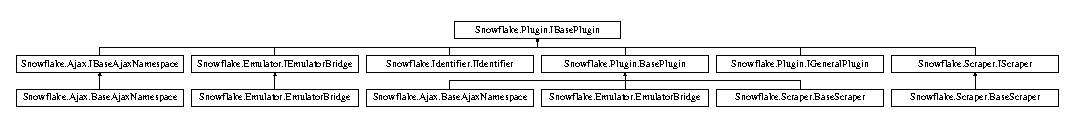
\includegraphics[height=1.201717cm]{interface_snowflake_1_1_plugin_1_1_i_base_plugin}
\end{center}
\end{figure}
\subsection*{Public Member Functions}
\begin{DoxyCompactItemize}
\item 
\hypertarget{interface_snowflake_1_1_plugin_1_1_i_base_plugin_aa1feaad7a3b4ce6fd82bfd180e99a876}{}Stream {\bfseries Get\+Resource} (string resource\+Name)\label{interface_snowflake_1_1_plugin_1_1_i_base_plugin_aa1feaad7a3b4ce6fd82bfd180e99a876}

\end{DoxyCompactItemize}
\subsection*{Properties}
\begin{DoxyCompactItemize}
\item 
\hypertarget{interface_snowflake_1_1_plugin_1_1_i_base_plugin_a3d9484a7b0baeb1ad2b96166abc6e86c}{}string {\bfseries Plugin\+Name}\hspace{0.3cm}{\ttfamily  \mbox{[}get\mbox{]}}\label{interface_snowflake_1_1_plugin_1_1_i_base_plugin_a3d9484a7b0baeb1ad2b96166abc6e86c}

\item 
\hypertarget{interface_snowflake_1_1_plugin_1_1_i_base_plugin_acffa36d28a9af2e65b9d78ee57990627}{}string {\bfseries Plugin\+Data\+Path}\hspace{0.3cm}{\ttfamily  \mbox{[}get\mbox{]}}\label{interface_snowflake_1_1_plugin_1_1_i_base_plugin_acffa36d28a9af2e65b9d78ee57990627}

\item 
\hypertarget{interface_snowflake_1_1_plugin_1_1_i_base_plugin_a90fe77196a24fd7dd23b5152daa51828}{}Assembly {\bfseries Plugin\+Assembly}\hspace{0.3cm}{\ttfamily  \mbox{[}get\mbox{]}}\label{interface_snowflake_1_1_plugin_1_1_i_base_plugin_a90fe77196a24fd7dd23b5152daa51828}

\item 
\hypertarget{interface_snowflake_1_1_plugin_1_1_i_base_plugin_a6dc8aa0f3d77a06c74b2dfd264a75d5a}{}I\+Dictionary$<$ string, dynamic $>$ {\bfseries Plugin\+Info}\hspace{0.3cm}{\ttfamily  \mbox{[}get\mbox{]}}\label{interface_snowflake_1_1_plugin_1_1_i_base_plugin_a6dc8aa0f3d77a06c74b2dfd264a75d5a}

\item 
\hypertarget{interface_snowflake_1_1_plugin_1_1_i_base_plugin_a6c5e085010d15a35adb658de04687e1e}{}\hyperlink{interface_snowflake_1_1_service_1_1_i_core_service}{I\+Core\+Service} {\bfseries Core\+Instance}\hspace{0.3cm}{\ttfamily  \mbox{[}get\mbox{]}}\label{interface_snowflake_1_1_plugin_1_1_i_base_plugin_a6c5e085010d15a35adb658de04687e1e}

\item 
\hypertarget{interface_snowflake_1_1_plugin_1_1_i_base_plugin_a0283c17215e70b5de7f9d940c666a0b7}{}\hyperlink{interface_snowflake_1_1_plugin_1_1_i_plugin_configuration}{I\+Plugin\+Configuration} {\bfseries Plugin\+Configuration}\hspace{0.3cm}{\ttfamily  \mbox{[}get\mbox{]}}\label{interface_snowflake_1_1_plugin_1_1_i_base_plugin_a0283c17215e70b5de7f9d940c666a0b7}

\end{DoxyCompactItemize}


The documentation for this interface was generated from the following file\+:\begin{DoxyCompactItemize}
\item 
Plugin/I\+Base\+Plugin.\+cs\end{DoxyCompactItemize}

\hypertarget{interface_snowflake_1_1_emulator_1_1_configuration_1_1_i_boolean_mapping}{}\section{Snowflake.\+Emulator.\+Configuration.\+I\+Boolean\+Mapping Interface Reference}
\label{interface_snowflake_1_1_emulator_1_1_configuration_1_1_i_boolean_mapping}\index{Snowflake.\+Emulator.\+Configuration.\+I\+Boolean\+Mapping@{Snowflake.\+Emulator.\+Configuration.\+I\+Boolean\+Mapping}}
\subsection*{Public Member Functions}
\begin{DoxyCompactItemize}
\item 
\hypertarget{interface_snowflake_1_1_emulator_1_1_configuration_1_1_i_boolean_mapping_aaf1c79b24e1ffdc93f28480c0311a2e7}{}string {\bfseries From\+Bool} (bool value)\label{interface_snowflake_1_1_emulator_1_1_configuration_1_1_i_boolean_mapping_aaf1c79b24e1ffdc93f28480c0311a2e7}

\end{DoxyCompactItemize}
\subsection*{Properties}
\begin{DoxyCompactItemize}
\item 
\hypertarget{interface_snowflake_1_1_emulator_1_1_configuration_1_1_i_boolean_mapping_a3eb39b6c193f590968ec417ef7611d58}{}string {\bfseries False}\hspace{0.3cm}{\ttfamily  \mbox{[}get\mbox{]}}\label{interface_snowflake_1_1_emulator_1_1_configuration_1_1_i_boolean_mapping_a3eb39b6c193f590968ec417ef7611d58}

\item 
\hypertarget{interface_snowflake_1_1_emulator_1_1_configuration_1_1_i_boolean_mapping_a29e8aa490a24a64acffcb2fb161e87a1}{}string {\bfseries True}\hspace{0.3cm}{\ttfamily  \mbox{[}get\mbox{]}}\label{interface_snowflake_1_1_emulator_1_1_configuration_1_1_i_boolean_mapping_a29e8aa490a24a64acffcb2fb161e87a1}

\end{DoxyCompactItemize}


The documentation for this interface was generated from the following file\+:\begin{DoxyCompactItemize}
\item 
Emulator/\+Configuration/I\+Boolean\+Mapping.\+cs\end{DoxyCompactItemize}

\hypertarget{interface_snowflake_1_1_emulator_1_1_configuration_1_1_i_configuration_entry}{}\section{Snowflake.\+Emulator.\+Configuration.\+I\+Configuration\+Entry Interface Reference}
\label{interface_snowflake_1_1_emulator_1_1_configuration_1_1_i_configuration_entry}\index{Snowflake.\+Emulator.\+Configuration.\+I\+Configuration\+Entry@{Snowflake.\+Emulator.\+Configuration.\+I\+Configuration\+Entry}}
\subsection*{Properties}
\begin{DoxyCompactItemize}
\item 
\hypertarget{interface_snowflake_1_1_emulator_1_1_configuration_1_1_i_configuration_entry_acf80c7f8c328b82ae76ee041fdcda8ab}{}dynamic {\bfseries Default\+Value}\hspace{0.3cm}{\ttfamily  \mbox{[}get\mbox{]}}\label{interface_snowflake_1_1_emulator_1_1_configuration_1_1_i_configuration_entry_acf80c7f8c328b82ae76ee041fdcda8ab}

\item 
\hypertarget{interface_snowflake_1_1_emulator_1_1_configuration_1_1_i_configuration_entry_a3186f524869e64f7d5e9e809036fd51e}{}string {\bfseries Description}\hspace{0.3cm}{\ttfamily  \mbox{[}get\mbox{]}}\label{interface_snowflake_1_1_emulator_1_1_configuration_1_1_i_configuration_entry_a3186f524869e64f7d5e9e809036fd51e}

\item 
\hypertarget{interface_snowflake_1_1_emulator_1_1_configuration_1_1_i_configuration_entry_a5c6d89feabf5c5662cb2d967506ca236}{}string {\bfseries Name}\hspace{0.3cm}{\ttfamily  \mbox{[}get\mbox{]}}\label{interface_snowflake_1_1_emulator_1_1_configuration_1_1_i_configuration_entry_a5c6d89feabf5c5662cb2d967506ca236}

\end{DoxyCompactItemize}


The documentation for this interface was generated from the following file\+:\begin{DoxyCompactItemize}
\item 
Emulator/\+Configuration/I\+Configuration\+Entry.\+cs\end{DoxyCompactItemize}

\hypertarget{interface_snowflake_1_1_emulator_1_1_configuration_1_1_i_configuration_flag}{}\section{Snowflake.\+Emulator.\+Configuration.\+I\+Configuration\+Flag Interface Reference}
\label{interface_snowflake_1_1_emulator_1_1_configuration_1_1_i_configuration_flag}\index{Snowflake.\+Emulator.\+Configuration.\+I\+Configuration\+Flag@{Snowflake.\+Emulator.\+Configuration.\+I\+Configuration\+Flag}}
\subsection*{Properties}
\begin{DoxyCompactItemize}
\item 
\hypertarget{interface_snowflake_1_1_emulator_1_1_configuration_1_1_i_configuration_flag_a6da03b500bfba79052a89c1397aab13c}{}string {\bfseries Default\+Value}\hspace{0.3cm}{\ttfamily  \mbox{[}get\mbox{]}}\label{interface_snowflake_1_1_emulator_1_1_configuration_1_1_i_configuration_flag_a6da03b500bfba79052a89c1397aab13c}

\item 
\hypertarget{interface_snowflake_1_1_emulator_1_1_configuration_1_1_i_configuration_flag_a5005536a35465e1e3f067e15d1e7eddc}{}string {\bfseries Description}\hspace{0.3cm}{\ttfamily  \mbox{[}get\mbox{]}}\label{interface_snowflake_1_1_emulator_1_1_configuration_1_1_i_configuration_flag_a5005536a35465e1e3f067e15d1e7eddc}

\item 
\hypertarget{interface_snowflake_1_1_emulator_1_1_configuration_1_1_i_configuration_flag_a3c8a0764069a4c7573a1ee324a49e382}{}string {\bfseries Key}\hspace{0.3cm}{\ttfamily  \mbox{[}get\mbox{]}}\label{interface_snowflake_1_1_emulator_1_1_configuration_1_1_i_configuration_flag_a3c8a0764069a4c7573a1ee324a49e382}

\item 
\hypertarget{interface_snowflake_1_1_emulator_1_1_configuration_1_1_i_configuration_flag_a24b9e9b023e07a9114187e5352df8813}{}System.\+Collections.\+Generic.\+I\+Read\+Only\+Dictionary$<$ string, string $>$ {\bfseries Select\+Values}\hspace{0.3cm}{\ttfamily  \mbox{[}get\mbox{]}}\label{interface_snowflake_1_1_emulator_1_1_configuration_1_1_i_configuration_flag_a24b9e9b023e07a9114187e5352df8813}

\item 
\hypertarget{interface_snowflake_1_1_emulator_1_1_configuration_1_1_i_configuration_flag_a4b00a2a68757af1acba0fd0712583cc0}{}Configuration\+Flag\+Types {\bfseries Type}\hspace{0.3cm}{\ttfamily  \mbox{[}get\mbox{]}}\label{interface_snowflake_1_1_emulator_1_1_configuration_1_1_i_configuration_flag_a4b00a2a68757af1acba0fd0712583cc0}

\end{DoxyCompactItemize}


The documentation for this interface was generated from the following file\+:\begin{DoxyCompactItemize}
\item 
Emulator/\+Configuration/I\+Configuration\+Flag.\+cs\end{DoxyCompactItemize}

\hypertarget{interface_snowflake_1_1_emulator_1_1_configuration_1_1_i_configuration_flag_database}{}\section{Snowflake.\+Emulator.\+Configuration.\+I\+Configuration\+Flag\+Database Interface Reference}
\label{interface_snowflake_1_1_emulator_1_1_configuration_1_1_i_configuration_flag_database}\index{Snowflake.\+Emulator.\+Configuration.\+I\+Configuration\+Flag\+Database@{Snowflake.\+Emulator.\+Configuration.\+I\+Configuration\+Flag\+Database}}
\subsection*{Public Member Functions}
\begin{DoxyCompactItemize}
\item 
\hypertarget{interface_snowflake_1_1_emulator_1_1_configuration_1_1_i_configuration_flag_database_aa17e14a4e8c86444c699e81663622cf3}{}void {\bfseries Add\+Game} (\hyperlink{interface_snowflake_1_1_game_1_1_i_game_info}{I\+Game\+Info} game\+Info, string emulator\+Id, System.\+Collections.\+Generic.\+I\+List$<$ \hyperlink{interface_snowflake_1_1_emulator_1_1_configuration_1_1_i_configuration_flag}{I\+Configuration\+Flag} $>$ config\+Flags, I\+Dictionary$<$ string, string $>$ flag\+Values)\label{interface_snowflake_1_1_emulator_1_1_configuration_1_1_i_configuration_flag_database_aa17e14a4e8c86444c699e81663622cf3}

\item 
\hypertarget{interface_snowflake_1_1_emulator_1_1_configuration_1_1_i_configuration_flag_database_ab3c4134d6867abf9cf26ad9f38606187}{}void {\bfseries Create\+Flags\+Table} (string emulator\+Id, I\+List$<$ \hyperlink{interface_snowflake_1_1_emulator_1_1_configuration_1_1_i_configuration_flag}{I\+Configuration\+Flag} $>$ config\+Flags)\label{interface_snowflake_1_1_emulator_1_1_configuration_1_1_i_configuration_flag_database_ab3c4134d6867abf9cf26ad9f38606187}

\item 
\hypertarget{interface_snowflake_1_1_emulator_1_1_configuration_1_1_i_configuration_flag_database_acfac884529a8b92619519bf51cb96633}{}object {\bfseries Get\+Value} (\hyperlink{interface_snowflake_1_1_game_1_1_i_game_info}{I\+Game\+Info} game\+Info, string emulator\+Id, string key, Configuration\+Flag\+Types type)\label{interface_snowflake_1_1_emulator_1_1_configuration_1_1_i_configuration_flag_database_acfac884529a8b92619519bf51cb96633}

\end{DoxyCompactItemize}


The documentation for this interface was generated from the following file\+:\begin{DoxyCompactItemize}
\item 
Emulator/\+Configuration/I\+Configuration\+Flag\+Database.\+cs\end{DoxyCompactItemize}

\hypertarget{interface_snowflake_1_1_emulator_1_1_configuration_1_1_i_configuration_profile}{}\section{Snowflake.\+Emulator.\+Configuration.\+I\+Configuration\+Profile Interface Reference}
\label{interface_snowflake_1_1_emulator_1_1_configuration_1_1_i_configuration_profile}\index{Snowflake.\+Emulator.\+Configuration.\+I\+Configuration\+Profile@{Snowflake.\+Emulator.\+Configuration.\+I\+Configuration\+Profile}}
\subsection*{Properties}
\begin{DoxyCompactItemize}
\item 
\hypertarget{interface_snowflake_1_1_emulator_1_1_configuration_1_1_i_configuration_profile_a78d5d85323b8e4fe20076fd90d7b763b}{}I\+Read\+Only\+Dictionary$<$ string, dynamic $>$ {\bfseries Configuration\+Values}\hspace{0.3cm}{\ttfamily  \mbox{[}get\mbox{]}}\label{interface_snowflake_1_1_emulator_1_1_configuration_1_1_i_configuration_profile_a78d5d85323b8e4fe20076fd90d7b763b}

\item 
\hypertarget{interface_snowflake_1_1_emulator_1_1_configuration_1_1_i_configuration_profile_a42ca25a1cf6240a3015f1fc059c022aa}{}string {\bfseries Template\+I\+D}\hspace{0.3cm}{\ttfamily  \mbox{[}get\mbox{]}}\label{interface_snowflake_1_1_emulator_1_1_configuration_1_1_i_configuration_profile_a42ca25a1cf6240a3015f1fc059c022aa}

\end{DoxyCompactItemize}


The documentation for this interface was generated from the following file\+:\begin{DoxyCompactItemize}
\item 
Emulator/\+Configuration/I\+Configuration\+Profile.\+cs\end{DoxyCompactItemize}

\hypertarget{interface_snowflake_1_1_emulator_1_1_configuration_1_1_i_configuration_store}{}\section{Snowflake.\+Emulator.\+Configuration.\+I\+Configuration\+Store Interface Reference}
\label{interface_snowflake_1_1_emulator_1_1_configuration_1_1_i_configuration_store}\index{Snowflake.\+Emulator.\+Configuration.\+I\+Configuration\+Store@{Snowflake.\+Emulator.\+Configuration.\+I\+Configuration\+Store}}
\subsection*{Public Member Functions}
\begin{DoxyCompactItemize}
\item 
\hypertarget{interface_snowflake_1_1_emulator_1_1_configuration_1_1_i_configuration_store_a9bea5639d3384a2100bcaa2af7192cd0}{}bool {\bfseries Contains} (\hyperlink{interface_snowflake_1_1_game_1_1_i_game_info}{I\+Game\+Info} game\+Info)\label{interface_snowflake_1_1_emulator_1_1_configuration_1_1_i_configuration_store_a9bea5639d3384a2100bcaa2af7192cd0}

\item 
\hypertarget{interface_snowflake_1_1_emulator_1_1_configuration_1_1_i_configuration_store_a61eee34e631353bc79f2264b11630abd}{}bool {\bfseries Contains\+C\+R\+C32} (\hyperlink{interface_snowflake_1_1_game_1_1_i_game_info}{I\+Game\+Info} game\+Info)\label{interface_snowflake_1_1_emulator_1_1_configuration_1_1_i_configuration_store_a61eee34e631353bc79f2264b11630abd}

\item 
\hypertarget{interface_snowflake_1_1_emulator_1_1_configuration_1_1_i_configuration_store_a7e5cb85edda5aa8e06356c883590503f}{}bool {\bfseries Contains\+Filename} (\hyperlink{interface_snowflake_1_1_game_1_1_i_game_info}{I\+Game\+Info} game\+Info)\label{interface_snowflake_1_1_emulator_1_1_configuration_1_1_i_configuration_store_a7e5cb85edda5aa8e06356c883590503f}

\item 
\hypertarget{interface_snowflake_1_1_emulator_1_1_configuration_1_1_i_configuration_store_a94468436279c0d7c41f38a8f70464b3e}{}\hyperlink{interface_snowflake_1_1_emulator_1_1_configuration_1_1_i_configuration_profile}{I\+Configuration\+Profile} {\bfseries Get\+Configuration\+Profile} (\hyperlink{interface_snowflake_1_1_game_1_1_i_game_info}{I\+Game\+Info} game\+Info)\label{interface_snowflake_1_1_emulator_1_1_configuration_1_1_i_configuration_store_a94468436279c0d7c41f38a8f70464b3e}

\end{DoxyCompactItemize}
\subsection*{Properties}
\begin{DoxyCompactItemize}
\item 
\hypertarget{interface_snowflake_1_1_emulator_1_1_configuration_1_1_i_configuration_store_abee37ff32fffbb18aa28398c50555239}{}string {\bfseries Configuration\+Store\+Path}\hspace{0.3cm}{\ttfamily  \mbox{[}get\mbox{]}}\label{interface_snowflake_1_1_emulator_1_1_configuration_1_1_i_configuration_store_abee37ff32fffbb18aa28398c50555239}

\item 
\hypertarget{interface_snowflake_1_1_emulator_1_1_configuration_1_1_i_configuration_store_aeb1cb23930077d6d5f6a7a65544f8dd4}{}\hyperlink{interface_snowflake_1_1_emulator_1_1_configuration_1_1_i_configuration_profile}{I\+Configuration\+Profile} {\bfseries Default\+Profile}\hspace{0.3cm}{\ttfamily  \mbox{[}get\mbox{]}}\label{interface_snowflake_1_1_emulator_1_1_configuration_1_1_i_configuration_store_aeb1cb23930077d6d5f6a7a65544f8dd4}

\item 
\hypertarget{interface_snowflake_1_1_emulator_1_1_configuration_1_1_i_configuration_store_ae55b8f0315a537865ba5e4b1186f432d}{}string {\bfseries Template\+I\+D}\hspace{0.3cm}{\ttfamily  \mbox{[}get\mbox{]}}\label{interface_snowflake_1_1_emulator_1_1_configuration_1_1_i_configuration_store_ae55b8f0315a537865ba5e4b1186f432d}

\item 
\hypertarget{interface_snowflake_1_1_emulator_1_1_configuration_1_1_i_configuration_store_a318a016178c3f07d5f8395cf21332eb9}{}\hyperlink{interface_snowflake_1_1_emulator_1_1_configuration_1_1_i_configuration_profile}{I\+Configuration\+Profile} {\bfseries this\mbox{[}\+I\+Game\+Info game\+Info\mbox{]}}\hspace{0.3cm}{\ttfamily  \mbox{[}get\mbox{]}}\label{interface_snowflake_1_1_emulator_1_1_configuration_1_1_i_configuration_store_a318a016178c3f07d5f8395cf21332eb9}

\end{DoxyCompactItemize}


The documentation for this interface was generated from the following file\+:\begin{DoxyCompactItemize}
\item 
Emulator/\+Configuration/I\+Configuration\+Store.\+cs\end{DoxyCompactItemize}

\hypertarget{interface_snowflake_1_1_emulator_1_1_configuration_1_1_i_configuration_template}{}\section{Snowflake.\+Emulator.\+Configuration.\+I\+Configuration\+Template Interface Reference}
\label{interface_snowflake_1_1_emulator_1_1_configuration_1_1_i_configuration_template}\index{Snowflake.\+Emulator.\+Configuration.\+I\+Configuration\+Template@{Snowflake.\+Emulator.\+Configuration.\+I\+Configuration\+Template}}
\subsection*{Properties}
\begin{DoxyCompactItemize}
\item 
\hypertarget{interface_snowflake_1_1_emulator_1_1_configuration_1_1_i_configuration_template_a4e057a915e16197d47e69fece7a6887c}{}\hyperlink{interface_snowflake_1_1_emulator_1_1_configuration_1_1_i_boolean_mapping}{I\+Boolean\+Mapping} {\bfseries Boolean\+Mapping}\hspace{0.3cm}{\ttfamily  \mbox{[}get\mbox{]}}\label{interface_snowflake_1_1_emulator_1_1_configuration_1_1_i_configuration_template_a4e057a915e16197d47e69fece7a6887c}

\item 
\hypertarget{interface_snowflake_1_1_emulator_1_1_configuration_1_1_i_configuration_template_ae0e14f8c693702f9eb36937a451c5586}{}I\+List$<$ \hyperlink{interface_snowflake_1_1_emulator_1_1_configuration_1_1_i_configuration_entry}{I\+Configuration\+Entry} $>$ {\bfseries Configuration\+Entries}\hspace{0.3cm}{\ttfamily  \mbox{[}get\mbox{]}}\label{interface_snowflake_1_1_emulator_1_1_configuration_1_1_i_configuration_template_ae0e14f8c693702f9eb36937a451c5586}

\item 
\hypertarget{interface_snowflake_1_1_emulator_1_1_configuration_1_1_i_configuration_template_a1995c6b9ee96aaddc007a6bb2879d023}{}string {\bfseries Configuration\+Name}\hspace{0.3cm}{\ttfamily  \mbox{[}get\mbox{]}}\label{interface_snowflake_1_1_emulator_1_1_configuration_1_1_i_configuration_template_a1995c6b9ee96aaddc007a6bb2879d023}

\item 
\hypertarget{interface_snowflake_1_1_emulator_1_1_configuration_1_1_i_configuration_template_ab0245b0d407f118d3b0919fac5f4bfff}{}string {\bfseries File\+Name}\hspace{0.3cm}{\ttfamily  \mbox{[}get\mbox{]}}\label{interface_snowflake_1_1_emulator_1_1_configuration_1_1_i_configuration_template_ab0245b0d407f118d3b0919fac5f4bfff}

\item 
\hypertarget{interface_snowflake_1_1_emulator_1_1_configuration_1_1_i_configuration_template_a62a356efa3c85d1fe554b78e64d32be8}{}string {\bfseries String\+Template}\hspace{0.3cm}{\ttfamily  \mbox{[}get, set\mbox{]}}\label{interface_snowflake_1_1_emulator_1_1_configuration_1_1_i_configuration_template_a62a356efa3c85d1fe554b78e64d32be8}

\end{DoxyCompactItemize}


The documentation for this interface was generated from the following file\+:\begin{DoxyCompactItemize}
\item 
Emulator/\+Configuration/I\+Configuration\+Template.\+cs\end{DoxyCompactItemize}

\hypertarget{interface_snowflake_1_1_controller_1_1_i_controller_definition}{}\section{Snowflake.\+Controller.\+I\+Controller\+Definition Interface Reference}
\label{interface_snowflake_1_1_controller_1_1_i_controller_definition}\index{Snowflake.\+Controller.\+I\+Controller\+Definition@{Snowflake.\+Controller.\+I\+Controller\+Definition}}


Represents a controller layout. Every input (button, triggers, analog sticks) is represeted as \hyperlink{interface_snowflake_1_1_controller_1_1_i_controller_input}{I\+Controller\+Input} \hyperlink{interface_snowflake_1_1_controller_1_1_i_controller_input}{Snowflake.\+Controller.\+I\+Controller\+Input}  


\subsection*{Properties}
\begin{DoxyCompactItemize}
\item 
string \hyperlink{interface_snowflake_1_1_controller_1_1_i_controller_definition_a91b1721244d428e39c1833bd82a7c420}{Controller\+I\+D}\hspace{0.3cm}{\ttfamily  \mbox{[}get\mbox{]}}
\begin{DoxyCompactList}\small\item\em The I\+D of the controller This I\+D is used to reference this controller definition \end{DoxyCompactList}\item 
I\+Read\+Only\+Dictionary$<$ string, \hyperlink{interface_snowflake_1_1_controller_1_1_i_controller_input}{I\+Controller\+Input} $>$ \hyperlink{interface_snowflake_1_1_controller_1_1_i_controller_definition_a3d0737e0a8d939836e8c453c8f6625aa}{Controller\+Inputs}\hspace{0.3cm}{\ttfamily  \mbox{[}get\mbox{]}}
\begin{DoxyCompactList}\small\item\em A dictionary of inputs that comprise the controller. Inputs are stored with the input name as the key. \end{DoxyCompactList}\end{DoxyCompactItemize}


\subsection{Detailed Description}
Represents a controller layout. Every input (button, triggers, analog sticks) is represeted as \hyperlink{interface_snowflake_1_1_controller_1_1_i_controller_input}{I\+Controller\+Input} \hyperlink{interface_snowflake_1_1_controller_1_1_i_controller_input}{Snowflake.\+Controller.\+I\+Controller\+Input} 



\subsection{Property Documentation}
\hypertarget{interface_snowflake_1_1_controller_1_1_i_controller_definition_a91b1721244d428e39c1833bd82a7c420}{}\index{Snowflake\+::\+Controller\+::\+I\+Controller\+Definition@{Snowflake\+::\+Controller\+::\+I\+Controller\+Definition}!Controller\+I\+D@{Controller\+I\+D}}
\index{Controller\+I\+D@{Controller\+I\+D}!Snowflake\+::\+Controller\+::\+I\+Controller\+Definition@{Snowflake\+::\+Controller\+::\+I\+Controller\+Definition}}
\subsubsection[{Controller\+I\+D}]{\setlength{\rightskip}{0pt plus 5cm}string Snowflake.\+Controller.\+I\+Controller\+Definition.\+Controller\+I\+D\hspace{0.3cm}{\ttfamily [get]}}\label{interface_snowflake_1_1_controller_1_1_i_controller_definition_a91b1721244d428e39c1833bd82a7c420}


The I\+D of the controller This I\+D is used to reference this controller definition 

\hypertarget{interface_snowflake_1_1_controller_1_1_i_controller_definition_a3d0737e0a8d939836e8c453c8f6625aa}{}\index{Snowflake\+::\+Controller\+::\+I\+Controller\+Definition@{Snowflake\+::\+Controller\+::\+I\+Controller\+Definition}!Controller\+Inputs@{Controller\+Inputs}}
\index{Controller\+Inputs@{Controller\+Inputs}!Snowflake\+::\+Controller\+::\+I\+Controller\+Definition@{Snowflake\+::\+Controller\+::\+I\+Controller\+Definition}}
\subsubsection[{Controller\+Inputs}]{\setlength{\rightskip}{0pt plus 5cm}I\+Read\+Only\+Dictionary$<$string, {\bf I\+Controller\+Input}$>$ Snowflake.\+Controller.\+I\+Controller\+Definition.\+Controller\+Inputs\hspace{0.3cm}{\ttfamily [get]}}\label{interface_snowflake_1_1_controller_1_1_i_controller_definition_a3d0737e0a8d939836e8c453c8f6625aa}


A dictionary of inputs that comprise the controller. Inputs are stored with the input name as the key. 



The documentation for this interface was generated from the following file\+:\begin{DoxyCompactItemize}
\item 
Controller/I\+Controller\+Definition.\+cs\end{DoxyCompactItemize}

\hypertarget{interface_snowflake_1_1_controller_1_1_i_controller_input}{}\section{Snowflake.\+Controller.\+I\+Controller\+Input Interface Reference}
\label{interface_snowflake_1_1_controller_1_1_i_controller_input}\index{Snowflake.\+Controller.\+I\+Controller\+Input@{Snowflake.\+Controller.\+I\+Controller\+Input}}


Represents a single input on the controller. The recommended naming convention for Controller\+Inputs are For Buttons and Triggers\+: B\+T\+N\+\_\+ For D\+Pad\+: B\+T\+N\+\_\+\+D\+P\+A\+D\+\_\+ For movement of analog sticks, motion tracking and joysticks\+: A\+N\+A\+L\+O\+G\+\_\+  


\subsection*{Properties}
\begin{DoxyCompactItemize}
\item 
string \hyperlink{interface_snowflake_1_1_controller_1_1_i_controller_input_af599b54bfd5d01c182b8fa10f0918ee8}{Gamepad\+Default}\hspace{0.3cm}{\ttfamily  \mbox{[}get\mbox{]}}
\begin{DoxyCompactList}\small\item\em The default profile mapping on a Gamepad \end{DoxyCompactList}\item 
string \hyperlink{interface_snowflake_1_1_controller_1_1_i_controller_input_a9599c185a4863e50674e57b10f3ea2dc}{Keyboard\+Default}\hspace{0.3cm}{\ttfamily  \mbox{[}get\mbox{]}}
\begin{DoxyCompactList}\small\item\em The default profile mapping on a Keyboard \end{DoxyCompactList}\item 
string \hyperlink{interface_snowflake_1_1_controller_1_1_i_controller_input_aee56ea454294051639b2d30948a9cab5}{Input\+Name}\hspace{0.3cm}{\ttfamily  \mbox{[}get\mbox{]}}
\begin{DoxyCompactList}\small\item\em The name of the input \end{DoxyCompactList}\item 
bool \hyperlink{interface_snowflake_1_1_controller_1_1_i_controller_input_a461bb3f22adf309804329b1fc92cee60}{Is\+Analog}\hspace{0.3cm}{\ttfamily  \mbox{[}get\mbox{]}}
\begin{DoxyCompactList}\small\item\em Whether the input is analog or not. This includes analog triggers. \end{DoxyCompactList}\end{DoxyCompactItemize}


\subsection{Detailed Description}
Represents a single input on the controller. The recommended naming convention for Controller\+Inputs are For Buttons and Triggers\+: B\+T\+N\+\_\+ For D\+Pad\+: B\+T\+N\+\_\+\+D\+P\+A\+D\+\_\+ For movement of analog sticks, motion tracking and joysticks\+: A\+N\+A\+L\+O\+G\+\_\+ 



\subsection{Property Documentation}
\hypertarget{interface_snowflake_1_1_controller_1_1_i_controller_input_af599b54bfd5d01c182b8fa10f0918ee8}{}\index{Snowflake\+::\+Controller\+::\+I\+Controller\+Input@{Snowflake\+::\+Controller\+::\+I\+Controller\+Input}!Gamepad\+Default@{Gamepad\+Default}}
\index{Gamepad\+Default@{Gamepad\+Default}!Snowflake\+::\+Controller\+::\+I\+Controller\+Input@{Snowflake\+::\+Controller\+::\+I\+Controller\+Input}}
\subsubsection[{Gamepad\+Default}]{\setlength{\rightskip}{0pt plus 5cm}string Snowflake.\+Controller.\+I\+Controller\+Input.\+Gamepad\+Default\hspace{0.3cm}{\ttfamily [get]}}\label{interface_snowflake_1_1_controller_1_1_i_controller_input_af599b54bfd5d01c182b8fa10f0918ee8}


The default profile mapping on a Gamepad 

\hypertarget{interface_snowflake_1_1_controller_1_1_i_controller_input_aee56ea454294051639b2d30948a9cab5}{}\index{Snowflake\+::\+Controller\+::\+I\+Controller\+Input@{Snowflake\+::\+Controller\+::\+I\+Controller\+Input}!Input\+Name@{Input\+Name}}
\index{Input\+Name@{Input\+Name}!Snowflake\+::\+Controller\+::\+I\+Controller\+Input@{Snowflake\+::\+Controller\+::\+I\+Controller\+Input}}
\subsubsection[{Input\+Name}]{\setlength{\rightskip}{0pt plus 5cm}string Snowflake.\+Controller.\+I\+Controller\+Input.\+Input\+Name\hspace{0.3cm}{\ttfamily [get]}}\label{interface_snowflake_1_1_controller_1_1_i_controller_input_aee56ea454294051639b2d30948a9cab5}


The name of the input 

\hypertarget{interface_snowflake_1_1_controller_1_1_i_controller_input_a461bb3f22adf309804329b1fc92cee60}{}\index{Snowflake\+::\+Controller\+::\+I\+Controller\+Input@{Snowflake\+::\+Controller\+::\+I\+Controller\+Input}!Is\+Analog@{Is\+Analog}}
\index{Is\+Analog@{Is\+Analog}!Snowflake\+::\+Controller\+::\+I\+Controller\+Input@{Snowflake\+::\+Controller\+::\+I\+Controller\+Input}}
\subsubsection[{Is\+Analog}]{\setlength{\rightskip}{0pt plus 5cm}bool Snowflake.\+Controller.\+I\+Controller\+Input.\+Is\+Analog\hspace{0.3cm}{\ttfamily [get]}}\label{interface_snowflake_1_1_controller_1_1_i_controller_input_a461bb3f22adf309804329b1fc92cee60}


Whether the input is analog or not. This includes analog triggers. 

\hypertarget{interface_snowflake_1_1_controller_1_1_i_controller_input_a9599c185a4863e50674e57b10f3ea2dc}{}\index{Snowflake\+::\+Controller\+::\+I\+Controller\+Input@{Snowflake\+::\+Controller\+::\+I\+Controller\+Input}!Keyboard\+Default@{Keyboard\+Default}}
\index{Keyboard\+Default@{Keyboard\+Default}!Snowflake\+::\+Controller\+::\+I\+Controller\+Input@{Snowflake\+::\+Controller\+::\+I\+Controller\+Input}}
\subsubsection[{Keyboard\+Default}]{\setlength{\rightskip}{0pt plus 5cm}string Snowflake.\+Controller.\+I\+Controller\+Input.\+Keyboard\+Default\hspace{0.3cm}{\ttfamily [get]}}\label{interface_snowflake_1_1_controller_1_1_i_controller_input_a9599c185a4863e50674e57b10f3ea2dc}


The default profile mapping on a Keyboard 



The documentation for this interface was generated from the following file\+:\begin{DoxyCompactItemize}
\item 
Controller/I\+Controller\+Input.\+cs\end{DoxyCompactItemize}

\hypertarget{interface_snowflake_1_1_emulator_1_1_input_1_1_i_controller_mapping}{}\section{Snowflake.\+Emulator.\+Input.\+I\+Controller\+Mapping Interface Reference}
\label{interface_snowflake_1_1_emulator_1_1_input_1_1_i_controller_mapping}\index{Snowflake.\+Emulator.\+Input.\+I\+Controller\+Mapping@{Snowflake.\+Emulator.\+Input.\+I\+Controller\+Mapping}}
\subsection*{Properties}
\begin{DoxyCompactItemize}
\item 
\hypertarget{interface_snowflake_1_1_emulator_1_1_input_1_1_i_controller_mapping_a40b34b1bdc4177d0c42cc2045eb4689d}{}I\+Read\+Only\+Dictionary$<$ string, string $>$ {\bfseries Input\+Mappings}\hspace{0.3cm}{\ttfamily  \mbox{[}get\mbox{]}}\label{interface_snowflake_1_1_emulator_1_1_input_1_1_i_controller_mapping_a40b34b1bdc4177d0c42cc2045eb4689d}

\item 
\hypertarget{interface_snowflake_1_1_emulator_1_1_input_1_1_i_controller_mapping_a3c1f4a854d1f2f791e048bd3267ad886}{}I\+Dictionary$<$ string, string $>$ {\bfseries Key\+Mappings}\hspace{0.3cm}{\ttfamily  \mbox{[}get\mbox{]}}\label{interface_snowflake_1_1_emulator_1_1_input_1_1_i_controller_mapping_a3c1f4a854d1f2f791e048bd3267ad886}

\item 
\hypertarget{interface_snowflake_1_1_emulator_1_1_input_1_1_i_controller_mapping_a807b8f8a9374cd7b4841ab156fcf051b}{}Controller\+Mapping\+Type {\bfseries Mapping\+Type}\hspace{0.3cm}{\ttfamily  \mbox{[}get\mbox{]}}\label{interface_snowflake_1_1_emulator_1_1_input_1_1_i_controller_mapping_a807b8f8a9374cd7b4841ab156fcf051b}

\end{DoxyCompactItemize}


The documentation for this interface was generated from the following file\+:\begin{DoxyCompactItemize}
\item 
Emulator/\+Input/I\+Controller\+Mapping.\+cs\end{DoxyCompactItemize}

\hypertarget{interface_snowflake_1_1_controller_1_1_i_controller_ports_database}{}\section{Snowflake.\+Controller.\+I\+Controller\+Ports\+Database Interface Reference}
\label{interface_snowflake_1_1_controller_1_1_i_controller_ports_database}\index{Snowflake.\+Controller.\+I\+Controller\+Ports\+Database@{Snowflake.\+Controller.\+I\+Controller\+Ports\+Database}}


This database stores which type of controller is to be used on which port. \hyperlink{namespace_snowflake}{Snowflake} supports up to 8 ports. It is recommended that when compiling controller profiles, the port number should indicate the slot of the controller profile to be used. Each port should correspond to a physical controller port on the console. Thus, player 1 should use the profile in slot 1 of the controller in port 1 Snowflake.\+Controller.\+I\+Controller\+Database  


\subsection*{Public Member Functions}
\begin{DoxyCompactItemize}
\item 
void \hyperlink{interface_snowflake_1_1_controller_1_1_i_controller_ports_database_a9040495bc786b924c8d07796c8840635}{Add\+Platform} (\hyperlink{interface_snowflake_1_1_platform_1_1_i_platform_info}{I\+Platform\+Info} platform\+Info)
\begin{DoxyCompactList}\small\item\em Adds a platform (console) to the database \end{DoxyCompactList}\item 
string \hyperlink{interface_snowflake_1_1_controller_1_1_i_controller_ports_database_a427afda45c69d4c7be339bad5df63710}{Get\+Port} (\hyperlink{interface_snowflake_1_1_platform_1_1_i_platform_info}{I\+Platform\+Info} platform\+Info, int port\+Number)
\begin{DoxyCompactList}\small\item\em Gets the controller in a certain port of a platform (console) \end{DoxyCompactList}\item 
void \hyperlink{interface_snowflake_1_1_controller_1_1_i_controller_ports_database_a9c833ac0647f76f59b048c27e1a29807}{Set\+Port} (\hyperlink{interface_snowflake_1_1_platform_1_1_i_platform_info}{I\+Platform\+Info} platform\+Info, int port\+Number, string controller\+Id)
\begin{DoxyCompactList}\small\item\em Sets the controller to be used in a certain port of the platform (console) \end{DoxyCompactList}\end{DoxyCompactItemize}


\subsection{Detailed Description}
This database stores which type of controller is to be used on which port. \hyperlink{namespace_snowflake}{Snowflake} supports up to 8 ports. It is recommended that when compiling controller profiles, the port number should indicate the slot of the controller profile to be used. Each port should correspond to a physical controller port on the console. Thus, player 1 should use the profile in slot 1 of the controller in port 1 Snowflake.\+Controller.\+I\+Controller\+Database 



\subsection{Member Function Documentation}
\hypertarget{interface_snowflake_1_1_controller_1_1_i_controller_ports_database_a9040495bc786b924c8d07796c8840635}{}\index{Snowflake\+::\+Controller\+::\+I\+Controller\+Ports\+Database@{Snowflake\+::\+Controller\+::\+I\+Controller\+Ports\+Database}!Add\+Platform@{Add\+Platform}}
\index{Add\+Platform@{Add\+Platform}!Snowflake\+::\+Controller\+::\+I\+Controller\+Ports\+Database@{Snowflake\+::\+Controller\+::\+I\+Controller\+Ports\+Database}}
\subsubsection[{Add\+Platform}]{\setlength{\rightskip}{0pt plus 5cm}void Snowflake.\+Controller.\+I\+Controller\+Ports\+Database.\+Add\+Platform (
\begin{DoxyParamCaption}
\item[{{\bf I\+Platform\+Info}}]{platform\+Info}
\end{DoxyParamCaption}
)}\label{interface_snowflake_1_1_controller_1_1_i_controller_ports_database_a9040495bc786b924c8d07796c8840635}


Adds a platform (console) to the database 


\begin{DoxyParams}{Parameters}
{\em platform\+Info} & The platform to be added\\
\hline
\end{DoxyParams}
\hypertarget{interface_snowflake_1_1_controller_1_1_i_controller_ports_database_a427afda45c69d4c7be339bad5df63710}{}\index{Snowflake\+::\+Controller\+::\+I\+Controller\+Ports\+Database@{Snowflake\+::\+Controller\+::\+I\+Controller\+Ports\+Database}!Get\+Port@{Get\+Port}}
\index{Get\+Port@{Get\+Port}!Snowflake\+::\+Controller\+::\+I\+Controller\+Ports\+Database@{Snowflake\+::\+Controller\+::\+I\+Controller\+Ports\+Database}}
\subsubsection[{Get\+Port}]{\setlength{\rightskip}{0pt plus 5cm}string Snowflake.\+Controller.\+I\+Controller\+Ports\+Database.\+Get\+Port (
\begin{DoxyParamCaption}
\item[{{\bf I\+Platform\+Info}}]{platform\+Info, }
\item[{int}]{port\+Number}
\end{DoxyParamCaption}
)}\label{interface_snowflake_1_1_controller_1_1_i_controller_ports_database_a427afda45c69d4c7be339bad5df63710}


Gets the controller in a certain port of a platform (console) 


\begin{DoxyParams}{Parameters}
{\em platform\+Info} & The platform in which the controller is \textquotesingle{}plugged in\textquotesingle{}\\
\hline
{\em port\+Number} & The port number where the controller is \textquotesingle{}plugged in\textquotesingle{}\\
\hline
\end{DoxyParams}
\begin{DoxyReturn}{Returns}

\end{DoxyReturn}
\hypertarget{interface_snowflake_1_1_controller_1_1_i_controller_ports_database_a9c833ac0647f76f59b048c27e1a29807}{}\index{Snowflake\+::\+Controller\+::\+I\+Controller\+Ports\+Database@{Snowflake\+::\+Controller\+::\+I\+Controller\+Ports\+Database}!Set\+Port@{Set\+Port}}
\index{Set\+Port@{Set\+Port}!Snowflake\+::\+Controller\+::\+I\+Controller\+Ports\+Database@{Snowflake\+::\+Controller\+::\+I\+Controller\+Ports\+Database}}
\subsubsection[{Set\+Port}]{\setlength{\rightskip}{0pt plus 5cm}void Snowflake.\+Controller.\+I\+Controller\+Ports\+Database.\+Set\+Port (
\begin{DoxyParamCaption}
\item[{{\bf I\+Platform\+Info}}]{platform\+Info, }
\item[{int}]{port\+Number, }
\item[{string}]{controller\+Id}
\end{DoxyParamCaption}
)}\label{interface_snowflake_1_1_controller_1_1_i_controller_ports_database_a9c833ac0647f76f59b048c27e1a29807}


Sets the controller to be used in a certain port of the platform (console) 


\begin{DoxyParams}{Parameters}
{\em platform\+Info} & The platform in which the controller is to be \textquotesingle{}plugged in\textquotesingle{}\\
\hline
{\em port\+Number} & The port number where the controller is to be \textquotesingle{}plugged in\textquotesingle{}\\
\hline
{\em controller\+Id} & The Controller\+I\+D of the controller to be \textquotesingle{}plugged in\textquotesingle{}\\
\hline
\end{DoxyParams}


The documentation for this interface was generated from the following file\+:\begin{DoxyCompactItemize}
\item 
Controller/I\+Controller\+Ports\+Database.\+cs\end{DoxyCompactItemize}

\hypertarget{interface_snowflake_1_1_controller_1_1_i_controller_profile}{}\section{Snowflake.\+Controller.\+I\+Controller\+Profile Interface Reference}
\label{interface_snowflake_1_1_controller_1_1_i_controller_profile}\index{Snowflake.\+Controller.\+I\+Controller\+Profile@{Snowflake.\+Controller.\+I\+Controller\+Profile}}
\subsection*{Public Member Functions}
\begin{DoxyCompactItemize}
\item 
\hypertarget{interface_snowflake_1_1_controller_1_1_i_controller_profile_a41a6f6f8c58ec249821ef77e58c5d718}{}I\+Dictionary$<$ string, dynamic $>$ {\bfseries To\+Serializable} ()\label{interface_snowflake_1_1_controller_1_1_i_controller_profile_a41a6f6f8c58ec249821ef77e58c5d718}

\end{DoxyCompactItemize}
\subsection*{Properties}
\begin{DoxyCompactItemize}
\item 
\hypertarget{interface_snowflake_1_1_controller_1_1_i_controller_profile_a092d06272423ca9603f422361c796991}{}string {\bfseries Controller\+I\+D}\hspace{0.3cm}{\ttfamily  \mbox{[}get\mbox{]}}\label{interface_snowflake_1_1_controller_1_1_i_controller_profile_a092d06272423ca9603f422361c796991}

\item 
\hypertarget{interface_snowflake_1_1_controller_1_1_i_controller_profile_ab4099e38a03cdd075a368d169ccbe6b4}{}I\+Read\+Only\+Dictionary$<$ string, string $>$ {\bfseries Input\+Configuration}\hspace{0.3cm}{\ttfamily  \mbox{[}get\mbox{]}}\label{interface_snowflake_1_1_controller_1_1_i_controller_profile_ab4099e38a03cdd075a368d169ccbe6b4}

\item 
\hypertarget{interface_snowflake_1_1_controller_1_1_i_controller_profile_a8427942ab6807a76853f9992488831ff}{}string {\bfseries Platform\+I\+D}\hspace{0.3cm}{\ttfamily  \mbox{[}get\mbox{]}}\label{interface_snowflake_1_1_controller_1_1_i_controller_profile_a8427942ab6807a76853f9992488831ff}

\item 
\hypertarget{interface_snowflake_1_1_controller_1_1_i_controller_profile_a4822ec076ec75e9895714a87231e3a6c}{}\hyperlink{namespace_snowflake_1_1_controller_af6896d98053b4f8f2d42c32c6fb05c96}{Controller\+Profile\+Type} {\bfseries Profile\+Type}\hspace{0.3cm}{\ttfamily  \mbox{[}get\mbox{]}}\label{interface_snowflake_1_1_controller_1_1_i_controller_profile_a4822ec076ec75e9895714a87231e3a6c}

\end{DoxyCompactItemize}


The documentation for this interface was generated from the following file\+:\begin{DoxyCompactItemize}
\item 
Controller/I\+Controller\+Profile.\+cs\end{DoxyCompactItemize}

\hypertarget{interface_snowflake_1_1_controller_1_1_i_controller_profile_database}{}\section{Snowflake.\+Controller.\+I\+Controller\+Profile\+Database Interface Reference}
\label{interface_snowflake_1_1_controller_1_1_i_controller_profile_database}\index{Snowflake.\+Controller.\+I\+Controller\+Profile\+Database@{Snowflake.\+Controller.\+I\+Controller\+Profile\+Database}}


A database that holds the controller profile data for a certain slot. The database supports 1 to 8 slots or \textquotesingle{}controller\+Index\textquotesingle{}, \hyperlink{namespace_snowflake}{Snowflake} can only store up to 8 profiles for a controller. Every controller profile I\+D has their own table with all the inputs as a column prefixes with \textquotesingle{}I\+N\+P\+U\+T\+\_\+\textquotesingle{}. Profiles can be accessed once stored by the Controller\+I\+D of the controller definition the profile has mapped to, and the slot number. \hyperlink{interface_snowflake_1_1_controller_1_1_i_controller_profile}{Snowflake.\+Controller.\+I\+Controller\+Profile} \begin{DoxySeeAlso}{See also}
\hyperlink{interface_snowflake_1_1_controller_1_1_i_controller_definition}{Snowflake.\+Controller.\+I\+Controller\+Definition}


\end{DoxySeeAlso}
 


\subsection*{Public Member Functions}
\begin{DoxyCompactItemize}
\item 
void \hyperlink{interface_snowflake_1_1_controller_1_1_i_controller_profile_database_ac468d872335c4cdbedaffa5e942654ee}{Add\+Controller\+Profile} (\hyperlink{interface_snowflake_1_1_controller_1_1_i_controller_profile}{I\+Controller\+Profile} controller\+Profile, int controller\+Index)
\begin{DoxyCompactList}\small\item\em Add or update controller profile to the database. \end{DoxyCompactList}\item 
\hyperlink{interface_snowflake_1_1_controller_1_1_i_controller_profile}{I\+Controller\+Profile} \hyperlink{interface_snowflake_1_1_controller_1_1_i_controller_profile_database_a1e6de30f211c2de303f9c5944ce01969}{Get\+Controller\+Profile} (string controller\+Id, int controller\+Index)
\begin{DoxyCompactList}\small\item\em Gets the profile for a certain controller definition in a certain slot. \end{DoxyCompactList}\item 
void \hyperlink{interface_snowflake_1_1_controller_1_1_i_controller_profile_database_a00da034510f729461b53d7bce4a1bd4e}{Set\+Device\+Name} (string controller\+Id, int controller\+Index, string device\+Name)
\begin{DoxyCompactList}\small\item\em Set the device name for a certain controller profile. Used for custom profiles to map to non X\+Input gamepads. todo\+: An alternate solution should be used on non-\/\+Windows environments. Snowflake.\+Controller.\+Controller\+Profile\+Type.\+C\+U\+S\+T\+O\+M\+\_\+\+P\+R\+O\+F\+I\+L\+E \end{DoxyCompactList}\item 
string \hyperlink{interface_snowflake_1_1_controller_1_1_i_controller_profile_database_abe919ad0989f8404b347ae1baa1119f3}{Get\+Device\+Name} (string controller\+Id, int controller\+Index)
\begin{DoxyCompactList}\small\item\em Get the device name that corresponds to a profile. Used for custom profiles to map to non X\+Input gamepads. todo\+: An alternate solution should be used on non-\/\+Windows environments. Snowflake.\+Controller.\+Controller\+Profile\+Type.\+C\+U\+S\+T\+O\+M\+\_\+\+P\+R\+O\+F\+I\+L\+E \end{DoxyCompactList}\item 
void \hyperlink{interface_snowflake_1_1_controller_1_1_i_controller_profile_database_a4269ef2c717d4e75d0ab376a6435eef8}{Load\+Tables} (I\+Dictionary$<$ string, \hyperlink{interface_snowflake_1_1_platform_1_1_i_platform_info}{I\+Platform\+Info} $>$ platforms)
\begin{DoxyCompactList}\small\item\em Load (create) tables for every registered controller for all loaded platforms. \end{DoxyCompactList}\end{DoxyCompactItemize}


\subsection{Detailed Description}
A database that holds the controller profile data for a certain slot. The database supports 1 to 8 slots or \textquotesingle{}controller\+Index\textquotesingle{}, \hyperlink{namespace_snowflake}{Snowflake} can only store up to 8 profiles for a controller. Every controller profile I\+D has their own table with all the inputs as a column prefixes with \textquotesingle{}I\+N\+P\+U\+T\+\_\+\textquotesingle{}. Profiles can be accessed once stored by the Controller\+I\+D of the controller definition the profile has mapped to, and the slot number. \hyperlink{interface_snowflake_1_1_controller_1_1_i_controller_profile}{Snowflake.\+Controller.\+I\+Controller\+Profile} \begin{DoxySeeAlso}{See also}
\hyperlink{interface_snowflake_1_1_controller_1_1_i_controller_definition}{Snowflake.\+Controller.\+I\+Controller\+Definition}


\end{DoxySeeAlso}




\subsection{Member Function Documentation}
\hypertarget{interface_snowflake_1_1_controller_1_1_i_controller_profile_database_ac468d872335c4cdbedaffa5e942654ee}{}\index{Snowflake\+::\+Controller\+::\+I\+Controller\+Profile\+Database@{Snowflake\+::\+Controller\+::\+I\+Controller\+Profile\+Database}!Add\+Controller\+Profile@{Add\+Controller\+Profile}}
\index{Add\+Controller\+Profile@{Add\+Controller\+Profile}!Snowflake\+::\+Controller\+::\+I\+Controller\+Profile\+Database@{Snowflake\+::\+Controller\+::\+I\+Controller\+Profile\+Database}}
\subsubsection[{Add\+Controller\+Profile}]{\setlength{\rightskip}{0pt plus 5cm}void Snowflake.\+Controller.\+I\+Controller\+Profile\+Database.\+Add\+Controller\+Profile (
\begin{DoxyParamCaption}
\item[{{\bf I\+Controller\+Profile}}]{controller\+Profile, }
\item[{int}]{controller\+Index}
\end{DoxyParamCaption}
)}\label{interface_snowflake_1_1_controller_1_1_i_controller_profile_database_ac468d872335c4cdbedaffa5e942654ee}


Add or update controller profile to the database. 


\begin{DoxyParams}{Parameters}
{\em controller\+Profile} & The controller profile\\
\hline
{\em controller\+Index} & The slot in which to store the profile\\
\hline
\end{DoxyParams}
\hypertarget{interface_snowflake_1_1_controller_1_1_i_controller_profile_database_a1e6de30f211c2de303f9c5944ce01969}{}\index{Snowflake\+::\+Controller\+::\+I\+Controller\+Profile\+Database@{Snowflake\+::\+Controller\+::\+I\+Controller\+Profile\+Database}!Get\+Controller\+Profile@{Get\+Controller\+Profile}}
\index{Get\+Controller\+Profile@{Get\+Controller\+Profile}!Snowflake\+::\+Controller\+::\+I\+Controller\+Profile\+Database@{Snowflake\+::\+Controller\+::\+I\+Controller\+Profile\+Database}}
\subsubsection[{Get\+Controller\+Profile}]{\setlength{\rightskip}{0pt plus 5cm}{\bf I\+Controller\+Profile} Snowflake.\+Controller.\+I\+Controller\+Profile\+Database.\+Get\+Controller\+Profile (
\begin{DoxyParamCaption}
\item[{string}]{controller\+Id, }
\item[{int}]{controller\+Index}
\end{DoxyParamCaption}
)}\label{interface_snowflake_1_1_controller_1_1_i_controller_profile_database_a1e6de30f211c2de303f9c5944ce01969}


Gets the profile for a certain controller definition in a certain slot. 


\begin{DoxyParams}{Parameters}
{\em controller\+Id} & The controller I\+D for the Controller\+Definition that the profile corresponds to\\
\hline
{\em controller\+Index} & The slot in which the profile is stored\\
\hline
\end{DoxyParams}
\begin{DoxyReturn}{Returns}

\end{DoxyReturn}
\hypertarget{interface_snowflake_1_1_controller_1_1_i_controller_profile_database_abe919ad0989f8404b347ae1baa1119f3}{}\index{Snowflake\+::\+Controller\+::\+I\+Controller\+Profile\+Database@{Snowflake\+::\+Controller\+::\+I\+Controller\+Profile\+Database}!Get\+Device\+Name@{Get\+Device\+Name}}
\index{Get\+Device\+Name@{Get\+Device\+Name}!Snowflake\+::\+Controller\+::\+I\+Controller\+Profile\+Database@{Snowflake\+::\+Controller\+::\+I\+Controller\+Profile\+Database}}
\subsubsection[{Get\+Device\+Name}]{\setlength{\rightskip}{0pt plus 5cm}string Snowflake.\+Controller.\+I\+Controller\+Profile\+Database.\+Get\+Device\+Name (
\begin{DoxyParamCaption}
\item[{string}]{controller\+Id, }
\item[{int}]{controller\+Index}
\end{DoxyParamCaption}
)}\label{interface_snowflake_1_1_controller_1_1_i_controller_profile_database_abe919ad0989f8404b347ae1baa1119f3}


Get the device name that corresponds to a profile. Used for custom profiles to map to non X\+Input gamepads. todo\+: An alternate solution should be used on non-\/\+Windows environments. Snowflake.\+Controller.\+Controller\+Profile\+Type.\+C\+U\+S\+T\+O\+M\+\_\+\+P\+R\+O\+F\+I\+L\+E 


\begin{DoxyParams}{Parameters}
{\em controller\+Id} & The controller I\+D of the controller profile\\
\hline
{\em controller\+Index} & The slot where the profile is stored\\
\hline
\end{DoxyParams}
\begin{DoxyReturn}{Returns}
Device name if one is set, null if controller is not type of C\+U\+S\+T\+O\+M\+\_\+\+P\+R\+O\+F\+I\+L\+E
\end{DoxyReturn}
\hypertarget{interface_snowflake_1_1_controller_1_1_i_controller_profile_database_a4269ef2c717d4e75d0ab376a6435eef8}{}\index{Snowflake\+::\+Controller\+::\+I\+Controller\+Profile\+Database@{Snowflake\+::\+Controller\+::\+I\+Controller\+Profile\+Database}!Load\+Tables@{Load\+Tables}}
\index{Load\+Tables@{Load\+Tables}!Snowflake\+::\+Controller\+::\+I\+Controller\+Profile\+Database@{Snowflake\+::\+Controller\+::\+I\+Controller\+Profile\+Database}}
\subsubsection[{Load\+Tables}]{\setlength{\rightskip}{0pt plus 5cm}void Snowflake.\+Controller.\+I\+Controller\+Profile\+Database.\+Load\+Tables (
\begin{DoxyParamCaption}
\item[{I\+Dictionary$<$ string, {\bf I\+Platform\+Info} $>$}]{platforms}
\end{DoxyParamCaption}
)}\label{interface_snowflake_1_1_controller_1_1_i_controller_profile_database_a4269ef2c717d4e75d0ab376a6435eef8}


Load (create) tables for every registered controller for all loaded platforms. 

\begin{DoxySeeAlso}{See also}
Snowflake.\+Service.\+I\+Core\+Service.\+Loaded\+Platforms


\end{DoxySeeAlso}

\begin{DoxyParams}{Parameters}
{\em platforms} & Loaded platforms\\
\hline
\end{DoxyParams}
\hypertarget{interface_snowflake_1_1_controller_1_1_i_controller_profile_database_a00da034510f729461b53d7bce4a1bd4e}{}\index{Snowflake\+::\+Controller\+::\+I\+Controller\+Profile\+Database@{Snowflake\+::\+Controller\+::\+I\+Controller\+Profile\+Database}!Set\+Device\+Name@{Set\+Device\+Name}}
\index{Set\+Device\+Name@{Set\+Device\+Name}!Snowflake\+::\+Controller\+::\+I\+Controller\+Profile\+Database@{Snowflake\+::\+Controller\+::\+I\+Controller\+Profile\+Database}}
\subsubsection[{Set\+Device\+Name}]{\setlength{\rightskip}{0pt plus 5cm}void Snowflake.\+Controller.\+I\+Controller\+Profile\+Database.\+Set\+Device\+Name (
\begin{DoxyParamCaption}
\item[{string}]{controller\+Id, }
\item[{int}]{controller\+Index, }
\item[{string}]{device\+Name}
\end{DoxyParamCaption}
)}\label{interface_snowflake_1_1_controller_1_1_i_controller_profile_database_a00da034510f729461b53d7bce4a1bd4e}


Set the device name for a certain controller profile. Used for custom profiles to map to non X\+Input gamepads. todo\+: An alternate solution should be used on non-\/\+Windows environments. Snowflake.\+Controller.\+Controller\+Profile\+Type.\+C\+U\+S\+T\+O\+M\+\_\+\+P\+R\+O\+F\+I\+L\+E 


\begin{DoxyParams}{Parameters}
{\em controller\+Id} & The controller I\+D of the controller profile\\
\hline
{\em controller\+Index} & The slot where the profile is stored\\
\hline
{\em device\+Name} & The device name that the profile corresponds to\\
\hline
\end{DoxyParams}


The documentation for this interface was generated from the following file\+:\begin{DoxyCompactItemize}
\item 
Controller/I\+Controller\+Database.\+cs\end{DoxyCompactItemize}

\hypertarget{interface_snowflake_1_1_emulator_1_1_input_1_1_i_controller_template}{}\section{Snowflake.\+Emulator.\+Input.\+I\+Controller\+Template Interface Reference}
\label{interface_snowflake_1_1_emulator_1_1_input_1_1_i_controller_template}\index{Snowflake.\+Emulator.\+Input.\+I\+Controller\+Template@{Snowflake.\+Emulator.\+Input.\+I\+Controller\+Template}}
\subsection*{Properties}
\begin{DoxyCompactItemize}
\item 
\hypertarget{interface_snowflake_1_1_emulator_1_1_input_1_1_i_controller_template_a8d7fbc937f5863e413c5524a1eab489f}{}string {\bfseries Controller\+I\+D}\hspace{0.3cm}{\ttfamily  \mbox{[}get\mbox{]}}\label{interface_snowflake_1_1_emulator_1_1_input_1_1_i_controller_template_a8d7fbc937f5863e413c5524a1eab489f}

\item 
\hypertarget{interface_snowflake_1_1_emulator_1_1_input_1_1_i_controller_template_a5c9b08770e74a4b37366b1c01f86f208}{}string {\bfseries Emulator\+I\+D}\hspace{0.3cm}{\ttfamily  \mbox{[}get\mbox{]}}\label{interface_snowflake_1_1_emulator_1_1_input_1_1_i_controller_template_a5c9b08770e74a4b37366b1c01f86f208}

\item 
\hypertarget{interface_snowflake_1_1_emulator_1_1_input_1_1_i_controller_template_ab2a6cfe7957c324852a3e05043b0fa33}{}I\+Read\+Only\+Dictionary$<$ string, \hyperlink{interface_snowflake_1_1_emulator_1_1_input_1_1_i_controller_mapping}{I\+Controller\+Mapping} $>$ {\bfseries Gamepad\+Controller\+Mappings}\hspace{0.3cm}{\ttfamily  \mbox{[}get\mbox{]}}\label{interface_snowflake_1_1_emulator_1_1_input_1_1_i_controller_template_ab2a6cfe7957c324852a3e05043b0fa33}

\item 
\hypertarget{interface_snowflake_1_1_emulator_1_1_input_1_1_i_controller_template_a2739057e1d2568bc59c9782711b09622}{}I\+Read\+Only\+Dictionary$<$ string, \hyperlink{interface_snowflake_1_1_emulator_1_1_input_1_1_i_controller_mapping}{I\+Controller\+Mapping} $>$ {\bfseries Keyboard\+Controller\+Mappings}\hspace{0.3cm}{\ttfamily  \mbox{[}get\mbox{]}}\label{interface_snowflake_1_1_emulator_1_1_input_1_1_i_controller_template_a2739057e1d2568bc59c9782711b09622}

\item 
\hypertarget{interface_snowflake_1_1_emulator_1_1_input_1_1_i_controller_template_a77d7441fa1d5fe4645c0249536e8e666}{}string {\bfseries Platform\+I\+D}\hspace{0.3cm}{\ttfamily  \mbox{[}get\mbox{]}}\label{interface_snowflake_1_1_emulator_1_1_input_1_1_i_controller_template_a77d7441fa1d5fe4645c0249536e8e666}

\end{DoxyCompactItemize}


The documentation for this interface was generated from the following file\+:\begin{DoxyCompactItemize}
\item 
Emulator/\+Input/I\+Controller\+Template.\+cs\end{DoxyCompactItemize}

\hypertarget{interface_snowflake_1_1_service_1_1_i_core_service}{}\section{Snowflake.\+Service.\+I\+Core\+Service Interface Reference}
\label{interface_snowflake_1_1_service_1_1_i_core_service}\index{Snowflake.\+Service.\+I\+Core\+Service@{Snowflake.\+Service.\+I\+Core\+Service}}
\subsection*{Properties}
\begin{DoxyCompactItemize}
\item 
\hypertarget{interface_snowflake_1_1_service_1_1_i_core_service_aea60fe2d50107bc5e2e10f59072825d1}{}\hyperlink{interface_snowflake_1_1_service_1_1_manager_1_1_i_ajax_manager}{I\+Ajax\+Manager} {\bfseries Ajax\+Manager}\hspace{0.3cm}{\ttfamily  \mbox{[}get\mbox{]}}\label{interface_snowflake_1_1_service_1_1_i_core_service_aea60fe2d50107bc5e2e10f59072825d1}

\item 
\hypertarget{interface_snowflake_1_1_service_1_1_i_core_service_a8f623918b823a0375b90345b4d14f07c}{}\hyperlink{interface_snowflake_1_1_service_1_1_http_server_1_1_i_base_http_server}{I\+Base\+Http\+Server} {\bfseries A\+P\+I\+Server}\hspace{0.3cm}{\ttfamily  \mbox{[}get\mbox{]}}\label{interface_snowflake_1_1_service_1_1_i_core_service_a8f623918b823a0375b90345b4d14f07c}

\item 
\hypertarget{interface_snowflake_1_1_service_1_1_i_core_service_a1a74e833f678a36e818d43773be254ed}{}\hyperlink{interface_snowflake_1_1_service_1_1_manager_1_1_i_emulator_assemblies_manager}{I\+Emulator\+Assemblies\+Manager} {\bfseries Emulator\+Manager}\hspace{0.3cm}{\ttfamily  \mbox{[}get\mbox{]}}\label{interface_snowflake_1_1_service_1_1_i_core_service_a1a74e833f678a36e818d43773be254ed}

\item 
\hypertarget{interface_snowflake_1_1_service_1_1_i_core_service_aa75d8e327c2802ecd447e130867fb1ea}{}string {\bfseries App\+Data\+Directory}\hspace{0.3cm}{\ttfamily  \mbox{[}get\mbox{]}}\label{interface_snowflake_1_1_service_1_1_i_core_service_aa75d8e327c2802ecd447e130867fb1ea}

\item 
\hypertarget{interface_snowflake_1_1_service_1_1_i_core_service_a61a4aed2555009faf4aaed9a67ac5628}{}\hyperlink{interface_snowflake_1_1_emulator_1_1_configuration_1_1_i_configuration_flag_database}{I\+Configuration\+Flag\+Database} {\bfseries Configuration\+Flag\+Database}\hspace{0.3cm}{\ttfamily  \mbox{[}get\mbox{]}}\label{interface_snowflake_1_1_service_1_1_i_core_service_a61a4aed2555009faf4aaed9a67ac5628}

\item 
\hypertarget{interface_snowflake_1_1_service_1_1_i_core_service_a90700e9e6c20071b624ebf8d5351b4ba}{}\hyperlink{interface_snowflake_1_1_controller_1_1_i_controller_profile_database}{I\+Controller\+Profile\+Database} {\bfseries Controller\+Database}\hspace{0.3cm}{\ttfamily  \mbox{[}get\mbox{]}}\label{interface_snowflake_1_1_service_1_1_i_core_service_a90700e9e6c20071b624ebf8d5351b4ba}

\item 
\hypertarget{interface_snowflake_1_1_service_1_1_i_core_service_af7fa08512a17d33ceebb9d52f9108065}{}\hyperlink{interface_snowflake_1_1_controller_1_1_i_controller_ports_database}{I\+Controller\+Ports\+Database} {\bfseries Controller\+Ports\+Database}\hspace{0.3cm}{\ttfamily  \mbox{[}get\mbox{]}}\label{interface_snowflake_1_1_service_1_1_i_core_service_af7fa08512a17d33ceebb9d52f9108065}

\item 
\hypertarget{interface_snowflake_1_1_service_1_1_i_core_service_a0dfced5cff2e9a5b3ebbe52f166e2064}{}\hyperlink{interface_snowflake_1_1_game_1_1_i_game_database}{I\+Game\+Database} {\bfseries Game\+Database}\hspace{0.3cm}{\ttfamily  \mbox{[}get\mbox{]}}\label{interface_snowflake_1_1_service_1_1_i_core_service_a0dfced5cff2e9a5b3ebbe52f166e2064}

\item 
\hypertarget{interface_snowflake_1_1_service_1_1_i_core_service_a81f8fb45f83c552015dc51dbad052d29}{}I\+Dictionary$<$ string, \hyperlink{interface_snowflake_1_1_platform_1_1_i_platform_info}{I\+Platform\+Info} $>$ {\bfseries Loaded\+Platforms}\hspace{0.3cm}{\ttfamily  \mbox{[}get\mbox{]}}\label{interface_snowflake_1_1_service_1_1_i_core_service_a81f8fb45f83c552015dc51dbad052d29}

\item 
\hypertarget{interface_snowflake_1_1_service_1_1_i_core_service_ad2dee8d444ba3f3a45e5cccf5a1b5f9a}{}\hyperlink{interface_snowflake_1_1_service_1_1_http_server_1_1_i_base_http_server}{I\+Base\+Http\+Server} {\bfseries Media\+Store\+Server}\hspace{0.3cm}{\ttfamily  \mbox{[}get\mbox{]}}\label{interface_snowflake_1_1_service_1_1_i_core_service_ad2dee8d444ba3f3a45e5cccf5a1b5f9a}

\item 
\hypertarget{interface_snowflake_1_1_service_1_1_i_core_service_a0e20bc179206663cd7a48b18f5faeadb}{}\hyperlink{interface_snowflake_1_1_service_1_1_manager_1_1_i_plugin_manager}{I\+Plugin\+Manager} {\bfseries Plugin\+Manager}\hspace{0.3cm}{\ttfamily  \mbox{[}get\mbox{]}}\label{interface_snowflake_1_1_service_1_1_i_core_service_a0e20bc179206663cd7a48b18f5faeadb}

\item 
\hypertarget{interface_snowflake_1_1_service_1_1_i_core_service_a794ee077c21b8c82a3da6b0a67a1819d}{}\hyperlink{interface_snowflake_1_1_service_1_1_http_server_1_1_i_base_http_server}{I\+Base\+Http\+Server} {\bfseries Theme\+Server}\hspace{0.3cm}{\ttfamily  \mbox{[}get\mbox{]}}\label{interface_snowflake_1_1_service_1_1_i_core_service_a794ee077c21b8c82a3da6b0a67a1819d}

\end{DoxyCompactItemize}
\subsection*{Events}
\begin{DoxyCompactItemize}
\item 
\hypertarget{interface_snowflake_1_1_service_1_1_i_core_service_a221a3fb0da7e614a91584a1915790305}{}Event\+Handler {\bfseries Core\+Loaded}\label{interface_snowflake_1_1_service_1_1_i_core_service_a221a3fb0da7e614a91584a1915790305}

\end{DoxyCompactItemize}


The documentation for this interface was generated from the following file\+:\begin{DoxyCompactItemize}
\item 
Service/I\+Core\+Service.\+cs\end{DoxyCompactItemize}

\hypertarget{interface_snowflake_1_1_service_1_1_manager_1_1_i_emulator_assemblies_manager}{}\section{Snowflake.\+Service.\+Manager.\+I\+Emulator\+Assemblies\+Manager Interface Reference}
\label{interface_snowflake_1_1_service_1_1_manager_1_1_i_emulator_assemblies_manager}\index{Snowflake.\+Service.\+Manager.\+I\+Emulator\+Assemblies\+Manager@{Snowflake.\+Service.\+Manager.\+I\+Emulator\+Assemblies\+Manager}}
\subsection*{Public Member Functions}
\begin{DoxyCompactItemize}
\item 
\hypertarget{interface_snowflake_1_1_service_1_1_manager_1_1_i_emulator_assemblies_manager_a0a146556db257e923418b0efd6d831c9}{}string {\bfseries Get\+Assembly\+Directory} (\hyperlink{interface_snowflake_1_1_emulator_1_1_i_emulator_assembly}{I\+Emulator\+Assembly} assembly)\label{interface_snowflake_1_1_service_1_1_manager_1_1_i_emulator_assemblies_manager_a0a146556db257e923418b0efd6d831c9}

\item 
\hypertarget{interface_snowflake_1_1_service_1_1_manager_1_1_i_emulator_assemblies_manager_a41335651d0254e6b70b87fbdb1befe95}{}void {\bfseries Load\+Emulator\+Assemblies} ()\label{interface_snowflake_1_1_service_1_1_manager_1_1_i_emulator_assemblies_manager_a41335651d0254e6b70b87fbdb1befe95}

\end{DoxyCompactItemize}
\subsection*{Properties}
\begin{DoxyCompactItemize}
\item 
\hypertarget{interface_snowflake_1_1_service_1_1_manager_1_1_i_emulator_assemblies_manager_a3d0a40222d54ccf84c1c3b36cba4b7cf}{}string {\bfseries Assemblies\+Location}\hspace{0.3cm}{\ttfamily  \mbox{[}get\mbox{]}}\label{interface_snowflake_1_1_service_1_1_manager_1_1_i_emulator_assemblies_manager_a3d0a40222d54ccf84c1c3b36cba4b7cf}

\item 
\hypertarget{interface_snowflake_1_1_service_1_1_manager_1_1_i_emulator_assemblies_manager_abf0fa71659470094085c9b22efb00eff}{}I\+Read\+Only\+Dictionary$<$ string, \hyperlink{interface_snowflake_1_1_emulator_1_1_i_emulator_assembly}{I\+Emulator\+Assembly} $>$ {\bfseries Emulator\+Assemblies}\hspace{0.3cm}{\ttfamily  \mbox{[}get\mbox{]}}\label{interface_snowflake_1_1_service_1_1_manager_1_1_i_emulator_assemblies_manager_abf0fa71659470094085c9b22efb00eff}

\end{DoxyCompactItemize}


The documentation for this interface was generated from the following file\+:\begin{DoxyCompactItemize}
\item 
Service/\+Manager/I\+Emulator\+Assemblies\+Manager.\+cs\end{DoxyCompactItemize}

\hypertarget{interface_snowflake_1_1_emulator_1_1_i_emulator_assembly}{}\section{Snowflake.\+Emulator.\+I\+Emulator\+Assembly Interface Reference}
\label{interface_snowflake_1_1_emulator_1_1_i_emulator_assembly}\index{Snowflake.\+Emulator.\+I\+Emulator\+Assembly@{Snowflake.\+Emulator.\+I\+Emulator\+Assembly}}
\subsection*{Properties}
\begin{DoxyCompactItemize}
\item 
\hypertarget{interface_snowflake_1_1_emulator_1_1_i_emulator_assembly_a379ad80beb0533edf5f5dec1fd367bf5}{}Emulator\+Assembly\+Type {\bfseries Assembly\+Type}\hspace{0.3cm}{\ttfamily  \mbox{[}get\mbox{]}}\label{interface_snowflake_1_1_emulator_1_1_i_emulator_assembly_a379ad80beb0533edf5f5dec1fd367bf5}

\item 
\hypertarget{interface_snowflake_1_1_emulator_1_1_i_emulator_assembly_ac162ebc65db2e683abe026d40ae84add}{}string {\bfseries Emulator\+Id}\hspace{0.3cm}{\ttfamily  \mbox{[}get\mbox{]}}\label{interface_snowflake_1_1_emulator_1_1_i_emulator_assembly_ac162ebc65db2e683abe026d40ae84add}

\item 
\hypertarget{interface_snowflake_1_1_emulator_1_1_i_emulator_assembly_a2e831ecb3fb8ba836d5cd956e6c3345d}{}string {\bfseries Emulator\+Name}\hspace{0.3cm}{\ttfamily  \mbox{[}get\mbox{]}}\label{interface_snowflake_1_1_emulator_1_1_i_emulator_assembly_a2e831ecb3fb8ba836d5cd956e6c3345d}

\item 
\hypertarget{interface_snowflake_1_1_emulator_1_1_i_emulator_assembly_a78de4bc3fd1de42df6488ca4bc0dcc82}{}string {\bfseries Main\+Assembly}\hspace{0.3cm}{\ttfamily  \mbox{[}get\mbox{]}}\label{interface_snowflake_1_1_emulator_1_1_i_emulator_assembly_a78de4bc3fd1de42df6488ca4bc0dcc82}

\end{DoxyCompactItemize}


The documentation for this interface was generated from the following file\+:\begin{DoxyCompactItemize}
\item 
Emulator/I\+Emulator\+Assembly.\+cs\end{DoxyCompactItemize}

\hypertarget{interface_snowflake_1_1_emulator_1_1_i_emulator_bridge}{}\section{Snowflake.\+Emulator.\+I\+Emulator\+Bridge Interface Reference}
\label{interface_snowflake_1_1_emulator_1_1_i_emulator_bridge}\index{Snowflake.\+Emulator.\+I\+Emulator\+Bridge@{Snowflake.\+Emulator.\+I\+Emulator\+Bridge}}
Inheritance diagram for Snowflake.\+Emulator.\+I\+Emulator\+Bridge\+:\begin{figure}[H]
\begin{center}
\leavevmode
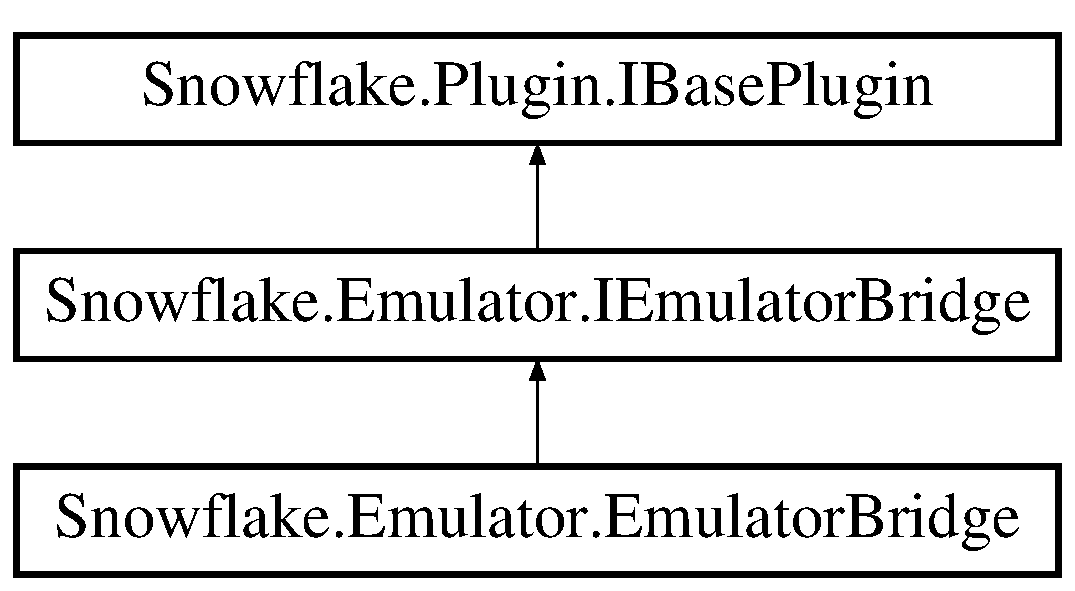
\includegraphics[height=3.000000cm]{interface_snowflake_1_1_emulator_1_1_i_emulator_bridge}
\end{center}
\end{figure}
\subsection*{Public Member Functions}
\begin{DoxyCompactItemize}
\item 
\hypertarget{interface_snowflake_1_1_emulator_1_1_i_emulator_bridge_a8245f048054db9e2b45f07bebaea3c02}{}void {\bfseries Start\+Rom} (\hyperlink{interface_snowflake_1_1_game_1_1_i_game_info}{I\+Game\+Info} game\+Info)\label{interface_snowflake_1_1_emulator_1_1_i_emulator_bridge_a8245f048054db9e2b45f07bebaea3c02}

\item 
\hypertarget{interface_snowflake_1_1_emulator_1_1_i_emulator_bridge_ad66a4b4654ef5856ee6393145b36f666}{}string {\bfseries Compile\+Configuration} (\hyperlink{interface_snowflake_1_1_emulator_1_1_configuration_1_1_i_configuration_profile}{I\+Configuration\+Profile} configuration\+Profile)\label{interface_snowflake_1_1_emulator_1_1_i_emulator_bridge_ad66a4b4654ef5856ee6393145b36f666}

\item 
\hypertarget{interface_snowflake_1_1_emulator_1_1_i_emulator_bridge_a55429243533cb5c9eb3ba204b73b4113}{}string {\bfseries Compile\+Configuration} (\hyperlink{interface_snowflake_1_1_emulator_1_1_configuration_1_1_i_configuration_template}{I\+Configuration\+Template} configuration\+Template, \hyperlink{interface_snowflake_1_1_emulator_1_1_configuration_1_1_i_configuration_profile}{I\+Configuration\+Profile} configuration\+Profile)\label{interface_snowflake_1_1_emulator_1_1_i_emulator_bridge_a55429243533cb5c9eb3ba204b73b4113}

\item 
\hypertarget{interface_snowflake_1_1_emulator_1_1_i_emulator_bridge_add8bb90ed261a06469c3bafbeeb4d7ab}{}string {\bfseries Compile\+Controller} (int player\+Index, \hyperlink{interface_snowflake_1_1_controller_1_1_i_controller_definition}{I\+Controller\+Definition} controller\+Definition, \hyperlink{interface_snowflake_1_1_emulator_1_1_input_1_1_i_controller_template}{I\+Controller\+Template} controller\+Template, \hyperlink{interface_snowflake_1_1_controller_1_1_i_controller_profile}{I\+Controller\+Profile} controller\+Profile, \hyperlink{interface_snowflake_1_1_emulator_1_1_input_1_1_i_input_template}{I\+Input\+Template} input\+Template)\label{interface_snowflake_1_1_emulator_1_1_i_emulator_bridge_add8bb90ed261a06469c3bafbeeb4d7ab}

\item 
\hypertarget{interface_snowflake_1_1_emulator_1_1_i_emulator_bridge_afddc96f9e6aab97573ea4eafb6498dad}{}string {\bfseries Compile\+Controller} (int player\+Index, \hyperlink{interface_snowflake_1_1_platform_1_1_i_platform_info}{I\+Platform\+Info} platform\+Info, \hyperlink{interface_snowflake_1_1_emulator_1_1_input_1_1_i_input_template}{I\+Input\+Template} input\+Template)\label{interface_snowflake_1_1_emulator_1_1_i_emulator_bridge_afddc96f9e6aab97573ea4eafb6498dad}

\item 
\hypertarget{interface_snowflake_1_1_emulator_1_1_i_emulator_bridge_a5e7b55a9d318399191fd8857aa163f8c}{}void {\bfseries Shutdown\+Emulator} ()\label{interface_snowflake_1_1_emulator_1_1_i_emulator_bridge_a5e7b55a9d318399191fd8857aa163f8c}

\item 
\hypertarget{interface_snowflake_1_1_emulator_1_1_i_emulator_bridge_ac88a67e269c1d31551e8c4c0bd315c0e}{}void {\bfseries Handle\+Prompt} (string prompt\+Message)\label{interface_snowflake_1_1_emulator_1_1_i_emulator_bridge_ac88a67e269c1d31551e8c4c0bd315c0e}

\end{DoxyCompactItemize}
\subsection*{Properties}
\begin{DoxyCompactItemize}
\item 
\hypertarget{interface_snowflake_1_1_emulator_1_1_i_emulator_bridge_a16b6fb49e7a8918e8008cf6a63c7ca61}{}\hyperlink{interface_snowflake_1_1_emulator_1_1_i_emulator_assembly}{I\+Emulator\+Assembly} {\bfseries Emulator\+Assembly}\hspace{0.3cm}{\ttfamily  \mbox{[}get\mbox{]}}\label{interface_snowflake_1_1_emulator_1_1_i_emulator_bridge_a16b6fb49e7a8918e8008cf6a63c7ca61}

\item 
\hypertarget{interface_snowflake_1_1_emulator_1_1_i_emulator_bridge_aa9202ffa8300af600ea2936307c58df8}{}I\+List$<$ string $>$ {\bfseries Supported\+Platforms}\hspace{0.3cm}{\ttfamily  \mbox{[}get\mbox{]}}\label{interface_snowflake_1_1_emulator_1_1_i_emulator_bridge_aa9202ffa8300af600ea2936307c58df8}

\item 
\hypertarget{interface_snowflake_1_1_emulator_1_1_i_emulator_bridge_a3230286b490dc33b3327b8a2a236b469}{}I\+Dictionary$<$ string, \hyperlink{interface_snowflake_1_1_emulator_1_1_input_1_1_i_controller_template}{I\+Controller\+Template} $>$ {\bfseries Controller\+Templates}\hspace{0.3cm}{\ttfamily  \mbox{[}get\mbox{]}}\label{interface_snowflake_1_1_emulator_1_1_i_emulator_bridge_a3230286b490dc33b3327b8a2a236b469}

\item 
\hypertarget{interface_snowflake_1_1_emulator_1_1_i_emulator_bridge_a9314563179c8ea7ff50bbf030c667ca8}{}I\+Dictionary$<$ string, \hyperlink{interface_snowflake_1_1_emulator_1_1_input_1_1_i_input_template}{I\+Input\+Template} $>$ {\bfseries Input\+Templates}\hspace{0.3cm}{\ttfamily  \mbox{[}get\mbox{]}}\label{interface_snowflake_1_1_emulator_1_1_i_emulator_bridge_a9314563179c8ea7ff50bbf030c667ca8}

\item 
\hypertarget{interface_snowflake_1_1_emulator_1_1_i_emulator_bridge_a58d58675778f25f34bcaa5cf512c60ae}{}I\+Dictionary$<$ string, \hyperlink{interface_snowflake_1_1_emulator_1_1_configuration_1_1_i_configuration_template}{I\+Configuration\+Template} $>$ {\bfseries Configuration\+Templates}\hspace{0.3cm}{\ttfamily  \mbox{[}get\mbox{]}}\label{interface_snowflake_1_1_emulator_1_1_i_emulator_bridge_a58d58675778f25f34bcaa5cf512c60ae}

\end{DoxyCompactItemize}


The documentation for this interface was generated from the following file\+:\begin{DoxyCompactItemize}
\item 
Emulator/I\+Emulator\+Bridge.\+cs\end{DoxyCompactItemize}

\hypertarget{interface_snowflake_1_1_game_1_1_i_game_database}{}\section{Snowflake.\+Game.\+I\+Game\+Database Interface Reference}
\label{interface_snowflake_1_1_game_1_1_i_game_database}\index{Snowflake.\+Game.\+I\+Game\+Database@{Snowflake.\+Game.\+I\+Game\+Database}}


A database used to store game information  


\subsection*{Public Member Functions}
\begin{DoxyCompactItemize}
\item 
void \hyperlink{interface_snowflake_1_1_game_1_1_i_game_database_ac3df9a6fa7133f65296dfc500d545083}{Add\+Game} (\hyperlink{interface_snowflake_1_1_game_1_1_i_game_info}{I\+Game\+Info} game)
\begin{DoxyCompactList}\small\item\em Add a game to the database \end{DoxyCompactList}\item 
I\+List$<$ \hyperlink{interface_snowflake_1_1_game_1_1_i_game_info}{I\+Game\+Info} $>$ \hyperlink{interface_snowflake_1_1_game_1_1_i_game_database_a3584894d7c51710b8f0798ea2c37627e}{Get\+All\+Games} ()
\begin{DoxyCompactList}\small\item\em Get a list of all games in the database \end{DoxyCompactList}\item 
\hyperlink{interface_snowflake_1_1_game_1_1_i_game_info}{I\+Game\+Info} \hyperlink{interface_snowflake_1_1_game_1_1_i_game_database_aef05226f448d26158878e2b3e9174600}{Get\+Game\+By\+U\+U\+I\+D} (string uuid)
\begin{DoxyCompactList}\small\item\em Gets a game by it\textquotesingle{}s unique id \end{DoxyCompactList}\item 
I\+List$<$ \hyperlink{interface_snowflake_1_1_game_1_1_i_game_info}{I\+Game\+Info} $>$ \hyperlink{interface_snowflake_1_1_game_1_1_i_game_database_a020cfc0c7185c730e072bb2488871c6f}{Get\+Games\+By\+Name} (string name\+Search)
\begin{DoxyCompactList}\small\item\em Gets a list of games with a certain matching name \end{DoxyCompactList}\item 
I\+List$<$ \hyperlink{interface_snowflake_1_1_game_1_1_i_game_info}{I\+Game\+Info} $>$ \hyperlink{interface_snowflake_1_1_game_1_1_i_game_database_a8be96dda13fe81e23d35dbb0e50a36e0}{Get\+Games\+By\+Platform} (string platform\+Id)
\begin{DoxyCompactList}\small\item\em Gets all the games for a certain platform \end{DoxyCompactList}\end{DoxyCompactItemize}


\subsection{Detailed Description}
A database used to store game information 



\subsection{Member Function Documentation}
\hypertarget{interface_snowflake_1_1_game_1_1_i_game_database_ac3df9a6fa7133f65296dfc500d545083}{}\index{Snowflake\+::\+Game\+::\+I\+Game\+Database@{Snowflake\+::\+Game\+::\+I\+Game\+Database}!Add\+Game@{Add\+Game}}
\index{Add\+Game@{Add\+Game}!Snowflake\+::\+Game\+::\+I\+Game\+Database@{Snowflake\+::\+Game\+::\+I\+Game\+Database}}
\subsubsection[{Add\+Game}]{\setlength{\rightskip}{0pt plus 5cm}void Snowflake.\+Game.\+I\+Game\+Database.\+Add\+Game (
\begin{DoxyParamCaption}
\item[{{\bf I\+Game\+Info}}]{game}
\end{DoxyParamCaption}
)}\label{interface_snowflake_1_1_game_1_1_i_game_database_ac3df9a6fa7133f65296dfc500d545083}


Add a game to the database 


\begin{DoxyParams}{Parameters}
{\em game} & The game to add\\
\hline
\end{DoxyParams}
\hypertarget{interface_snowflake_1_1_game_1_1_i_game_database_a3584894d7c51710b8f0798ea2c37627e}{}\index{Snowflake\+::\+Game\+::\+I\+Game\+Database@{Snowflake\+::\+Game\+::\+I\+Game\+Database}!Get\+All\+Games@{Get\+All\+Games}}
\index{Get\+All\+Games@{Get\+All\+Games}!Snowflake\+::\+Game\+::\+I\+Game\+Database@{Snowflake\+::\+Game\+::\+I\+Game\+Database}}
\subsubsection[{Get\+All\+Games}]{\setlength{\rightskip}{0pt plus 5cm}I\+List$<${\bf I\+Game\+Info}$>$ Snowflake.\+Game.\+I\+Game\+Database.\+Get\+All\+Games (
\begin{DoxyParamCaption}
{}
\end{DoxyParamCaption}
)}\label{interface_snowflake_1_1_game_1_1_i_game_database_a3584894d7c51710b8f0798ea2c37627e}


Get a list of all games in the database 

\begin{DoxyReturn}{Returns}
A list of all games in the database
\end{DoxyReturn}
\hypertarget{interface_snowflake_1_1_game_1_1_i_game_database_aef05226f448d26158878e2b3e9174600}{}\index{Snowflake\+::\+Game\+::\+I\+Game\+Database@{Snowflake\+::\+Game\+::\+I\+Game\+Database}!Get\+Game\+By\+U\+U\+I\+D@{Get\+Game\+By\+U\+U\+I\+D}}
\index{Get\+Game\+By\+U\+U\+I\+D@{Get\+Game\+By\+U\+U\+I\+D}!Snowflake\+::\+Game\+::\+I\+Game\+Database@{Snowflake\+::\+Game\+::\+I\+Game\+Database}}
\subsubsection[{Get\+Game\+By\+U\+U\+I\+D}]{\setlength{\rightskip}{0pt plus 5cm}{\bf I\+Game\+Info} Snowflake.\+Game.\+I\+Game\+Database.\+Get\+Game\+By\+U\+U\+I\+D (
\begin{DoxyParamCaption}
\item[{string}]{uuid}
\end{DoxyParamCaption}
)}\label{interface_snowflake_1_1_game_1_1_i_game_database_aef05226f448d26158878e2b3e9174600}


Gets a game by it\textquotesingle{}s unique id 


\begin{DoxyParams}{Parameters}
{\em uuid} & The unique id of the game\\
\hline
\end{DoxyParams}
\begin{DoxyReturn}{Returns}
The game with the unique id
\end{DoxyReturn}
\hypertarget{interface_snowflake_1_1_game_1_1_i_game_database_a020cfc0c7185c730e072bb2488871c6f}{}\index{Snowflake\+::\+Game\+::\+I\+Game\+Database@{Snowflake\+::\+Game\+::\+I\+Game\+Database}!Get\+Games\+By\+Name@{Get\+Games\+By\+Name}}
\index{Get\+Games\+By\+Name@{Get\+Games\+By\+Name}!Snowflake\+::\+Game\+::\+I\+Game\+Database@{Snowflake\+::\+Game\+::\+I\+Game\+Database}}
\subsubsection[{Get\+Games\+By\+Name}]{\setlength{\rightskip}{0pt plus 5cm}I\+List$<${\bf I\+Game\+Info}$>$ Snowflake.\+Game.\+I\+Game\+Database.\+Get\+Games\+By\+Name (
\begin{DoxyParamCaption}
\item[{string}]{name\+Search}
\end{DoxyParamCaption}
)}\label{interface_snowflake_1_1_game_1_1_i_game_database_a020cfc0c7185c730e072bb2488871c6f}


Gets a list of games with a certain matching name 


\begin{DoxyParams}{Parameters}
{\em name\+Search} & The name of the game to search by\\
\hline
\end{DoxyParams}
\begin{DoxyReturn}{Returns}
A list of games with matching titles
\end{DoxyReturn}
\hypertarget{interface_snowflake_1_1_game_1_1_i_game_database_a8be96dda13fe81e23d35dbb0e50a36e0}{}\index{Snowflake\+::\+Game\+::\+I\+Game\+Database@{Snowflake\+::\+Game\+::\+I\+Game\+Database}!Get\+Games\+By\+Platform@{Get\+Games\+By\+Platform}}
\index{Get\+Games\+By\+Platform@{Get\+Games\+By\+Platform}!Snowflake\+::\+Game\+::\+I\+Game\+Database@{Snowflake\+::\+Game\+::\+I\+Game\+Database}}
\subsubsection[{Get\+Games\+By\+Platform}]{\setlength{\rightskip}{0pt plus 5cm}I\+List$<${\bf I\+Game\+Info}$>$ Snowflake.\+Game.\+I\+Game\+Database.\+Get\+Games\+By\+Platform (
\begin{DoxyParamCaption}
\item[{string}]{platform\+Id}
\end{DoxyParamCaption}
)}\label{interface_snowflake_1_1_game_1_1_i_game_database_a8be96dda13fe81e23d35dbb0e50a36e0}


Gets all the games for a certain platform 


\begin{DoxyParams}{Parameters}
{\em platform\+Id} & The platform id to search for\\
\hline
\end{DoxyParams}
\begin{DoxyReturn}{Returns}
All games in a certain platform
\end{DoxyReturn}


The documentation for this interface was generated from the following file\+:\begin{DoxyCompactItemize}
\item 
Game/I\+Game\+Database.\+cs\end{DoxyCompactItemize}

\hypertarget{interface_snowflake_1_1_scraper_1_1_i_game_images_result}{}\section{Snowflake.\+Scraper.\+I\+Game\+Images\+Result Interface Reference}
\label{interface_snowflake_1_1_scraper_1_1_i_game_images_result}\index{Snowflake.\+Scraper.\+I\+Game\+Images\+Result@{Snowflake.\+Scraper.\+I\+Game\+Images\+Result}}
\subsection*{Public Member Functions}
\begin{DoxyCompactItemize}
\item 
\hypertarget{interface_snowflake_1_1_scraper_1_1_i_game_images_result_adf40922df33f6064d2eda4ec51956c54}{}void {\bfseries Add\+From\+Url} (Game\+Image\+Type image\+Type, Uri image\+Url)\label{interface_snowflake_1_1_scraper_1_1_i_game_images_result_adf40922df33f6064d2eda4ec51956c54}

\item 
\hypertarget{interface_snowflake_1_1_scraper_1_1_i_game_images_result_affeeec97c8d5228b7d05b1bcae9761d0}{}\hyperlink{interface_snowflake_1_1_information_1_1_media_store_1_1_i_media_store}{I\+Media\+Store} {\bfseries To\+Media\+Store} (string media\+Store\+Key)\label{interface_snowflake_1_1_scraper_1_1_i_game_images_result_affeeec97c8d5228b7d05b1bcae9761d0}

\end{DoxyCompactItemize}
\subsection*{Properties}
\begin{DoxyCompactItemize}
\item 
\hypertarget{interface_snowflake_1_1_scraper_1_1_i_game_images_result_a43e549bdb8262de9312dbbec70cffe7b}{}I\+Dictionary$<$ string, string $>$ {\bfseries Boxarts}\hspace{0.3cm}{\ttfamily  \mbox{[}get, set\mbox{]}}\label{interface_snowflake_1_1_scraper_1_1_i_game_images_result_a43e549bdb8262de9312dbbec70cffe7b}

\item 
\hypertarget{interface_snowflake_1_1_scraper_1_1_i_game_images_result_a1e72093bed4ba6e5649032e048d6a4ee}{}I\+List$<$ string $>$ {\bfseries Fanarts}\hspace{0.3cm}{\ttfamily  \mbox{[}get, set\mbox{]}}\label{interface_snowflake_1_1_scraper_1_1_i_game_images_result_a1e72093bed4ba6e5649032e048d6a4ee}

\item 
\hypertarget{interface_snowflake_1_1_scraper_1_1_i_game_images_result_a3a2c0cb208cd30a431a8493cc7589cb1}{}string {\bfseries Images\+I\+D}\hspace{0.3cm}{\ttfamily  \mbox{[}get\mbox{]}}\label{interface_snowflake_1_1_scraper_1_1_i_game_images_result_a3a2c0cb208cd30a431a8493cc7589cb1}

\item 
\hypertarget{interface_snowflake_1_1_scraper_1_1_i_game_images_result_adab7285230c4c88d2a38dbd0d4921085}{}I\+List$<$ string $>$ {\bfseries Screenshots}\hspace{0.3cm}{\ttfamily  \mbox{[}get, set\mbox{]}}\label{interface_snowflake_1_1_scraper_1_1_i_game_images_result_adab7285230c4c88d2a38dbd0d4921085}

\end{DoxyCompactItemize}


The documentation for this interface was generated from the following file\+:\begin{DoxyCompactItemize}
\item 
Scraper/I\+Game\+Images\+Result.\+cs\end{DoxyCompactItemize}

\hypertarget{interface_snowflake_1_1_game_1_1_i_game_info}{}\section{Snowflake.\+Game.\+I\+Game\+Info Interface Reference}
\label{interface_snowflake_1_1_game_1_1_i_game_info}\index{Snowflake.\+Game.\+I\+Game\+Info@{Snowflake.\+Game.\+I\+Game\+Info}}
Inheritance diagram for Snowflake.\+Game.\+I\+Game\+Info\+:\begin{figure}[H]
\begin{center}
\leavevmode
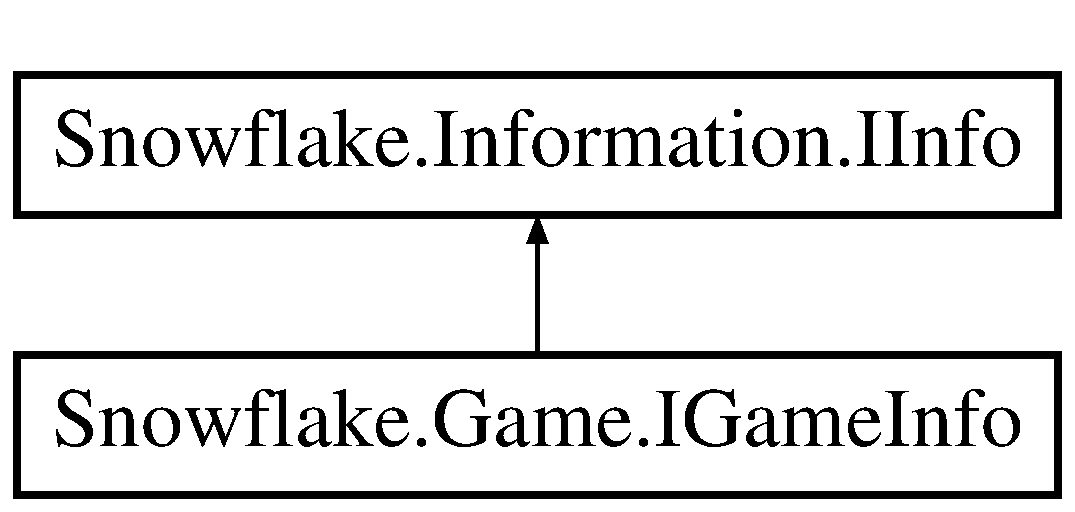
\includegraphics[height=2.000000cm]{interface_snowflake_1_1_game_1_1_i_game_info}
\end{center}
\end{figure}
\subsection*{Properties}
\begin{DoxyCompactItemize}
\item 
\hypertarget{interface_snowflake_1_1_game_1_1_i_game_info_a9a22682d66d9686ff4d64e83eb961624}{}string {\bfseries C\+R\+C32}\hspace{0.3cm}{\ttfamily  \mbox{[}get\mbox{]}}\label{interface_snowflake_1_1_game_1_1_i_game_info_a9a22682d66d9686ff4d64e83eb961624}

\item 
\hypertarget{interface_snowflake_1_1_game_1_1_i_game_info_a9d47fb0690eb47f4bdf2e0e60afc4555}{}string {\bfseries File\+Name}\hspace{0.3cm}{\ttfamily  \mbox{[}get\mbox{]}}\label{interface_snowflake_1_1_game_1_1_i_game_info_a9d47fb0690eb47f4bdf2e0e60afc4555}

\item 
\hypertarget{interface_snowflake_1_1_game_1_1_i_game_info_ad1ce0e9aece31e7b1f38f867177e7bee}{}string {\bfseries U\+U\+I\+D}\hspace{0.3cm}{\ttfamily  \mbox{[}get\mbox{]}}\label{interface_snowflake_1_1_game_1_1_i_game_info_ad1ce0e9aece31e7b1f38f867177e7bee}

\end{DoxyCompactItemize}


The documentation for this interface was generated from the following file\+:\begin{DoxyCompactItemize}
\item 
Game/I\+Game\+Info.\+cs\end{DoxyCompactItemize}

\hypertarget{interface_snowflake_1_1_emulator_1_1_input_1_1_i_gamepad_mapping}{}\section{Snowflake.\+Emulator.\+Input.\+I\+Gamepad\+Mapping Interface Reference}
\label{interface_snowflake_1_1_emulator_1_1_input_1_1_i_gamepad_mapping}\index{Snowflake.\+Emulator.\+Input.\+I\+Gamepad\+Mapping@{Snowflake.\+Emulator.\+Input.\+I\+Gamepad\+Mapping}}
\subsection*{Properties}
\begin{DoxyCompactItemize}
\item 
\hypertarget{interface_snowflake_1_1_emulator_1_1_input_1_1_i_gamepad_mapping_af59588b20b95d350a75333a38574e3f3}{}string {\bfseries G\+A\+M\+E\+P\+A\+D\+\_\+\+A}\hspace{0.3cm}{\ttfamily  \mbox{[}get\mbox{]}}\label{interface_snowflake_1_1_emulator_1_1_input_1_1_i_gamepad_mapping_af59588b20b95d350a75333a38574e3f3}

\item 
\hypertarget{interface_snowflake_1_1_emulator_1_1_input_1_1_i_gamepad_mapping_a9bed1e2f3e80c3bc43888fc7b0107483}{}string {\bfseries G\+A\+M\+E\+P\+A\+D\+\_\+\+B}\hspace{0.3cm}{\ttfamily  \mbox{[}get\mbox{]}}\label{interface_snowflake_1_1_emulator_1_1_input_1_1_i_gamepad_mapping_a9bed1e2f3e80c3bc43888fc7b0107483}

\item 
\hypertarget{interface_snowflake_1_1_emulator_1_1_input_1_1_i_gamepad_mapping_a8021f81f230312a13fb1de108c5ad252}{}string {\bfseries G\+A\+M\+E\+P\+A\+D\+\_\+\+D\+P\+A\+D\+\_\+\+D\+O\+W\+N}\hspace{0.3cm}{\ttfamily  \mbox{[}get\mbox{]}}\label{interface_snowflake_1_1_emulator_1_1_input_1_1_i_gamepad_mapping_a8021f81f230312a13fb1de108c5ad252}

\item 
\hypertarget{interface_snowflake_1_1_emulator_1_1_input_1_1_i_gamepad_mapping_a9e07f64a2ddb30be0994d36b9c44526d}{}string {\bfseries G\+A\+M\+E\+P\+A\+D\+\_\+\+D\+P\+A\+D\+\_\+\+L\+E\+F\+T}\hspace{0.3cm}{\ttfamily  \mbox{[}get\mbox{]}}\label{interface_snowflake_1_1_emulator_1_1_input_1_1_i_gamepad_mapping_a9e07f64a2ddb30be0994d36b9c44526d}

\item 
\hypertarget{interface_snowflake_1_1_emulator_1_1_input_1_1_i_gamepad_mapping_a967dd3c71e7a43aa1b8cd4af2fe45c9d}{}string {\bfseries G\+A\+M\+E\+P\+A\+D\+\_\+\+D\+P\+A\+D\+\_\+\+R\+I\+G\+H\+T}\hspace{0.3cm}{\ttfamily  \mbox{[}get\mbox{]}}\label{interface_snowflake_1_1_emulator_1_1_input_1_1_i_gamepad_mapping_a967dd3c71e7a43aa1b8cd4af2fe45c9d}

\item 
\hypertarget{interface_snowflake_1_1_emulator_1_1_input_1_1_i_gamepad_mapping_a27f5c43113d5787424ae98a4a0f94ff8}{}string {\bfseries G\+A\+M\+E\+P\+A\+D\+\_\+\+D\+P\+A\+D\+\_\+\+U\+P}\hspace{0.3cm}{\ttfamily  \mbox{[}get\mbox{]}}\label{interface_snowflake_1_1_emulator_1_1_input_1_1_i_gamepad_mapping_a27f5c43113d5787424ae98a4a0f94ff8}

\item 
\hypertarget{interface_snowflake_1_1_emulator_1_1_input_1_1_i_gamepad_mapping_aa415033cdebdccc2ecf6240d98788e46}{}string {\bfseries G\+A\+M\+E\+P\+A\+D\+\_\+\+G\+U\+I\+D\+E}\hspace{0.3cm}{\ttfamily  \mbox{[}get\mbox{]}}\label{interface_snowflake_1_1_emulator_1_1_input_1_1_i_gamepad_mapping_aa415033cdebdccc2ecf6240d98788e46}

\item 
\hypertarget{interface_snowflake_1_1_emulator_1_1_input_1_1_i_gamepad_mapping_a33b71e9b671c6b389fbf39514a2fcc2d}{}string {\bfseries G\+A\+M\+E\+P\+A\+D\+\_\+\+L\+\_\+\+X\+\_\+\+D\+O\+W\+N}\hspace{0.3cm}{\ttfamily  \mbox{[}get\mbox{]}}\label{interface_snowflake_1_1_emulator_1_1_input_1_1_i_gamepad_mapping_a33b71e9b671c6b389fbf39514a2fcc2d}

\item 
\hypertarget{interface_snowflake_1_1_emulator_1_1_input_1_1_i_gamepad_mapping_abbec65db792c3d55abfa830a55777fe3}{}string {\bfseries G\+A\+M\+E\+P\+A\+D\+\_\+\+L\+\_\+\+X\+\_\+\+U\+P}\hspace{0.3cm}{\ttfamily  \mbox{[}get\mbox{]}}\label{interface_snowflake_1_1_emulator_1_1_input_1_1_i_gamepad_mapping_abbec65db792c3d55abfa830a55777fe3}

\item 
\hypertarget{interface_snowflake_1_1_emulator_1_1_input_1_1_i_gamepad_mapping_af771fd98a92c7bf1158e29612c3cc7a8}{}string {\bfseries G\+A\+M\+E\+P\+A\+D\+\_\+\+L\+\_\+\+Y\+\_\+\+L\+E\+F\+T}\hspace{0.3cm}{\ttfamily  \mbox{[}get\mbox{]}}\label{interface_snowflake_1_1_emulator_1_1_input_1_1_i_gamepad_mapping_af771fd98a92c7bf1158e29612c3cc7a8}

\item 
\hypertarget{interface_snowflake_1_1_emulator_1_1_input_1_1_i_gamepad_mapping_aa10ecb4659c58815773ab2b9c7897ea2}{}string {\bfseries G\+A\+M\+E\+P\+A\+D\+\_\+\+L\+\_\+\+Y\+\_\+\+R\+I\+G\+H\+T}\hspace{0.3cm}{\ttfamily  \mbox{[}get\mbox{]}}\label{interface_snowflake_1_1_emulator_1_1_input_1_1_i_gamepad_mapping_aa10ecb4659c58815773ab2b9c7897ea2}

\item 
\hypertarget{interface_snowflake_1_1_emulator_1_1_input_1_1_i_gamepad_mapping_acd484a2c007414aa1301a89aa4b651be}{}string {\bfseries G\+A\+M\+E\+P\+A\+D\+\_\+\+L1}\hspace{0.3cm}{\ttfamily  \mbox{[}get\mbox{]}}\label{interface_snowflake_1_1_emulator_1_1_input_1_1_i_gamepad_mapping_acd484a2c007414aa1301a89aa4b651be}

\item 
\hypertarget{interface_snowflake_1_1_emulator_1_1_input_1_1_i_gamepad_mapping_ae5b185725683a8477a89b56b08114cee}{}string {\bfseries G\+A\+M\+E\+P\+A\+D\+\_\+\+L2}\hspace{0.3cm}{\ttfamily  \mbox{[}get\mbox{]}}\label{interface_snowflake_1_1_emulator_1_1_input_1_1_i_gamepad_mapping_ae5b185725683a8477a89b56b08114cee}

\item 
\hypertarget{interface_snowflake_1_1_emulator_1_1_input_1_1_i_gamepad_mapping_a8df3594e24dc099ae41a46b8bd80cf09}{}string {\bfseries G\+A\+M\+E\+P\+A\+D\+\_\+\+L3}\hspace{0.3cm}{\ttfamily  \mbox{[}get\mbox{]}}\label{interface_snowflake_1_1_emulator_1_1_input_1_1_i_gamepad_mapping_a8df3594e24dc099ae41a46b8bd80cf09}

\item 
\hypertarget{interface_snowflake_1_1_emulator_1_1_input_1_1_i_gamepad_mapping_acc2fc81e6b53d28e5406f410a74448e5}{}string {\bfseries G\+A\+M\+E\+P\+A\+D\+\_\+\+R\+\_\+\+X\+\_\+\+D\+O\+W\+N}\hspace{0.3cm}{\ttfamily  \mbox{[}get\mbox{]}}\label{interface_snowflake_1_1_emulator_1_1_input_1_1_i_gamepad_mapping_acc2fc81e6b53d28e5406f410a74448e5}

\item 
\hypertarget{interface_snowflake_1_1_emulator_1_1_input_1_1_i_gamepad_mapping_a6f58d12ed78fca0358f24db7fbcaae17}{}string {\bfseries G\+A\+M\+E\+P\+A\+D\+\_\+\+R\+\_\+\+X\+\_\+\+U\+P}\hspace{0.3cm}{\ttfamily  \mbox{[}get\mbox{]}}\label{interface_snowflake_1_1_emulator_1_1_input_1_1_i_gamepad_mapping_a6f58d12ed78fca0358f24db7fbcaae17}

\item 
\hypertarget{interface_snowflake_1_1_emulator_1_1_input_1_1_i_gamepad_mapping_ab54e9e680679ef97bcfa9d6c855e55ee}{}string {\bfseries G\+A\+M\+E\+P\+A\+D\+\_\+\+R\+\_\+\+Y\+\_\+\+L\+E\+F\+T}\hspace{0.3cm}{\ttfamily  \mbox{[}get\mbox{]}}\label{interface_snowflake_1_1_emulator_1_1_input_1_1_i_gamepad_mapping_ab54e9e680679ef97bcfa9d6c855e55ee}

\item 
\hypertarget{interface_snowflake_1_1_emulator_1_1_input_1_1_i_gamepad_mapping_a442d8e9b8bed606be70dedb078963fc0}{}string {\bfseries G\+A\+M\+E\+P\+A\+D\+\_\+\+R\+\_\+\+Y\+\_\+\+R\+I\+G\+H\+T}\hspace{0.3cm}{\ttfamily  \mbox{[}get\mbox{]}}\label{interface_snowflake_1_1_emulator_1_1_input_1_1_i_gamepad_mapping_a442d8e9b8bed606be70dedb078963fc0}

\item 
\hypertarget{interface_snowflake_1_1_emulator_1_1_input_1_1_i_gamepad_mapping_afd64b6f8b5d992d4a35f0ca3a19edac3}{}string {\bfseries G\+A\+M\+E\+P\+A\+D\+\_\+\+R1}\hspace{0.3cm}{\ttfamily  \mbox{[}get\mbox{]}}\label{interface_snowflake_1_1_emulator_1_1_input_1_1_i_gamepad_mapping_afd64b6f8b5d992d4a35f0ca3a19edac3}

\item 
\hypertarget{interface_snowflake_1_1_emulator_1_1_input_1_1_i_gamepad_mapping_a2e8324e4aead6bc7b276bdf5911cf44f}{}string {\bfseries G\+A\+M\+E\+P\+A\+D\+\_\+\+R2}\hspace{0.3cm}{\ttfamily  \mbox{[}get\mbox{]}}\label{interface_snowflake_1_1_emulator_1_1_input_1_1_i_gamepad_mapping_a2e8324e4aead6bc7b276bdf5911cf44f}

\item 
\hypertarget{interface_snowflake_1_1_emulator_1_1_input_1_1_i_gamepad_mapping_ab9701d9bbceeddb709ac4afa26518a99}{}string {\bfseries G\+A\+M\+E\+P\+A\+D\+\_\+\+R3}\hspace{0.3cm}{\ttfamily  \mbox{[}get\mbox{]}}\label{interface_snowflake_1_1_emulator_1_1_input_1_1_i_gamepad_mapping_ab9701d9bbceeddb709ac4afa26518a99}

\item 
\hypertarget{interface_snowflake_1_1_emulator_1_1_input_1_1_i_gamepad_mapping_a297d4714c484feee1a30bed48a939208}{}string {\bfseries G\+A\+M\+E\+P\+A\+D\+\_\+\+S\+E\+L\+E\+C\+T}\hspace{0.3cm}{\ttfamily  \mbox{[}get\mbox{]}}\label{interface_snowflake_1_1_emulator_1_1_input_1_1_i_gamepad_mapping_a297d4714c484feee1a30bed48a939208}

\item 
\hypertarget{interface_snowflake_1_1_emulator_1_1_input_1_1_i_gamepad_mapping_aecb910dcabbba76d087f346e9f643dd5}{}string {\bfseries G\+A\+M\+E\+P\+A\+D\+\_\+\+S\+T\+A\+R\+T}\hspace{0.3cm}{\ttfamily  \mbox{[}get\mbox{]}}\label{interface_snowflake_1_1_emulator_1_1_input_1_1_i_gamepad_mapping_aecb910dcabbba76d087f346e9f643dd5}

\item 
\hypertarget{interface_snowflake_1_1_emulator_1_1_input_1_1_i_gamepad_mapping_a504dd81ab33d335b8577be71523e9743}{}string {\bfseries G\+A\+M\+E\+P\+A\+D\+\_\+\+X}\hspace{0.3cm}{\ttfamily  \mbox{[}get\mbox{]}}\label{interface_snowflake_1_1_emulator_1_1_input_1_1_i_gamepad_mapping_a504dd81ab33d335b8577be71523e9743}

\item 
\hypertarget{interface_snowflake_1_1_emulator_1_1_input_1_1_i_gamepad_mapping_abfef9537c03817def41c6401027cdca5}{}string {\bfseries G\+A\+M\+E\+P\+A\+D\+\_\+\+Y}\hspace{0.3cm}{\ttfamily  \mbox{[}get\mbox{]}}\label{interface_snowflake_1_1_emulator_1_1_input_1_1_i_gamepad_mapping_abfef9537c03817def41c6401027cdca5}

\item 
\hypertarget{interface_snowflake_1_1_emulator_1_1_input_1_1_i_gamepad_mapping_a203e65ccf8e6d672150df9d9d58ddd9e}{}string {\bfseries this\mbox{[}string key\mbox{]}}\hspace{0.3cm}{\ttfamily  \mbox{[}get\mbox{]}}\label{interface_snowflake_1_1_emulator_1_1_input_1_1_i_gamepad_mapping_a203e65ccf8e6d672150df9d9d58ddd9e}

\end{DoxyCompactItemize}


The documentation for this interface was generated from the following file\+:\begin{DoxyCompactItemize}
\item 
Emulator/\+Input/I\+Gamepad\+Mapping.\+cs\end{DoxyCompactItemize}

\hypertarget{interface_snowflake_1_1_scraper_1_1_i_game_scrape_result}{}\section{Snowflake.\+Scraper.\+I\+Game\+Scrape\+Result Interface Reference}
\label{interface_snowflake_1_1_scraper_1_1_i_game_scrape_result}\index{Snowflake.\+Scraper.\+I\+Game\+Scrape\+Result@{Snowflake.\+Scraper.\+I\+Game\+Scrape\+Result}}
\subsection*{Properties}
\begin{DoxyCompactItemize}
\item 
\hypertarget{interface_snowflake_1_1_scraper_1_1_i_game_scrape_result_a4f50b5cc838d753c900b2be5562c2b8c}{}string {\bfseries Game\+Title}\hspace{0.3cm}{\ttfamily  \mbox{[}get\mbox{]}}\label{interface_snowflake_1_1_scraper_1_1_i_game_scrape_result_a4f50b5cc838d753c900b2be5562c2b8c}

\item 
\hypertarget{interface_snowflake_1_1_scraper_1_1_i_game_scrape_result_afb1f9b93e49e8f00be08da0844d4259c}{}string {\bfseries I\+D}\hspace{0.3cm}{\ttfamily  \mbox{[}get\mbox{]}}\label{interface_snowflake_1_1_scraper_1_1_i_game_scrape_result_afb1f9b93e49e8f00be08da0844d4259c}

\item 
\hypertarget{interface_snowflake_1_1_scraper_1_1_i_game_scrape_result_a4afe93d0e4e63bc9584d7e1b2437d9b3}{}string {\bfseries Platform\+I\+D}\hspace{0.3cm}{\ttfamily  \mbox{[}get\mbox{]}}\label{interface_snowflake_1_1_scraper_1_1_i_game_scrape_result_a4afe93d0e4e63bc9584d7e1b2437d9b3}

\end{DoxyCompactItemize}


The documentation for this interface was generated from the following file\+:\begin{DoxyCompactItemize}
\item 
Scraper/I\+Game\+Scrape\+Result.\+cs\end{DoxyCompactItemize}

\hypertarget{interface_snowflake_1_1_plugin_1_1_i_general_plugin}{}\section{Snowflake.\+Plugin.\+I\+General\+Plugin Interface Reference}
\label{interface_snowflake_1_1_plugin_1_1_i_general_plugin}\index{Snowflake.\+Plugin.\+I\+General\+Plugin@{Snowflake.\+Plugin.\+I\+General\+Plugin}}
Inheritance diagram for Snowflake.\+Plugin.\+I\+General\+Plugin\+:\begin{figure}[H]
\begin{center}
\leavevmode
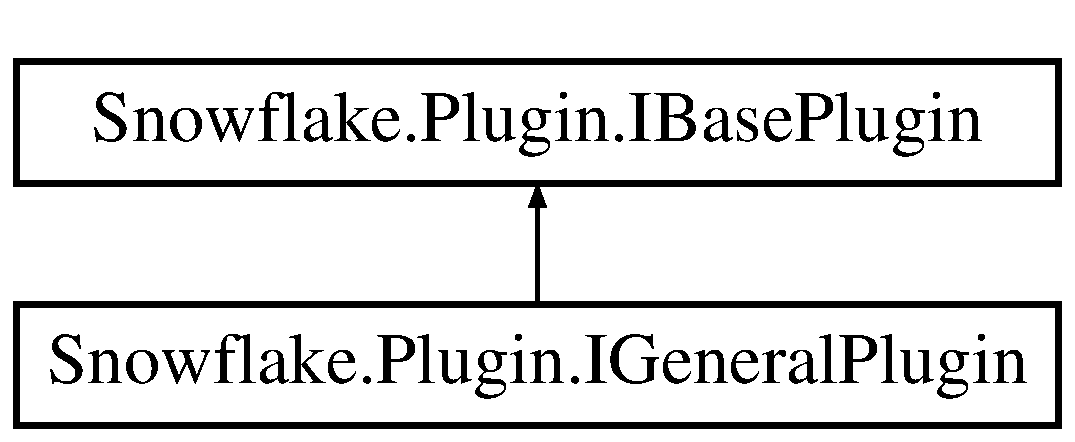
\includegraphics[height=2.000000cm]{interface_snowflake_1_1_plugin_1_1_i_general_plugin}
\end{center}
\end{figure}
\subsection*{Additional Inherited Members}


The documentation for this interface was generated from the following file\+:\begin{DoxyCompactItemize}
\item 
Plugin/I\+General\+Plugin.\+cs\end{DoxyCompactItemize}

\hypertarget{interface_snowflake_1_1_identifier_1_1_i_identifier}{}\section{Snowflake.\+Identifier.\+I\+Identifier Interface Reference}
\label{interface_snowflake_1_1_identifier_1_1_i_identifier}\index{Snowflake.\+Identifier.\+I\+Identifier@{Snowflake.\+Identifier.\+I\+Identifier}}
Inheritance diagram for Snowflake.\+Identifier.\+I\+Identifier\+:\begin{figure}[H]
\begin{center}
\leavevmode
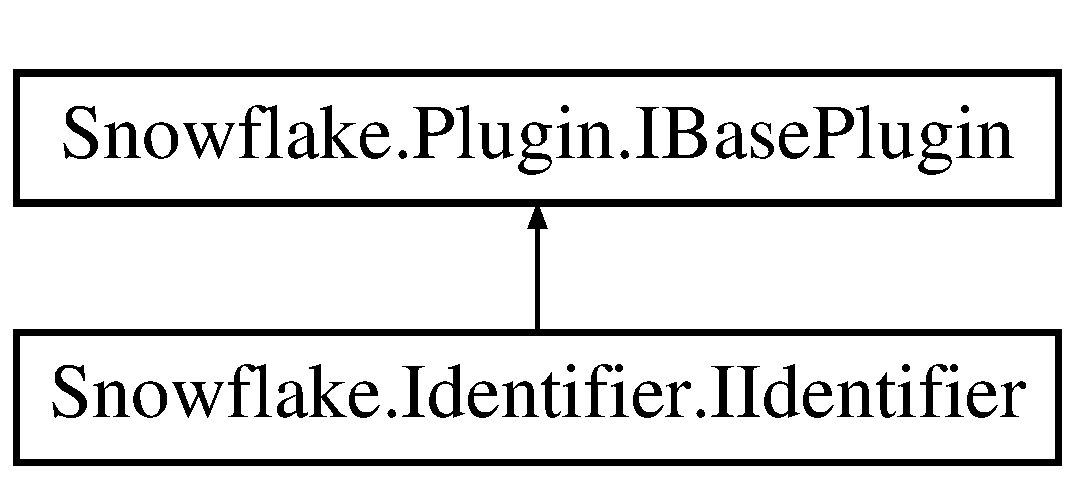
\includegraphics[height=2.000000cm]{interface_snowflake_1_1_identifier_1_1_i_identifier}
\end{center}
\end{figure}
\subsection*{Public Member Functions}
\begin{DoxyCompactItemize}
\item 
\hypertarget{interface_snowflake_1_1_identifier_1_1_i_identifier_a67579ab0b0467439f3381f9b2ce6ca6b}{}string {\bfseries Identify\+Game} (string file\+Name, string platform\+Id)\label{interface_snowflake_1_1_identifier_1_1_i_identifier_a67579ab0b0467439f3381f9b2ce6ca6b}

\item 
\hypertarget{interface_snowflake_1_1_identifier_1_1_i_identifier_ae2ebdad5be22c52be47ca198ac7aae21}{}string {\bfseries Identify\+Game} (File\+Stream file, string platform\+Id)\label{interface_snowflake_1_1_identifier_1_1_i_identifier_ae2ebdad5be22c52be47ca198ac7aae21}

\end{DoxyCompactItemize}
\subsection*{Additional Inherited Members}


The documentation for this interface was generated from the following file\+:\begin{DoxyCompactItemize}
\item 
Identifier/I\+Identifier.\+cs\end{DoxyCompactItemize}

\hypertarget{interface_snowflake_1_1_information_1_1_i_info}{}\section{Snowflake.\+Information.\+I\+Info Interface Reference}
\label{interface_snowflake_1_1_information_1_1_i_info}\index{Snowflake.\+Information.\+I\+Info@{Snowflake.\+Information.\+I\+Info}}
Inheritance diagram for Snowflake.\+Information.\+I\+Info\+:\begin{figure}[H]
\begin{center}
\leavevmode
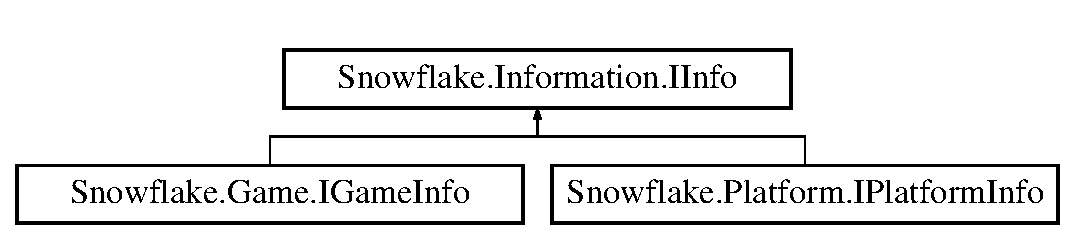
\includegraphics[height=2.000000cm]{interface_snowflake_1_1_information_1_1_i_info}
\end{center}
\end{figure}
\subsection*{Properties}
\begin{DoxyCompactItemize}
\item 
\hypertarget{interface_snowflake_1_1_information_1_1_i_info_adbca5b9f2db24b233866de3304500088}{}string {\bfseries Platform\+Id}\hspace{0.3cm}{\ttfamily  \mbox{[}get\mbox{]}}\label{interface_snowflake_1_1_information_1_1_i_info_adbca5b9f2db24b233866de3304500088}

\item 
\hypertarget{interface_snowflake_1_1_information_1_1_i_info_ad9450963e1d3443d2e5df274638fd8be}{}string {\bfseries Name}\hspace{0.3cm}{\ttfamily  \mbox{[}get\mbox{]}}\label{interface_snowflake_1_1_information_1_1_i_info_ad9450963e1d3443d2e5df274638fd8be}

\item 
\hypertarget{interface_snowflake_1_1_information_1_1_i_info_aeae6832deb9c513619b82c82ab94421c}{}I\+Dictionary$<$ string, string $>$ {\bfseries Metadata}\hspace{0.3cm}{\ttfamily  \mbox{[}get, set\mbox{]}}\label{interface_snowflake_1_1_information_1_1_i_info_aeae6832deb9c513619b82c82ab94421c}

\item 
\hypertarget{interface_snowflake_1_1_information_1_1_i_info_a871b33234ef2b413be1ee8e6846768b6}{}\hyperlink{interface_snowflake_1_1_information_1_1_media_store_1_1_i_media_store}{I\+Media\+Store} {\bfseries Media\+Store}\hspace{0.3cm}{\ttfamily  \mbox{[}get\mbox{]}}\label{interface_snowflake_1_1_information_1_1_i_info_a871b33234ef2b413be1ee8e6846768b6}

\end{DoxyCompactItemize}


The documentation for this interface was generated from the following file\+:\begin{DoxyCompactItemize}
\item 
Information/I\+Info.\+cs\end{DoxyCompactItemize}

\hypertarget{interface_snowflake_1_1_emulator_1_1_input_1_1_i_input_template}{}\section{Snowflake.\+Emulator.\+Input.\+I\+Input\+Template Interface Reference}
\label{interface_snowflake_1_1_emulator_1_1_input_1_1_i_input_template}\index{Snowflake.\+Emulator.\+Input.\+I\+Input\+Template@{Snowflake.\+Emulator.\+Input.\+I\+Input\+Template}}
\subsection*{Properties}
\begin{DoxyCompactItemize}
\item 
\hypertarget{interface_snowflake_1_1_emulator_1_1_input_1_1_i_input_template_ab8e0a7d250f6734b895cc62ef7bbe710}{}I\+Read\+Only\+Dictionary$<$ string, \hyperlink{interface_snowflake_1_1_emulator_1_1_input_1_1_i_gamepad_mapping}{I\+Gamepad\+Mapping} $>$ {\bfseries Gamepad\+Mappings}\hspace{0.3cm}{\ttfamily  \mbox{[}get\mbox{]}}\label{interface_snowflake_1_1_emulator_1_1_input_1_1_i_input_template_ab8e0a7d250f6734b895cc62ef7bbe710}

\item 
\hypertarget{interface_snowflake_1_1_emulator_1_1_input_1_1_i_input_template_a3e609bf0f4f4515ee91ea05f860f0211}{}I\+Read\+Only\+Dictionary$<$ string, \hyperlink{interface_snowflake_1_1_emulator_1_1_input_1_1_i_keyboard_mapping}{I\+Keyboard\+Mapping} $>$ {\bfseries Keyboard\+Mappings}\hspace{0.3cm}{\ttfamily  \mbox{[}get\mbox{]}}\label{interface_snowflake_1_1_emulator_1_1_input_1_1_i_input_template_a3e609bf0f4f4515ee91ea05f860f0211}

\item 
\hypertarget{interface_snowflake_1_1_emulator_1_1_input_1_1_i_input_template_a7495a77567b2cc97ecf959ed0f9dc4de}{}string {\bfseries No\+Bind}\hspace{0.3cm}{\ttfamily  \mbox{[}get\mbox{]}}\label{interface_snowflake_1_1_emulator_1_1_input_1_1_i_input_template_a7495a77567b2cc97ecf959ed0f9dc4de}

\item 
\hypertarget{interface_snowflake_1_1_emulator_1_1_input_1_1_i_input_template_a4771fa7fbc3f801990cf90a03185e010}{}string {\bfseries String\+Template}\hspace{0.3cm}{\ttfamily  \mbox{[}get\mbox{]}}\label{interface_snowflake_1_1_emulator_1_1_input_1_1_i_input_template_a4771fa7fbc3f801990cf90a03185e010}

\item 
\hypertarget{interface_snowflake_1_1_emulator_1_1_input_1_1_i_input_template_ae96998d9a6dc349e5e12f99d455465d4}{}I\+Read\+Only\+List$<$ string $>$ {\bfseries Template\+Keys}\hspace{0.3cm}{\ttfamily  \mbox{[}get\mbox{]}}\label{interface_snowflake_1_1_emulator_1_1_input_1_1_i_input_template_ae96998d9a6dc349e5e12f99d455465d4}

\end{DoxyCompactItemize}


The documentation for this interface was generated from the following file\+:\begin{DoxyCompactItemize}
\item 
Emulator/\+Input/I\+Input\+Template.\+cs\end{DoxyCompactItemize}

\hypertarget{interface_snowflake_1_1_ajax_1_1_i_j_s_request}{}\section{Snowflake.\+Ajax.\+I\+J\+S\+Request Interface Reference}
\label{interface_snowflake_1_1_ajax_1_1_i_j_s_request}\index{Snowflake.\+Ajax.\+I\+J\+S\+Request@{Snowflake.\+Ajax.\+I\+J\+S\+Request}}


Represents an \hyperlink{namespace_snowflake_1_1_ajax}{Ajax} Javascript Request  


\subsection*{Public Member Functions}
\begin{DoxyCompactItemize}
\item 
string \hyperlink{interface_snowflake_1_1_ajax_1_1_i_j_s_request_a68284d8affe41bd2f874d50c35718bf8}{Get\+Parameter} (string param\+Key)
\begin{DoxyCompactList}\small\item\em Gets a parameter from the request \end{DoxyCompactList}\end{DoxyCompactItemize}
\subsection*{Properties}
\begin{DoxyCompactItemize}
\item 
string \hyperlink{interface_snowflake_1_1_ajax_1_1_i_j_s_request_a89baf2c0eb864e3129b589a311dd12da}{Method\+Name}\hspace{0.3cm}{\ttfamily  \mbox{[}get\mbox{]}}
\begin{DoxyCompactList}\small\item\em The name of the method called \end{DoxyCompactList}\item 
I\+Dictionary$<$ string, string $>$ \hyperlink{interface_snowflake_1_1_ajax_1_1_i_j_s_request_a29b4147b39836395032254affd4fba95}{Method\+Parameters}\hspace{0.3cm}{\ttfamily  \mbox{[}get\mbox{]}}
\begin{DoxyCompactList}\small\item\em The method parameters the request was called with \end{DoxyCompactList}\item 
string \hyperlink{interface_snowflake_1_1_ajax_1_1_i_j_s_request_a0a45d83b00bed741f7c37220ac298bb8}{Name\+Space}\hspace{0.3cm}{\ttfamily  \mbox{[}get\mbox{]}}
\begin{DoxyCompactList}\small\item\em The Javascript namespace the called method belongs to \end{DoxyCompactList}\end{DoxyCompactItemize}


\subsection{Detailed Description}
Represents an \hyperlink{namespace_snowflake_1_1_ajax}{Ajax} Javascript Request 



\subsection{Member Function Documentation}
\hypertarget{interface_snowflake_1_1_ajax_1_1_i_j_s_request_a68284d8affe41bd2f874d50c35718bf8}{}\index{Snowflake\+::\+Ajax\+::\+I\+J\+S\+Request@{Snowflake\+::\+Ajax\+::\+I\+J\+S\+Request}!Get\+Parameter@{Get\+Parameter}}
\index{Get\+Parameter@{Get\+Parameter}!Snowflake\+::\+Ajax\+::\+I\+J\+S\+Request@{Snowflake\+::\+Ajax\+::\+I\+J\+S\+Request}}
\subsubsection[{Get\+Parameter}]{\setlength{\rightskip}{0pt plus 5cm}string Snowflake.\+Ajax.\+I\+J\+S\+Request.\+Get\+Parameter (
\begin{DoxyParamCaption}
\item[{string}]{param\+Key}
\end{DoxyParamCaption}
)}\label{interface_snowflake_1_1_ajax_1_1_i_j_s_request_a68284d8affe41bd2f874d50c35718bf8}


Gets a parameter from the request 


\begin{DoxyParams}{Parameters}
{\em param\+Key} & The parameter key\\
\hline
\end{DoxyParams}
\begin{DoxyReturn}{Returns}
The value of the parameter with the given key
\end{DoxyReturn}


\subsection{Property Documentation}
\hypertarget{interface_snowflake_1_1_ajax_1_1_i_j_s_request_a89baf2c0eb864e3129b589a311dd12da}{}\index{Snowflake\+::\+Ajax\+::\+I\+J\+S\+Request@{Snowflake\+::\+Ajax\+::\+I\+J\+S\+Request}!Method\+Name@{Method\+Name}}
\index{Method\+Name@{Method\+Name}!Snowflake\+::\+Ajax\+::\+I\+J\+S\+Request@{Snowflake\+::\+Ajax\+::\+I\+J\+S\+Request}}
\subsubsection[{Method\+Name}]{\setlength{\rightskip}{0pt plus 5cm}string Snowflake.\+Ajax.\+I\+J\+S\+Request.\+Method\+Name\hspace{0.3cm}{\ttfamily [get]}}\label{interface_snowflake_1_1_ajax_1_1_i_j_s_request_a89baf2c0eb864e3129b589a311dd12da}


The name of the method called 

\hypertarget{interface_snowflake_1_1_ajax_1_1_i_j_s_request_a29b4147b39836395032254affd4fba95}{}\index{Snowflake\+::\+Ajax\+::\+I\+J\+S\+Request@{Snowflake\+::\+Ajax\+::\+I\+J\+S\+Request}!Method\+Parameters@{Method\+Parameters}}
\index{Method\+Parameters@{Method\+Parameters}!Snowflake\+::\+Ajax\+::\+I\+J\+S\+Request@{Snowflake\+::\+Ajax\+::\+I\+J\+S\+Request}}
\subsubsection[{Method\+Parameters}]{\setlength{\rightskip}{0pt plus 5cm}I\+Dictionary$<$string, string$>$ Snowflake.\+Ajax.\+I\+J\+S\+Request.\+Method\+Parameters\hspace{0.3cm}{\ttfamily [get]}}\label{interface_snowflake_1_1_ajax_1_1_i_j_s_request_a29b4147b39836395032254affd4fba95}


The method parameters the request was called with 

\hypertarget{interface_snowflake_1_1_ajax_1_1_i_j_s_request_a0a45d83b00bed741f7c37220ac298bb8}{}\index{Snowflake\+::\+Ajax\+::\+I\+J\+S\+Request@{Snowflake\+::\+Ajax\+::\+I\+J\+S\+Request}!Name\+Space@{Name\+Space}}
\index{Name\+Space@{Name\+Space}!Snowflake\+::\+Ajax\+::\+I\+J\+S\+Request@{Snowflake\+::\+Ajax\+::\+I\+J\+S\+Request}}
\subsubsection[{Name\+Space}]{\setlength{\rightskip}{0pt plus 5cm}string Snowflake.\+Ajax.\+I\+J\+S\+Request.\+Name\+Space\hspace{0.3cm}{\ttfamily [get]}}\label{interface_snowflake_1_1_ajax_1_1_i_j_s_request_a0a45d83b00bed741f7c37220ac298bb8}


The Javascript namespace the called method belongs to 



The documentation for this interface was generated from the following file\+:\begin{DoxyCompactItemize}
\item 
Ajax/I\+J\+S\+Request.\+cs\end{DoxyCompactItemize}

\hypertarget{interface_snowflake_1_1_ajax_1_1_i_j_s_response}{}\section{Snowflake.\+Ajax.\+I\+J\+S\+Response Interface Reference}
\label{interface_snowflake_1_1_ajax_1_1_i_j_s_response}\index{Snowflake.\+Ajax.\+I\+J\+S\+Response@{Snowflake.\+Ajax.\+I\+J\+S\+Response}}


Represents a Javascript (J\+S\+O\+N) response to an A\+J\+A\+X request  


\subsection*{Public Member Functions}
\begin{DoxyCompactItemize}
\item 
string \hyperlink{interface_snowflake_1_1_ajax_1_1_i_j_s_response_aa48e2c58da48c0bc78308a51974fc34b}{Get\+Json} ()
\begin{DoxyCompactList}\small\item\em Gets a string representation of the generated J\+S\+O\+N with the provided response payload \end{DoxyCompactList}\end{DoxyCompactItemize}
\subsection*{Properties}
\begin{DoxyCompactItemize}
\item 
dynamic \hyperlink{interface_snowflake_1_1_ajax_1_1_i_j_s_response_aca4a568b350d1bcb3df0a5484e311670}{Payload}\hspace{0.3cm}{\ttfamily  \mbox{[}get\mbox{]}}
\begin{DoxyCompactList}\small\item\em The payload object to be returned to the request \end{DoxyCompactList}\item 
\hyperlink{interface_snowflake_1_1_ajax_1_1_i_j_s_request}{I\+J\+S\+Request} \hyperlink{interface_snowflake_1_1_ajax_1_1_i_j_s_response_ae35c86f83855bf0a8dcf50257b802b1e}{Request}\hspace{0.3cm}{\ttfamily  \mbox{[}get\mbox{]}}
\begin{DoxyCompactList}\small\item\em The A\+J\+A\+X request that prompted this response \end{DoxyCompactList}\end{DoxyCompactItemize}


\subsection{Detailed Description}
Represents a Javascript (J\+S\+O\+N) response to an A\+J\+A\+X request 



\subsection{Member Function Documentation}
\hypertarget{interface_snowflake_1_1_ajax_1_1_i_j_s_response_aa48e2c58da48c0bc78308a51974fc34b}{}\index{Snowflake\+::\+Ajax\+::\+I\+J\+S\+Response@{Snowflake\+::\+Ajax\+::\+I\+J\+S\+Response}!Get\+Json@{Get\+Json}}
\index{Get\+Json@{Get\+Json}!Snowflake\+::\+Ajax\+::\+I\+J\+S\+Response@{Snowflake\+::\+Ajax\+::\+I\+J\+S\+Response}}
\subsubsection[{Get\+Json}]{\setlength{\rightskip}{0pt plus 5cm}string Snowflake.\+Ajax.\+I\+J\+S\+Response.\+Get\+Json (
\begin{DoxyParamCaption}
{}
\end{DoxyParamCaption}
)}\label{interface_snowflake_1_1_ajax_1_1_i_j_s_response_aa48e2c58da48c0bc78308a51974fc34b}


Gets a string representation of the generated J\+S\+O\+N with the provided response payload 

\begin{DoxyReturn}{Returns}
The generated J\+S\+O\+N string
\end{DoxyReturn}


\subsection{Property Documentation}
\hypertarget{interface_snowflake_1_1_ajax_1_1_i_j_s_response_aca4a568b350d1bcb3df0a5484e311670}{}\index{Snowflake\+::\+Ajax\+::\+I\+J\+S\+Response@{Snowflake\+::\+Ajax\+::\+I\+J\+S\+Response}!Payload@{Payload}}
\index{Payload@{Payload}!Snowflake\+::\+Ajax\+::\+I\+J\+S\+Response@{Snowflake\+::\+Ajax\+::\+I\+J\+S\+Response}}
\subsubsection[{Payload}]{\setlength{\rightskip}{0pt plus 5cm}dynamic Snowflake.\+Ajax.\+I\+J\+S\+Response.\+Payload\hspace{0.3cm}{\ttfamily [get]}}\label{interface_snowflake_1_1_ajax_1_1_i_j_s_response_aca4a568b350d1bcb3df0a5484e311670}


The payload object to be returned to the request 

The payload will be serialized to J\+S\+O\+N before sent\hypertarget{interface_snowflake_1_1_ajax_1_1_i_j_s_response_ae35c86f83855bf0a8dcf50257b802b1e}{}\index{Snowflake\+::\+Ajax\+::\+I\+J\+S\+Response@{Snowflake\+::\+Ajax\+::\+I\+J\+S\+Response}!Request@{Request}}
\index{Request@{Request}!Snowflake\+::\+Ajax\+::\+I\+J\+S\+Response@{Snowflake\+::\+Ajax\+::\+I\+J\+S\+Response}}
\subsubsection[{Request}]{\setlength{\rightskip}{0pt plus 5cm}{\bf I\+J\+S\+Request} Snowflake.\+Ajax.\+I\+J\+S\+Response.\+Request\hspace{0.3cm}{\ttfamily [get]}}\label{interface_snowflake_1_1_ajax_1_1_i_j_s_response_ae35c86f83855bf0a8dcf50257b802b1e}


The A\+J\+A\+X request that prompted this response 



The documentation for this interface was generated from the following file\+:\begin{DoxyCompactItemize}
\item 
Ajax/I\+J\+S\+Response.\+cs\end{DoxyCompactItemize}

\hypertarget{interface_snowflake_1_1_emulator_1_1_input_1_1_i_keyboard_mapping}{}\section{Snowflake.\+Emulator.\+Input.\+I\+Keyboard\+Mapping Interface Reference}
\label{interface_snowflake_1_1_emulator_1_1_input_1_1_i_keyboard_mapping}\index{Snowflake.\+Emulator.\+Input.\+I\+Keyboard\+Mapping@{Snowflake.\+Emulator.\+Input.\+I\+Keyboard\+Mapping}}
\subsection*{Properties}
\begin{DoxyCompactItemize}
\item 
\hypertarget{interface_snowflake_1_1_emulator_1_1_input_1_1_i_keyboard_mapping_a55e290594e844cfd44481b51cf0312cd}{}string {\bfseries K\+E\+Y\+\_\+0}\hspace{0.3cm}{\ttfamily  \mbox{[}get\mbox{]}}\label{interface_snowflake_1_1_emulator_1_1_input_1_1_i_keyboard_mapping_a55e290594e844cfd44481b51cf0312cd}

\item 
\hypertarget{interface_snowflake_1_1_emulator_1_1_input_1_1_i_keyboard_mapping_a99e2ef878e5b85b0a1ffd0d738862193}{}string {\bfseries K\+E\+Y\+\_\+1}\hspace{0.3cm}{\ttfamily  \mbox{[}get\mbox{]}}\label{interface_snowflake_1_1_emulator_1_1_input_1_1_i_keyboard_mapping_a99e2ef878e5b85b0a1ffd0d738862193}

\item 
\hypertarget{interface_snowflake_1_1_emulator_1_1_input_1_1_i_keyboard_mapping_ab64b0711a45e969d90f0b61b8e91b6dc}{}string {\bfseries K\+E\+Y\+\_\+2}\hspace{0.3cm}{\ttfamily  \mbox{[}get\mbox{]}}\label{interface_snowflake_1_1_emulator_1_1_input_1_1_i_keyboard_mapping_ab64b0711a45e969d90f0b61b8e91b6dc}

\item 
\hypertarget{interface_snowflake_1_1_emulator_1_1_input_1_1_i_keyboard_mapping_afc281478809286deea47439dfd678500}{}string {\bfseries K\+E\+Y\+\_\+3}\hspace{0.3cm}{\ttfamily  \mbox{[}get\mbox{]}}\label{interface_snowflake_1_1_emulator_1_1_input_1_1_i_keyboard_mapping_afc281478809286deea47439dfd678500}

\item 
\hypertarget{interface_snowflake_1_1_emulator_1_1_input_1_1_i_keyboard_mapping_a33687868d58bae2cbde73486a92f64c4}{}string {\bfseries K\+E\+Y\+\_\+4}\hspace{0.3cm}{\ttfamily  \mbox{[}get\mbox{]}}\label{interface_snowflake_1_1_emulator_1_1_input_1_1_i_keyboard_mapping_a33687868d58bae2cbde73486a92f64c4}

\item 
\hypertarget{interface_snowflake_1_1_emulator_1_1_input_1_1_i_keyboard_mapping_a4d88de36443be7842ebea70b42a65263}{}string {\bfseries K\+E\+Y\+\_\+5}\hspace{0.3cm}{\ttfamily  \mbox{[}get\mbox{]}}\label{interface_snowflake_1_1_emulator_1_1_input_1_1_i_keyboard_mapping_a4d88de36443be7842ebea70b42a65263}

\item 
\hypertarget{interface_snowflake_1_1_emulator_1_1_input_1_1_i_keyboard_mapping_a99399c025d7c6cb0821072f8eb64d0c1}{}string {\bfseries K\+E\+Y\+\_\+6}\hspace{0.3cm}{\ttfamily  \mbox{[}get\mbox{]}}\label{interface_snowflake_1_1_emulator_1_1_input_1_1_i_keyboard_mapping_a99399c025d7c6cb0821072f8eb64d0c1}

\item 
\hypertarget{interface_snowflake_1_1_emulator_1_1_input_1_1_i_keyboard_mapping_a43b152d4cd94586bb77ec8fbfae30534}{}string {\bfseries K\+E\+Y\+\_\+7}\hspace{0.3cm}{\ttfamily  \mbox{[}get\mbox{]}}\label{interface_snowflake_1_1_emulator_1_1_input_1_1_i_keyboard_mapping_a43b152d4cd94586bb77ec8fbfae30534}

\item 
\hypertarget{interface_snowflake_1_1_emulator_1_1_input_1_1_i_keyboard_mapping_af534319ef473bd96874b73a200bcd54d}{}string {\bfseries K\+E\+Y\+\_\+8}\hspace{0.3cm}{\ttfamily  \mbox{[}get\mbox{]}}\label{interface_snowflake_1_1_emulator_1_1_input_1_1_i_keyboard_mapping_af534319ef473bd96874b73a200bcd54d}

\item 
\hypertarget{interface_snowflake_1_1_emulator_1_1_input_1_1_i_keyboard_mapping_acd4c19796219750eb0345cd02bb3007f}{}string {\bfseries K\+E\+Y\+\_\+9}\hspace{0.3cm}{\ttfamily  \mbox{[}get\mbox{]}}\label{interface_snowflake_1_1_emulator_1_1_input_1_1_i_keyboard_mapping_acd4c19796219750eb0345cd02bb3007f}

\item 
\hypertarget{interface_snowflake_1_1_emulator_1_1_input_1_1_i_keyboard_mapping_aec2a7395161567f14fa6b9b36ed55011}{}string {\bfseries K\+E\+Y\+\_\+\+A}\hspace{0.3cm}{\ttfamily  \mbox{[}get\mbox{]}}\label{interface_snowflake_1_1_emulator_1_1_input_1_1_i_keyboard_mapping_aec2a7395161567f14fa6b9b36ed55011}

\item 
\hypertarget{interface_snowflake_1_1_emulator_1_1_input_1_1_i_keyboard_mapping_a277bdcac3cb391b8453e1729cc3c792c}{}string {\bfseries K\+E\+Y\+\_\+\+A\+L\+T}\hspace{0.3cm}{\ttfamily  \mbox{[}get\mbox{]}}\label{interface_snowflake_1_1_emulator_1_1_input_1_1_i_keyboard_mapping_a277bdcac3cb391b8453e1729cc3c792c}

\item 
\hypertarget{interface_snowflake_1_1_emulator_1_1_input_1_1_i_keyboard_mapping_abdf55f8e2f9b40790ca2f55ec2b2c8d5}{}string {\bfseries K\+E\+Y\+\_\+\+B}\hspace{0.3cm}{\ttfamily  \mbox{[}get\mbox{]}}\label{interface_snowflake_1_1_emulator_1_1_input_1_1_i_keyboard_mapping_abdf55f8e2f9b40790ca2f55ec2b2c8d5}

\item 
\hypertarget{interface_snowflake_1_1_emulator_1_1_input_1_1_i_keyboard_mapping_a16c36bc64fe0f989a4474900777b9dc7}{}string {\bfseries K\+E\+Y\+\_\+\+B\+A\+C\+K\+S\+L\+A\+S\+H}\hspace{0.3cm}{\ttfamily  \mbox{[}get\mbox{]}}\label{interface_snowflake_1_1_emulator_1_1_input_1_1_i_keyboard_mapping_a16c36bc64fe0f989a4474900777b9dc7}

\item 
\hypertarget{interface_snowflake_1_1_emulator_1_1_input_1_1_i_keyboard_mapping_acbfdafb9012ced3754e486f2e3ac5a01}{}string {\bfseries K\+E\+Y\+\_\+\+B\+A\+C\+K\+S\+P\+A\+C\+E}\hspace{0.3cm}{\ttfamily  \mbox{[}get\mbox{]}}\label{interface_snowflake_1_1_emulator_1_1_input_1_1_i_keyboard_mapping_acbfdafb9012ced3754e486f2e3ac5a01}

\item 
\hypertarget{interface_snowflake_1_1_emulator_1_1_input_1_1_i_keyboard_mapping_af555696e74161deb9bffc87e87bb3680}{}string {\bfseries K\+E\+Y\+\_\+\+B\+R\+A\+C\+K\+E\+T\+\_\+\+L\+E\+F\+T}\hspace{0.3cm}{\ttfamily  \mbox{[}get\mbox{]}}\label{interface_snowflake_1_1_emulator_1_1_input_1_1_i_keyboard_mapping_af555696e74161deb9bffc87e87bb3680}

\item 
\hypertarget{interface_snowflake_1_1_emulator_1_1_input_1_1_i_keyboard_mapping_aa1aaaf863329b614c7fdea1df1c98f0f}{}string {\bfseries K\+E\+Y\+\_\+\+B\+R\+A\+C\+K\+E\+T\+\_\+\+R\+I\+G\+H\+T}\hspace{0.3cm}{\ttfamily  \mbox{[}get\mbox{]}}\label{interface_snowflake_1_1_emulator_1_1_input_1_1_i_keyboard_mapping_aa1aaaf863329b614c7fdea1df1c98f0f}

\item 
\hypertarget{interface_snowflake_1_1_emulator_1_1_input_1_1_i_keyboard_mapping_ab3c49a50bd4f6cd36b26027ffc316894}{}string {\bfseries K\+E\+Y\+\_\+\+C}\hspace{0.3cm}{\ttfamily  \mbox{[}get\mbox{]}}\label{interface_snowflake_1_1_emulator_1_1_input_1_1_i_keyboard_mapping_ab3c49a50bd4f6cd36b26027ffc316894}

\item 
\hypertarget{interface_snowflake_1_1_emulator_1_1_input_1_1_i_keyboard_mapping_a2535329c49b3aec103f6c58614f00a0a}{}string {\bfseries K\+E\+Y\+\_\+\+C\+O\+M\+M\+A}\hspace{0.3cm}{\ttfamily  \mbox{[}get\mbox{]}}\label{interface_snowflake_1_1_emulator_1_1_input_1_1_i_keyboard_mapping_a2535329c49b3aec103f6c58614f00a0a}

\item 
\hypertarget{interface_snowflake_1_1_emulator_1_1_input_1_1_i_keyboard_mapping_a0230ac82ed68794ad309f6b8f3ab44aa}{}string {\bfseries K\+E\+Y\+\_\+\+C\+T\+R\+L}\hspace{0.3cm}{\ttfamily  \mbox{[}get\mbox{]}}\label{interface_snowflake_1_1_emulator_1_1_input_1_1_i_keyboard_mapping_a0230ac82ed68794ad309f6b8f3ab44aa}

\item 
\hypertarget{interface_snowflake_1_1_emulator_1_1_input_1_1_i_keyboard_mapping_ae4bdddc4ef639d684ddc2263493beb44}{}string {\bfseries K\+E\+Y\+\_\+\+D}\hspace{0.3cm}{\ttfamily  \mbox{[}get\mbox{]}}\label{interface_snowflake_1_1_emulator_1_1_input_1_1_i_keyboard_mapping_ae4bdddc4ef639d684ddc2263493beb44}

\item 
\hypertarget{interface_snowflake_1_1_emulator_1_1_input_1_1_i_keyboard_mapping_a3d96d79646c001508fb3a0b5c46a5f8b}{}string {\bfseries K\+E\+Y\+\_\+\+D\+E\+L\+E\+T\+E}\hspace{0.3cm}{\ttfamily  \mbox{[}get\mbox{]}}\label{interface_snowflake_1_1_emulator_1_1_input_1_1_i_keyboard_mapping_a3d96d79646c001508fb3a0b5c46a5f8b}

\item 
\hypertarget{interface_snowflake_1_1_emulator_1_1_input_1_1_i_keyboard_mapping_ae86fc49f4e5b1484732dd02c6bd3145c}{}string {\bfseries K\+E\+Y\+\_\+\+D\+O\+W\+N}\hspace{0.3cm}{\ttfamily  \mbox{[}get\mbox{]}}\label{interface_snowflake_1_1_emulator_1_1_input_1_1_i_keyboard_mapping_ae86fc49f4e5b1484732dd02c6bd3145c}

\item 
\hypertarget{interface_snowflake_1_1_emulator_1_1_input_1_1_i_keyboard_mapping_a1931bde18b2118bfcad8f9fc9365a352}{}string {\bfseries K\+E\+Y\+\_\+\+E}\hspace{0.3cm}{\ttfamily  \mbox{[}get\mbox{]}}\label{interface_snowflake_1_1_emulator_1_1_input_1_1_i_keyboard_mapping_a1931bde18b2118bfcad8f9fc9365a352}

\item 
\hypertarget{interface_snowflake_1_1_emulator_1_1_input_1_1_i_keyboard_mapping_adb1604c913e5952c7e7134fc27acbcaf}{}string {\bfseries K\+E\+Y\+\_\+\+E\+N\+D}\hspace{0.3cm}{\ttfamily  \mbox{[}get\mbox{]}}\label{interface_snowflake_1_1_emulator_1_1_input_1_1_i_keyboard_mapping_adb1604c913e5952c7e7134fc27acbcaf}

\item 
\hypertarget{interface_snowflake_1_1_emulator_1_1_input_1_1_i_keyboard_mapping_acb202470ff03bbdcf1b54b39cf25b0cf}{}string {\bfseries K\+E\+Y\+\_\+\+E\+N\+T\+E\+R}\hspace{0.3cm}{\ttfamily  \mbox{[}get\mbox{]}}\label{interface_snowflake_1_1_emulator_1_1_input_1_1_i_keyboard_mapping_acb202470ff03bbdcf1b54b39cf25b0cf}

\item 
\hypertarget{interface_snowflake_1_1_emulator_1_1_input_1_1_i_keyboard_mapping_af295664816187783f74f94420d7e3dae}{}string {\bfseries K\+E\+Y\+\_\+\+E\+Q\+U\+A\+L\+S}\hspace{0.3cm}{\ttfamily  \mbox{[}get\mbox{]}}\label{interface_snowflake_1_1_emulator_1_1_input_1_1_i_keyboard_mapping_af295664816187783f74f94420d7e3dae}

\item 
\hypertarget{interface_snowflake_1_1_emulator_1_1_input_1_1_i_keyboard_mapping_a26b50fef229b0359b998da07fa1ebd65}{}string {\bfseries K\+E\+Y\+\_\+\+E\+S\+C\+A\+P\+E}\hspace{0.3cm}{\ttfamily  \mbox{[}get\mbox{]}}\label{interface_snowflake_1_1_emulator_1_1_input_1_1_i_keyboard_mapping_a26b50fef229b0359b998da07fa1ebd65}

\item 
\hypertarget{interface_snowflake_1_1_emulator_1_1_input_1_1_i_keyboard_mapping_aaa7a2360a0ebd3a646bbd09ddcd13083}{}string {\bfseries K\+E\+Y\+\_\+\+F}\hspace{0.3cm}{\ttfamily  \mbox{[}get\mbox{]}}\label{interface_snowflake_1_1_emulator_1_1_input_1_1_i_keyboard_mapping_aaa7a2360a0ebd3a646bbd09ddcd13083}

\item 
\hypertarget{interface_snowflake_1_1_emulator_1_1_input_1_1_i_keyboard_mapping_a0890d843034aa8d20d1d47df7bdfb0bf}{}string {\bfseries K\+E\+Y\+\_\+\+F\+\_\+1}\hspace{0.3cm}{\ttfamily  \mbox{[}get\mbox{]}}\label{interface_snowflake_1_1_emulator_1_1_input_1_1_i_keyboard_mapping_a0890d843034aa8d20d1d47df7bdfb0bf}

\item 
\hypertarget{interface_snowflake_1_1_emulator_1_1_input_1_1_i_keyboard_mapping_a77a87efa661b0b239aa3382f6b2464e5}{}string {\bfseries K\+E\+Y\+\_\+\+F\+\_\+10}\hspace{0.3cm}{\ttfamily  \mbox{[}get\mbox{]}}\label{interface_snowflake_1_1_emulator_1_1_input_1_1_i_keyboard_mapping_a77a87efa661b0b239aa3382f6b2464e5}

\item 
\hypertarget{interface_snowflake_1_1_emulator_1_1_input_1_1_i_keyboard_mapping_a664b832b3d262025ff460d3059e2e0ea}{}string {\bfseries K\+E\+Y\+\_\+\+F\+\_\+11}\hspace{0.3cm}{\ttfamily  \mbox{[}get\mbox{]}}\label{interface_snowflake_1_1_emulator_1_1_input_1_1_i_keyboard_mapping_a664b832b3d262025ff460d3059e2e0ea}

\item 
\hypertarget{interface_snowflake_1_1_emulator_1_1_input_1_1_i_keyboard_mapping_ace649dbe2e101c115d99e0c3dbc2fa05}{}string {\bfseries K\+E\+Y\+\_\+\+F\+\_\+12}\hspace{0.3cm}{\ttfamily  \mbox{[}get\mbox{]}}\label{interface_snowflake_1_1_emulator_1_1_input_1_1_i_keyboard_mapping_ace649dbe2e101c115d99e0c3dbc2fa05}

\item 
\hypertarget{interface_snowflake_1_1_emulator_1_1_input_1_1_i_keyboard_mapping_af631d852dc59909044dbfb49749af7fc}{}string {\bfseries K\+E\+Y\+\_\+\+F\+\_\+2}\hspace{0.3cm}{\ttfamily  \mbox{[}get\mbox{]}}\label{interface_snowflake_1_1_emulator_1_1_input_1_1_i_keyboard_mapping_af631d852dc59909044dbfb49749af7fc}

\item 
\hypertarget{interface_snowflake_1_1_emulator_1_1_input_1_1_i_keyboard_mapping_a0ecf7ba1c3daa7b5f1e372539ce57146}{}string {\bfseries K\+E\+Y\+\_\+\+F\+\_\+3}\hspace{0.3cm}{\ttfamily  \mbox{[}get\mbox{]}}\label{interface_snowflake_1_1_emulator_1_1_input_1_1_i_keyboard_mapping_a0ecf7ba1c3daa7b5f1e372539ce57146}

\item 
\hypertarget{interface_snowflake_1_1_emulator_1_1_input_1_1_i_keyboard_mapping_a7ae3c1131768e7743df375b1816138f1}{}string {\bfseries K\+E\+Y\+\_\+\+F\+\_\+4}\hspace{0.3cm}{\ttfamily  \mbox{[}get\mbox{]}}\label{interface_snowflake_1_1_emulator_1_1_input_1_1_i_keyboard_mapping_a7ae3c1131768e7743df375b1816138f1}

\item 
\hypertarget{interface_snowflake_1_1_emulator_1_1_input_1_1_i_keyboard_mapping_a2bf50820c213b7deca774b2043ce4376}{}string {\bfseries K\+E\+Y\+\_\+\+F\+\_\+5}\hspace{0.3cm}{\ttfamily  \mbox{[}get\mbox{]}}\label{interface_snowflake_1_1_emulator_1_1_input_1_1_i_keyboard_mapping_a2bf50820c213b7deca774b2043ce4376}

\item 
\hypertarget{interface_snowflake_1_1_emulator_1_1_input_1_1_i_keyboard_mapping_ae5eeee5b8b260cc4d4193d548f22f46e}{}string {\bfseries K\+E\+Y\+\_\+\+F\+\_\+6}\hspace{0.3cm}{\ttfamily  \mbox{[}get\mbox{]}}\label{interface_snowflake_1_1_emulator_1_1_input_1_1_i_keyboard_mapping_ae5eeee5b8b260cc4d4193d548f22f46e}

\item 
\hypertarget{interface_snowflake_1_1_emulator_1_1_input_1_1_i_keyboard_mapping_ade73a40865c8f459cb6ccab04f42362b}{}string {\bfseries K\+E\+Y\+\_\+\+F\+\_\+7}\hspace{0.3cm}{\ttfamily  \mbox{[}get\mbox{]}}\label{interface_snowflake_1_1_emulator_1_1_input_1_1_i_keyboard_mapping_ade73a40865c8f459cb6ccab04f42362b}

\item 
\hypertarget{interface_snowflake_1_1_emulator_1_1_input_1_1_i_keyboard_mapping_a5ef905b6e8100c1828fc90f63c2a7704}{}string {\bfseries K\+E\+Y\+\_\+\+F\+\_\+8}\hspace{0.3cm}{\ttfamily  \mbox{[}get\mbox{]}}\label{interface_snowflake_1_1_emulator_1_1_input_1_1_i_keyboard_mapping_a5ef905b6e8100c1828fc90f63c2a7704}

\item 
\hypertarget{interface_snowflake_1_1_emulator_1_1_input_1_1_i_keyboard_mapping_a5971e453440e767626c817642290769a}{}string {\bfseries K\+E\+Y\+\_\+\+F\+\_\+9}\hspace{0.3cm}{\ttfamily  \mbox{[}get\mbox{]}}\label{interface_snowflake_1_1_emulator_1_1_input_1_1_i_keyboard_mapping_a5971e453440e767626c817642290769a}

\item 
\hypertarget{interface_snowflake_1_1_emulator_1_1_input_1_1_i_keyboard_mapping_af689dbf9596374566e04e361648b3e9f}{}string {\bfseries K\+E\+Y\+\_\+\+G}\hspace{0.3cm}{\ttfamily  \mbox{[}get\mbox{]}}\label{interface_snowflake_1_1_emulator_1_1_input_1_1_i_keyboard_mapping_af689dbf9596374566e04e361648b3e9f}

\item 
\hypertarget{interface_snowflake_1_1_emulator_1_1_input_1_1_i_keyboard_mapping_a37dcc30e0a2a376982d498cbf24dd885}{}string {\bfseries K\+E\+Y\+\_\+\+H}\hspace{0.3cm}{\ttfamily  \mbox{[}get\mbox{]}}\label{interface_snowflake_1_1_emulator_1_1_input_1_1_i_keyboard_mapping_a37dcc30e0a2a376982d498cbf24dd885}

\item 
\hypertarget{interface_snowflake_1_1_emulator_1_1_input_1_1_i_keyboard_mapping_a81d808d4cf3dd933e5b2887e7688d31c}{}string {\bfseries K\+E\+Y\+\_\+\+H\+O\+M\+E}\hspace{0.3cm}{\ttfamily  \mbox{[}get\mbox{]}}\label{interface_snowflake_1_1_emulator_1_1_input_1_1_i_keyboard_mapping_a81d808d4cf3dd933e5b2887e7688d31c}

\item 
\hypertarget{interface_snowflake_1_1_emulator_1_1_input_1_1_i_keyboard_mapping_a5d68cc250cd6c75b4b282484a628e8c1}{}string {\bfseries K\+E\+Y\+\_\+\+I}\hspace{0.3cm}{\ttfamily  \mbox{[}get\mbox{]}}\label{interface_snowflake_1_1_emulator_1_1_input_1_1_i_keyboard_mapping_a5d68cc250cd6c75b4b282484a628e8c1}

\item 
\hypertarget{interface_snowflake_1_1_emulator_1_1_input_1_1_i_keyboard_mapping_a8dc61794ed9aec1509ec023c87a5af06}{}string {\bfseries K\+E\+Y\+\_\+\+I\+N\+S\+E\+R\+T}\hspace{0.3cm}{\ttfamily  \mbox{[}get\mbox{]}}\label{interface_snowflake_1_1_emulator_1_1_input_1_1_i_keyboard_mapping_a8dc61794ed9aec1509ec023c87a5af06}

\item 
\hypertarget{interface_snowflake_1_1_emulator_1_1_input_1_1_i_keyboard_mapping_a9106fabb9ba3bc0f0c60e8ca1d49d0e6}{}string {\bfseries K\+E\+Y\+\_\+\+J}\hspace{0.3cm}{\ttfamily  \mbox{[}get\mbox{]}}\label{interface_snowflake_1_1_emulator_1_1_input_1_1_i_keyboard_mapping_a9106fabb9ba3bc0f0c60e8ca1d49d0e6}

\item 
\hypertarget{interface_snowflake_1_1_emulator_1_1_input_1_1_i_keyboard_mapping_a983437e1dd6c65f884dbd10aabb4c4af}{}string {\bfseries K\+E\+Y\+\_\+\+K}\hspace{0.3cm}{\ttfamily  \mbox{[}get\mbox{]}}\label{interface_snowflake_1_1_emulator_1_1_input_1_1_i_keyboard_mapping_a983437e1dd6c65f884dbd10aabb4c4af}

\item 
\hypertarget{interface_snowflake_1_1_emulator_1_1_input_1_1_i_keyboard_mapping_a26e3912629e2f368364c2ddcdb5a61e8}{}string {\bfseries K\+E\+Y\+\_\+\+L}\hspace{0.3cm}{\ttfamily  \mbox{[}get\mbox{]}}\label{interface_snowflake_1_1_emulator_1_1_input_1_1_i_keyboard_mapping_a26e3912629e2f368364c2ddcdb5a61e8}

\item 
\hypertarget{interface_snowflake_1_1_emulator_1_1_input_1_1_i_keyboard_mapping_afa65aacc7f654f32c6c41383ed0f3c5e}{}string {\bfseries K\+E\+Y\+\_\+\+L\+E\+F\+T}\hspace{0.3cm}{\ttfamily  \mbox{[}get\mbox{]}}\label{interface_snowflake_1_1_emulator_1_1_input_1_1_i_keyboard_mapping_afa65aacc7f654f32c6c41383ed0f3c5e}

\item 
\hypertarget{interface_snowflake_1_1_emulator_1_1_input_1_1_i_keyboard_mapping_a4a6e46984e4f194cd7e97ac08b00be2b}{}string {\bfseries K\+E\+Y\+\_\+\+M}\hspace{0.3cm}{\ttfamily  \mbox{[}get\mbox{]}}\label{interface_snowflake_1_1_emulator_1_1_input_1_1_i_keyboard_mapping_a4a6e46984e4f194cd7e97ac08b00be2b}

\item 
\hypertarget{interface_snowflake_1_1_emulator_1_1_input_1_1_i_keyboard_mapping_af593032e2215e45e5599c8400d49bef5}{}string {\bfseries K\+E\+Y\+\_\+\+M\+I\+N\+U\+S}\hspace{0.3cm}{\ttfamily  \mbox{[}get\mbox{]}}\label{interface_snowflake_1_1_emulator_1_1_input_1_1_i_keyboard_mapping_af593032e2215e45e5599c8400d49bef5}

\item 
\hypertarget{interface_snowflake_1_1_emulator_1_1_input_1_1_i_keyboard_mapping_a6700cfeca7bbf34456af6d8ceb8e215f}{}string {\bfseries K\+E\+Y\+\_\+\+N}\hspace{0.3cm}{\ttfamily  \mbox{[}get\mbox{]}}\label{interface_snowflake_1_1_emulator_1_1_input_1_1_i_keyboard_mapping_a6700cfeca7bbf34456af6d8ceb8e215f}

\item 
\hypertarget{interface_snowflake_1_1_emulator_1_1_input_1_1_i_keyboard_mapping_af52fe54fa3e843fc7518c03fa70749ab}{}string {\bfseries K\+E\+Y\+\_\+\+N\+U\+M\+P\+A\+D\+\_\+0}\hspace{0.3cm}{\ttfamily  \mbox{[}get\mbox{]}}\label{interface_snowflake_1_1_emulator_1_1_input_1_1_i_keyboard_mapping_af52fe54fa3e843fc7518c03fa70749ab}

\item 
\hypertarget{interface_snowflake_1_1_emulator_1_1_input_1_1_i_keyboard_mapping_a10d0b5e22f112611193a4d25399a1053}{}string {\bfseries K\+E\+Y\+\_\+\+N\+U\+M\+P\+A\+D\+\_\+1}\hspace{0.3cm}{\ttfamily  \mbox{[}get\mbox{]}}\label{interface_snowflake_1_1_emulator_1_1_input_1_1_i_keyboard_mapping_a10d0b5e22f112611193a4d25399a1053}

\item 
\hypertarget{interface_snowflake_1_1_emulator_1_1_input_1_1_i_keyboard_mapping_a42d39590b0bae2f052cfca8a750e6b56}{}string {\bfseries K\+E\+Y\+\_\+\+N\+U\+M\+P\+A\+D\+\_\+2}\hspace{0.3cm}{\ttfamily  \mbox{[}get\mbox{]}}\label{interface_snowflake_1_1_emulator_1_1_input_1_1_i_keyboard_mapping_a42d39590b0bae2f052cfca8a750e6b56}

\item 
\hypertarget{interface_snowflake_1_1_emulator_1_1_input_1_1_i_keyboard_mapping_aa063b4365b7b2901d31ab8c6c7513358}{}string {\bfseries K\+E\+Y\+\_\+\+N\+U\+M\+P\+A\+D\+\_\+3}\hspace{0.3cm}{\ttfamily  \mbox{[}get\mbox{]}}\label{interface_snowflake_1_1_emulator_1_1_input_1_1_i_keyboard_mapping_aa063b4365b7b2901d31ab8c6c7513358}

\item 
\hypertarget{interface_snowflake_1_1_emulator_1_1_input_1_1_i_keyboard_mapping_a514f77feadc15042fac5b0da36218f0e}{}string {\bfseries K\+E\+Y\+\_\+\+N\+U\+M\+P\+A\+D\+\_\+4}\hspace{0.3cm}{\ttfamily  \mbox{[}get\mbox{]}}\label{interface_snowflake_1_1_emulator_1_1_input_1_1_i_keyboard_mapping_a514f77feadc15042fac5b0da36218f0e}

\item 
\hypertarget{interface_snowflake_1_1_emulator_1_1_input_1_1_i_keyboard_mapping_aac59bcfbcc381b0bcf53ec845b4082f1}{}string {\bfseries K\+E\+Y\+\_\+\+N\+U\+M\+P\+A\+D\+\_\+5}\hspace{0.3cm}{\ttfamily  \mbox{[}get\mbox{]}}\label{interface_snowflake_1_1_emulator_1_1_input_1_1_i_keyboard_mapping_aac59bcfbcc381b0bcf53ec845b4082f1}

\item 
\hypertarget{interface_snowflake_1_1_emulator_1_1_input_1_1_i_keyboard_mapping_ad6ed69c2da36f5d1471ea50779ce78af}{}string {\bfseries K\+E\+Y\+\_\+\+N\+U\+M\+P\+A\+D\+\_\+6}\hspace{0.3cm}{\ttfamily  \mbox{[}get\mbox{]}}\label{interface_snowflake_1_1_emulator_1_1_input_1_1_i_keyboard_mapping_ad6ed69c2da36f5d1471ea50779ce78af}

\item 
\hypertarget{interface_snowflake_1_1_emulator_1_1_input_1_1_i_keyboard_mapping_a6891a81281a0513cc80eb3f1289c94ae}{}string {\bfseries K\+E\+Y\+\_\+\+N\+U\+M\+P\+A\+D\+\_\+7}\hspace{0.3cm}{\ttfamily  \mbox{[}get\mbox{]}}\label{interface_snowflake_1_1_emulator_1_1_input_1_1_i_keyboard_mapping_a6891a81281a0513cc80eb3f1289c94ae}

\item 
\hypertarget{interface_snowflake_1_1_emulator_1_1_input_1_1_i_keyboard_mapping_a184ea1384a1997ca40517c2bfba35a29}{}string {\bfseries K\+E\+Y\+\_\+\+N\+U\+M\+P\+A\+D\+\_\+8}\hspace{0.3cm}{\ttfamily  \mbox{[}get\mbox{]}}\label{interface_snowflake_1_1_emulator_1_1_input_1_1_i_keyboard_mapping_a184ea1384a1997ca40517c2bfba35a29}

\item 
\hypertarget{interface_snowflake_1_1_emulator_1_1_input_1_1_i_keyboard_mapping_a1f32e7654b352a068ff9cc8b6de876e0}{}string {\bfseries K\+E\+Y\+\_\+\+N\+U\+M\+P\+A\+D\+\_\+9}\hspace{0.3cm}{\ttfamily  \mbox{[}get\mbox{]}}\label{interface_snowflake_1_1_emulator_1_1_input_1_1_i_keyboard_mapping_a1f32e7654b352a068ff9cc8b6de876e0}

\item 
\hypertarget{interface_snowflake_1_1_emulator_1_1_input_1_1_i_keyboard_mapping_a2a49a076da90b3714df10cfe654690f3}{}string {\bfseries K\+E\+Y\+\_\+\+N\+U\+M\+P\+A\+D\+\_\+\+E\+N\+T\+E\+R}\hspace{0.3cm}{\ttfamily  \mbox{[}get\mbox{]}}\label{interface_snowflake_1_1_emulator_1_1_input_1_1_i_keyboard_mapping_a2a49a076da90b3714df10cfe654690f3}

\item 
\hypertarget{interface_snowflake_1_1_emulator_1_1_input_1_1_i_keyboard_mapping_a2d5c883fbd9bcd9bc3380d77d53fea69}{}string {\bfseries K\+E\+Y\+\_\+\+N\+U\+M\+P\+A\+D\+\_\+\+M\+I\+N\+U\+S}\hspace{0.3cm}{\ttfamily  \mbox{[}get\mbox{]}}\label{interface_snowflake_1_1_emulator_1_1_input_1_1_i_keyboard_mapping_a2d5c883fbd9bcd9bc3380d77d53fea69}

\item 
\hypertarget{interface_snowflake_1_1_emulator_1_1_input_1_1_i_keyboard_mapping_ab87f757995b09de0137924581aa598ee}{}string {\bfseries K\+E\+Y\+\_\+\+N\+U\+M\+P\+A\+D\+\_\+\+P\+E\+R\+I\+O\+D}\hspace{0.3cm}{\ttfamily  \mbox{[}get\mbox{]}}\label{interface_snowflake_1_1_emulator_1_1_input_1_1_i_keyboard_mapping_ab87f757995b09de0137924581aa598ee}

\item 
\hypertarget{interface_snowflake_1_1_emulator_1_1_input_1_1_i_keyboard_mapping_a0697fd5849da9f3c142883c489f18686}{}string {\bfseries K\+E\+Y\+\_\+\+N\+U\+M\+P\+A\+D\+\_\+\+P\+L\+U\+S}\hspace{0.3cm}{\ttfamily  \mbox{[}get\mbox{]}}\label{interface_snowflake_1_1_emulator_1_1_input_1_1_i_keyboard_mapping_a0697fd5849da9f3c142883c489f18686}

\item 
\hypertarget{interface_snowflake_1_1_emulator_1_1_input_1_1_i_keyboard_mapping_a0f8b54491461a4fccb284b6f91bcebed}{}string {\bfseries K\+E\+Y\+\_\+\+O}\hspace{0.3cm}{\ttfamily  \mbox{[}get\mbox{]}}\label{interface_snowflake_1_1_emulator_1_1_input_1_1_i_keyboard_mapping_a0f8b54491461a4fccb284b6f91bcebed}

\item 
\hypertarget{interface_snowflake_1_1_emulator_1_1_input_1_1_i_keyboard_mapping_aa30a7a89f266635c913baad33dd33e0b}{}string {\bfseries K\+E\+Y\+\_\+\+P}\hspace{0.3cm}{\ttfamily  \mbox{[}get\mbox{]}}\label{interface_snowflake_1_1_emulator_1_1_input_1_1_i_keyboard_mapping_aa30a7a89f266635c913baad33dd33e0b}

\item 
\hypertarget{interface_snowflake_1_1_emulator_1_1_input_1_1_i_keyboard_mapping_a87f492d9eee6e2c852758d90cf2a12f9}{}string {\bfseries K\+E\+Y\+\_\+\+P\+A\+G\+E\+\_\+\+D\+O\+W\+N}\hspace{0.3cm}{\ttfamily  \mbox{[}get\mbox{]}}\label{interface_snowflake_1_1_emulator_1_1_input_1_1_i_keyboard_mapping_a87f492d9eee6e2c852758d90cf2a12f9}

\item 
\hypertarget{interface_snowflake_1_1_emulator_1_1_input_1_1_i_keyboard_mapping_a10ec3c121e40a57b6dcbc341f348e4fa}{}string {\bfseries K\+E\+Y\+\_\+\+P\+A\+G\+E\+\_\+\+U\+P}\hspace{0.3cm}{\ttfamily  \mbox{[}get\mbox{]}}\label{interface_snowflake_1_1_emulator_1_1_input_1_1_i_keyboard_mapping_a10ec3c121e40a57b6dcbc341f348e4fa}

\item 
\hypertarget{interface_snowflake_1_1_emulator_1_1_input_1_1_i_keyboard_mapping_a61f59af43df14abb70c1810945f97a99}{}string {\bfseries K\+E\+Y\+\_\+\+P\+E\+R\+I\+O\+D}\hspace{0.3cm}{\ttfamily  \mbox{[}get\mbox{]}}\label{interface_snowflake_1_1_emulator_1_1_input_1_1_i_keyboard_mapping_a61f59af43df14abb70c1810945f97a99}

\item 
\hypertarget{interface_snowflake_1_1_emulator_1_1_input_1_1_i_keyboard_mapping_a7870ba8d7c230e8c6b78da7a00f71d83}{}string {\bfseries K\+E\+Y\+\_\+\+Q}\hspace{0.3cm}{\ttfamily  \mbox{[}get\mbox{]}}\label{interface_snowflake_1_1_emulator_1_1_input_1_1_i_keyboard_mapping_a7870ba8d7c230e8c6b78da7a00f71d83}

\item 
\hypertarget{interface_snowflake_1_1_emulator_1_1_input_1_1_i_keyboard_mapping_a2bf2e943db28fd28eb0601b56e4a51bb}{}string {\bfseries K\+E\+Y\+\_\+\+Q\+U\+O\+T\+E}\hspace{0.3cm}{\ttfamily  \mbox{[}get\mbox{]}}\label{interface_snowflake_1_1_emulator_1_1_input_1_1_i_keyboard_mapping_a2bf2e943db28fd28eb0601b56e4a51bb}

\item 
\hypertarget{interface_snowflake_1_1_emulator_1_1_input_1_1_i_keyboard_mapping_ab4552e01eb1237e3ba9c61166a083bb8}{}string {\bfseries K\+E\+Y\+\_\+\+R}\hspace{0.3cm}{\ttfamily  \mbox{[}get\mbox{]}}\label{interface_snowflake_1_1_emulator_1_1_input_1_1_i_keyboard_mapping_ab4552e01eb1237e3ba9c61166a083bb8}

\item 
\hypertarget{interface_snowflake_1_1_emulator_1_1_input_1_1_i_keyboard_mapping_a9a5b056be8f4e030784fffb66c5e0ac6}{}string {\bfseries K\+E\+Y\+\_\+\+R\+I\+G\+H\+T}\hspace{0.3cm}{\ttfamily  \mbox{[}get\mbox{]}}\label{interface_snowflake_1_1_emulator_1_1_input_1_1_i_keyboard_mapping_a9a5b056be8f4e030784fffb66c5e0ac6}

\item 
\hypertarget{interface_snowflake_1_1_emulator_1_1_input_1_1_i_keyboard_mapping_ac08df1099be72cf3a06cf645393961ca}{}string {\bfseries K\+E\+Y\+\_\+\+R\+I\+G\+H\+T\+\_\+\+A\+L\+T}\hspace{0.3cm}{\ttfamily  \mbox{[}get\mbox{]}}\label{interface_snowflake_1_1_emulator_1_1_input_1_1_i_keyboard_mapping_ac08df1099be72cf3a06cf645393961ca}

\item 
\hypertarget{interface_snowflake_1_1_emulator_1_1_input_1_1_i_keyboard_mapping_a7affdbe306c5de6d43e64f92cc302a30}{}string {\bfseries K\+E\+Y\+\_\+\+R\+I\+G\+H\+T\+\_\+\+C\+T\+R\+L}\hspace{0.3cm}{\ttfamily  \mbox{[}get\mbox{]}}\label{interface_snowflake_1_1_emulator_1_1_input_1_1_i_keyboard_mapping_a7affdbe306c5de6d43e64f92cc302a30}

\item 
\hypertarget{interface_snowflake_1_1_emulator_1_1_input_1_1_i_keyboard_mapping_a98fabcafb149b1775f0efa8e67737b8b}{}string {\bfseries K\+E\+Y\+\_\+\+R\+I\+G\+H\+T\+\_\+\+S\+H\+I\+F\+T}\hspace{0.3cm}{\ttfamily  \mbox{[}get\mbox{]}}\label{interface_snowflake_1_1_emulator_1_1_input_1_1_i_keyboard_mapping_a98fabcafb149b1775f0efa8e67737b8b}

\item 
\hypertarget{interface_snowflake_1_1_emulator_1_1_input_1_1_i_keyboard_mapping_af62269eb7c898a2d5645cfe185e0728b}{}string {\bfseries K\+E\+Y\+\_\+\+S}\hspace{0.3cm}{\ttfamily  \mbox{[}get\mbox{]}}\label{interface_snowflake_1_1_emulator_1_1_input_1_1_i_keyboard_mapping_af62269eb7c898a2d5645cfe185e0728b}

\item 
\hypertarget{interface_snowflake_1_1_emulator_1_1_input_1_1_i_keyboard_mapping_ab6359b07168562c60cf32ee6220df505}{}string {\bfseries K\+E\+Y\+\_\+\+S\+E\+M\+I\+C\+O\+L\+O\+N}\hspace{0.3cm}{\ttfamily  \mbox{[}get\mbox{]}}\label{interface_snowflake_1_1_emulator_1_1_input_1_1_i_keyboard_mapping_ab6359b07168562c60cf32ee6220df505}

\item 
\hypertarget{interface_snowflake_1_1_emulator_1_1_input_1_1_i_keyboard_mapping_af1206620097933c6e8f052d54e8687ca}{}string {\bfseries K\+E\+Y\+\_\+\+S\+H\+I\+F\+T}\hspace{0.3cm}{\ttfamily  \mbox{[}get\mbox{]}}\label{interface_snowflake_1_1_emulator_1_1_input_1_1_i_keyboard_mapping_af1206620097933c6e8f052d54e8687ca}

\item 
\hypertarget{interface_snowflake_1_1_emulator_1_1_input_1_1_i_keyboard_mapping_ae72daf402fb652dfb69c8da7ce6163e8}{}string {\bfseries K\+E\+Y\+\_\+\+S\+L\+A\+S\+H}\hspace{0.3cm}{\ttfamily  \mbox{[}get\mbox{]}}\label{interface_snowflake_1_1_emulator_1_1_input_1_1_i_keyboard_mapping_ae72daf402fb652dfb69c8da7ce6163e8}

\item 
\hypertarget{interface_snowflake_1_1_emulator_1_1_input_1_1_i_keyboard_mapping_a2055a3808b0a48d0b12d0312a0f00bfa}{}string {\bfseries K\+E\+Y\+\_\+\+S\+P\+A\+C\+E\+B\+A\+R}\hspace{0.3cm}{\ttfamily  \mbox{[}get\mbox{]}}\label{interface_snowflake_1_1_emulator_1_1_input_1_1_i_keyboard_mapping_a2055a3808b0a48d0b12d0312a0f00bfa}

\item 
\hypertarget{interface_snowflake_1_1_emulator_1_1_input_1_1_i_keyboard_mapping_a46aef5cd1549ca81d2894c7ef96c9c9b}{}string {\bfseries K\+E\+Y\+\_\+\+T}\hspace{0.3cm}{\ttfamily  \mbox{[}get\mbox{]}}\label{interface_snowflake_1_1_emulator_1_1_input_1_1_i_keyboard_mapping_a46aef5cd1549ca81d2894c7ef96c9c9b}

\item 
\hypertarget{interface_snowflake_1_1_emulator_1_1_input_1_1_i_keyboard_mapping_a3e2d378a188a5d216e40286520f71849}{}string {\bfseries K\+E\+Y\+\_\+\+T\+A\+B}\hspace{0.3cm}{\ttfamily  \mbox{[}get\mbox{]}}\label{interface_snowflake_1_1_emulator_1_1_input_1_1_i_keyboard_mapping_a3e2d378a188a5d216e40286520f71849}

\item 
\hypertarget{interface_snowflake_1_1_emulator_1_1_input_1_1_i_keyboard_mapping_ac14b814861decda1245a72a66fd8c337}{}string {\bfseries K\+E\+Y\+\_\+\+T\+I\+L\+D\+E}\hspace{0.3cm}{\ttfamily  \mbox{[}get\mbox{]}}\label{interface_snowflake_1_1_emulator_1_1_input_1_1_i_keyboard_mapping_ac14b814861decda1245a72a66fd8c337}

\item 
\hypertarget{interface_snowflake_1_1_emulator_1_1_input_1_1_i_keyboard_mapping_aaf98de35eab2efa251d7a99b83681c4e}{}string {\bfseries K\+E\+Y\+\_\+\+U}\hspace{0.3cm}{\ttfamily  \mbox{[}get\mbox{]}}\label{interface_snowflake_1_1_emulator_1_1_input_1_1_i_keyboard_mapping_aaf98de35eab2efa251d7a99b83681c4e}

\item 
\hypertarget{interface_snowflake_1_1_emulator_1_1_input_1_1_i_keyboard_mapping_af4d2f9f157869f361e86d99d62bdb7c5}{}string {\bfseries K\+E\+Y\+\_\+\+U\+P}\hspace{0.3cm}{\ttfamily  \mbox{[}get\mbox{]}}\label{interface_snowflake_1_1_emulator_1_1_input_1_1_i_keyboard_mapping_af4d2f9f157869f361e86d99d62bdb7c5}

\item 
\hypertarget{interface_snowflake_1_1_emulator_1_1_input_1_1_i_keyboard_mapping_abb84ec9cb03fb306690b8babb3b83176}{}string {\bfseries K\+E\+Y\+\_\+\+V}\hspace{0.3cm}{\ttfamily  \mbox{[}get\mbox{]}}\label{interface_snowflake_1_1_emulator_1_1_input_1_1_i_keyboard_mapping_abb84ec9cb03fb306690b8babb3b83176}

\item 
\hypertarget{interface_snowflake_1_1_emulator_1_1_input_1_1_i_keyboard_mapping_a7f1009630dd9f45ab654e9d6ec15443b}{}string {\bfseries K\+E\+Y\+\_\+\+W}\hspace{0.3cm}{\ttfamily  \mbox{[}get\mbox{]}}\label{interface_snowflake_1_1_emulator_1_1_input_1_1_i_keyboard_mapping_a7f1009630dd9f45ab654e9d6ec15443b}

\item 
\hypertarget{interface_snowflake_1_1_emulator_1_1_input_1_1_i_keyboard_mapping_a1c934f185bc8c81bcb2561696669aeb6}{}string {\bfseries K\+E\+Y\+\_\+\+X}\hspace{0.3cm}{\ttfamily  \mbox{[}get\mbox{]}}\label{interface_snowflake_1_1_emulator_1_1_input_1_1_i_keyboard_mapping_a1c934f185bc8c81bcb2561696669aeb6}

\item 
\hypertarget{interface_snowflake_1_1_emulator_1_1_input_1_1_i_keyboard_mapping_a047320b9b90340058230e71e5e8bc8cb}{}string {\bfseries K\+E\+Y\+\_\+\+Y}\hspace{0.3cm}{\ttfamily  \mbox{[}get\mbox{]}}\label{interface_snowflake_1_1_emulator_1_1_input_1_1_i_keyboard_mapping_a047320b9b90340058230e71e5e8bc8cb}

\item 
\hypertarget{interface_snowflake_1_1_emulator_1_1_input_1_1_i_keyboard_mapping_a3a63dd37ac5f44e985ae7862f01bd266}{}string {\bfseries K\+E\+Y\+\_\+\+Z}\hspace{0.3cm}{\ttfamily  \mbox{[}get\mbox{]}}\label{interface_snowflake_1_1_emulator_1_1_input_1_1_i_keyboard_mapping_a3a63dd37ac5f44e985ae7862f01bd266}

\item 
\hypertarget{interface_snowflake_1_1_emulator_1_1_input_1_1_i_keyboard_mapping_a816f10ab356be385e671b26a746e770b}{}string {\bfseries this\mbox{[}string key\mbox{]}}\hspace{0.3cm}{\ttfamily  \mbox{[}get\mbox{]}}\label{interface_snowflake_1_1_emulator_1_1_input_1_1_i_keyboard_mapping_a816f10ab356be385e671b26a746e770b}

\end{DoxyCompactItemize}


The documentation for this interface was generated from the following file\+:\begin{DoxyCompactItemize}
\item 
Emulator/\+Input/I\+Keyboard\+Mapping.\+cs\end{DoxyCompactItemize}

\hypertarget{interface_snowflake_1_1_service_1_1_manager_1_1_i_loadable_manager}{}\section{Snowflake.\+Service.\+Manager.\+I\+Loadable\+Manager Interface Reference}
\label{interface_snowflake_1_1_service_1_1_manager_1_1_i_loadable_manager}\index{Snowflake.\+Service.\+Manager.\+I\+Loadable\+Manager@{Snowflake.\+Service.\+Manager.\+I\+Loadable\+Manager}}
Inheritance diagram for Snowflake.\+Service.\+Manager.\+I\+Loadable\+Manager\+:\begin{figure}[H]
\begin{center}
\leavevmode
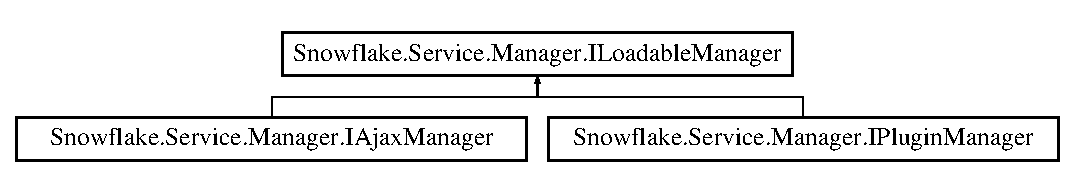
\includegraphics[height=1.924399cm]{interface_snowflake_1_1_service_1_1_manager_1_1_i_loadable_manager}
\end{center}
\end{figure}
\subsection*{Public Member Functions}
\begin{DoxyCompactItemize}
\item 
\hypertarget{interface_snowflake_1_1_service_1_1_manager_1_1_i_loadable_manager_a6b9d4f63d104f22054e0a54c4a98e667}{}void {\bfseries Load\+All} ()\label{interface_snowflake_1_1_service_1_1_manager_1_1_i_loadable_manager_a6b9d4f63d104f22054e0a54c4a98e667}

\end{DoxyCompactItemize}
\subsection*{Properties}
\begin{DoxyCompactItemize}
\item 
\hypertarget{interface_snowflake_1_1_service_1_1_manager_1_1_i_loadable_manager_aa13ef1f4fce3acadd876850e3da3c07c}{}I\+Read\+Only\+Dictionary$<$ string, Type $>$ {\bfseries Registry}\hspace{0.3cm}{\ttfamily  \mbox{[}get\mbox{]}}\label{interface_snowflake_1_1_service_1_1_manager_1_1_i_loadable_manager_aa13ef1f4fce3acadd876850e3da3c07c}

\item 
\hypertarget{interface_snowflake_1_1_service_1_1_manager_1_1_i_loadable_manager_a10c63816f664d2730455837e1484a081}{}string {\bfseries Loadables\+Location}\hspace{0.3cm}{\ttfamily  \mbox{[}get\mbox{]}}\label{interface_snowflake_1_1_service_1_1_manager_1_1_i_loadable_manager_a10c63816f664d2730455837e1484a081}

\end{DoxyCompactItemize}


The documentation for this interface was generated from the following file\+:\begin{DoxyCompactItemize}
\item 
Service/\+Manager/I\+Loadable\+Manager.\+cs\end{DoxyCompactItemize}

\hypertarget{interface_snowflake_1_1_information_1_1_media_store_1_1_i_media_store}{}\section{Snowflake.\+Information.\+Media\+Store.\+I\+Media\+Store Interface Reference}
\label{interface_snowflake_1_1_information_1_1_media_store_1_1_i_media_store}\index{Snowflake.\+Information.\+Media\+Store.\+I\+Media\+Store@{Snowflake.\+Information.\+Media\+Store.\+I\+Media\+Store}}
\subsection*{Properties}
\begin{DoxyCompactItemize}
\item 
\hypertarget{interface_snowflake_1_1_information_1_1_media_store_1_1_i_media_store_a3925774cc1ddc8c2171398ca21638569}{}\hyperlink{interface_snowflake_1_1_information_1_1_media_store_1_1_i_media_store_section}{I\+Media\+Store\+Section} {\bfseries Images}\hspace{0.3cm}{\ttfamily  \mbox{[}get\mbox{]}}\label{interface_snowflake_1_1_information_1_1_media_store_1_1_i_media_store_a3925774cc1ddc8c2171398ca21638569}

\item 
\hypertarget{interface_snowflake_1_1_information_1_1_media_store_1_1_i_media_store_a283752cbb2839696fe291e4976b435ed}{}\hyperlink{interface_snowflake_1_1_information_1_1_media_store_1_1_i_media_store_section}{I\+Media\+Store\+Section} {\bfseries Audio}\hspace{0.3cm}{\ttfamily  \mbox{[}get\mbox{]}}\label{interface_snowflake_1_1_information_1_1_media_store_1_1_i_media_store_a283752cbb2839696fe291e4976b435ed}

\item 
\hypertarget{interface_snowflake_1_1_information_1_1_media_store_1_1_i_media_store_a0d8d5f35916dad519af29f96c5015225}{}\hyperlink{interface_snowflake_1_1_information_1_1_media_store_1_1_i_media_store_section}{I\+Media\+Store\+Section} {\bfseries Video}\hspace{0.3cm}{\ttfamily  \mbox{[}get\mbox{]}}\label{interface_snowflake_1_1_information_1_1_media_store_1_1_i_media_store_a0d8d5f35916dad519af29f96c5015225}

\item 
\hypertarget{interface_snowflake_1_1_information_1_1_media_store_1_1_i_media_store_a68360d177681f9ba57362e334f71543d}{}\hyperlink{interface_snowflake_1_1_information_1_1_media_store_1_1_i_media_store_section}{I\+Media\+Store\+Section} {\bfseries Resources}\hspace{0.3cm}{\ttfamily  \mbox{[}get\mbox{]}}\label{interface_snowflake_1_1_information_1_1_media_store_1_1_i_media_store_a68360d177681f9ba57362e334f71543d}

\item 
\hypertarget{interface_snowflake_1_1_information_1_1_media_store_1_1_i_media_store_a025d3397b198dea6450ee0ca1de38d2f}{}string {\bfseries Media\+Store\+Key}\hspace{0.3cm}{\ttfamily  \mbox{[}get\mbox{]}}\label{interface_snowflake_1_1_information_1_1_media_store_1_1_i_media_store_a025d3397b198dea6450ee0ca1de38d2f}

\end{DoxyCompactItemize}


The documentation for this interface was generated from the following file\+:\begin{DoxyCompactItemize}
\item 
Information/\+Media\+Store/I\+Media\+Store.\+cs\end{DoxyCompactItemize}

\hypertarget{interface_snowflake_1_1_information_1_1_media_store_1_1_i_media_store_section}{}\section{Snowflake.\+Information.\+Media\+Store.\+I\+Media\+Store\+Section Interface Reference}
\label{interface_snowflake_1_1_information_1_1_media_store_1_1_i_media_store_section}\index{Snowflake.\+Information.\+Media\+Store.\+I\+Media\+Store\+Section@{Snowflake.\+Information.\+Media\+Store.\+I\+Media\+Store\+Section}}


Represents a section in the mediastore.  


\subsection*{Public Member Functions}
\begin{DoxyCompactItemize}
\item 
void \hyperlink{interface_snowflake_1_1_information_1_1_media_store_1_1_i_media_store_section_af3dc1bd02ecb2d3338f94651480e4b30}{Add} (string key, string value)
\begin{DoxyCompactList}\small\item\em Add a file to the mediastore \end{DoxyCompactList}\item 
void \hyperlink{interface_snowflake_1_1_information_1_1_media_store_1_1_i_media_store_section_aae9c8aa021f6477d289e1d572f7a6aeb}{Remove} (string key)
\begin{DoxyCompactList}\small\item\em Remove a file in the mediastore \end{DoxyCompactList}\end{DoxyCompactItemize}
\subsection*{Properties}
\begin{DoxyCompactItemize}
\item 
string \hyperlink{interface_snowflake_1_1_information_1_1_media_store_1_1_i_media_store_section_ab0d70ad45cbbb8aadf5cd992e6d274d4}{Section\+Name}\hspace{0.3cm}{\ttfamily  \mbox{[}get, set\mbox{]}}
\begin{DoxyCompactList}\small\item\em The name of the mediastore. \end{DoxyCompactList}\item 
I\+Read\+Only\+Dictionary$<$ string, string $>$ \hyperlink{interface_snowflake_1_1_information_1_1_media_store_1_1_i_media_store_section_ad756842e38469738145eec216952c9b5}{Media\+Store\+Items}\hspace{0.3cm}{\ttfamily  \mbox{[}get\mbox{]}}
\begin{DoxyCompactList}\small\item\em A dictionary holding all the items in the mediastore. Never access this dictionary directly, instead use the indexer. \end{DoxyCompactList}\item 
string \hyperlink{interface_snowflake_1_1_information_1_1_media_store_1_1_i_media_store_section_ad878b6801659f539a1482b12e09468f6}{this\mbox{[}string key\mbox{]}}\hspace{0.3cm}{\ttfamily  \mbox{[}get, set\mbox{]}}
\begin{DoxyCompactList}\small\item\em Access a certain item in the mediastore \end{DoxyCompactList}\end{DoxyCompactItemize}


\subsection{Detailed Description}
Represents a section in the mediastore. 



\subsection{Member Function Documentation}
\hypertarget{interface_snowflake_1_1_information_1_1_media_store_1_1_i_media_store_section_af3dc1bd02ecb2d3338f94651480e4b30}{}\index{Snowflake\+::\+Information\+::\+Media\+Store\+::\+I\+Media\+Store\+Section@{Snowflake\+::\+Information\+::\+Media\+Store\+::\+I\+Media\+Store\+Section}!Add@{Add}}
\index{Add@{Add}!Snowflake\+::\+Information\+::\+Media\+Store\+::\+I\+Media\+Store\+Section@{Snowflake\+::\+Information\+::\+Media\+Store\+::\+I\+Media\+Store\+Section}}
\subsubsection[{Add}]{\setlength{\rightskip}{0pt plus 5cm}void Snowflake.\+Information.\+Media\+Store.\+I\+Media\+Store\+Section.\+Add (
\begin{DoxyParamCaption}
\item[{string}]{key, }
\item[{string}]{value}
\end{DoxyParamCaption}
)}\label{interface_snowflake_1_1_information_1_1_media_store_1_1_i_media_store_section_af3dc1bd02ecb2d3338f94651480e4b30}


Add a file to the mediastore 


\begin{DoxyParams}{Parameters}
{\em key} & The key in which to store the item\\
\hline
{\em value} & The path to the file to be added\\
\hline
\end{DoxyParams}
\hypertarget{interface_snowflake_1_1_information_1_1_media_store_1_1_i_media_store_section_aae9c8aa021f6477d289e1d572f7a6aeb}{}\index{Snowflake\+::\+Information\+::\+Media\+Store\+::\+I\+Media\+Store\+Section@{Snowflake\+::\+Information\+::\+Media\+Store\+::\+I\+Media\+Store\+Section}!Remove@{Remove}}
\index{Remove@{Remove}!Snowflake\+::\+Information\+::\+Media\+Store\+::\+I\+Media\+Store\+Section@{Snowflake\+::\+Information\+::\+Media\+Store\+::\+I\+Media\+Store\+Section}}
\subsubsection[{Remove}]{\setlength{\rightskip}{0pt plus 5cm}void Snowflake.\+Information.\+Media\+Store.\+I\+Media\+Store\+Section.\+Remove (
\begin{DoxyParamCaption}
\item[{string}]{key}
\end{DoxyParamCaption}
)}\label{interface_snowflake_1_1_information_1_1_media_store_1_1_i_media_store_section_aae9c8aa021f6477d289e1d572f7a6aeb}


Remove a file in the mediastore 


\begin{DoxyParams}{Parameters}
{\em key} & The key of the mediastore item\\
\hline
\end{DoxyParams}


\subsection{Property Documentation}
\hypertarget{interface_snowflake_1_1_information_1_1_media_store_1_1_i_media_store_section_ad756842e38469738145eec216952c9b5}{}\index{Snowflake\+::\+Information\+::\+Media\+Store\+::\+I\+Media\+Store\+Section@{Snowflake\+::\+Information\+::\+Media\+Store\+::\+I\+Media\+Store\+Section}!Media\+Store\+Items@{Media\+Store\+Items}}
\index{Media\+Store\+Items@{Media\+Store\+Items}!Snowflake\+::\+Information\+::\+Media\+Store\+::\+I\+Media\+Store\+Section@{Snowflake\+::\+Information\+::\+Media\+Store\+::\+I\+Media\+Store\+Section}}
\subsubsection[{Media\+Store\+Items}]{\setlength{\rightskip}{0pt plus 5cm}I\+Read\+Only\+Dictionary$<$string, string$>$ Snowflake.\+Information.\+Media\+Store.\+I\+Media\+Store\+Section.\+Media\+Store\+Items\hspace{0.3cm}{\ttfamily [get]}}\label{interface_snowflake_1_1_information_1_1_media_store_1_1_i_media_store_section_ad756842e38469738145eec216952c9b5}


A dictionary holding all the items in the mediastore. Never access this dictionary directly, instead use the indexer. 

\hypertarget{interface_snowflake_1_1_information_1_1_media_store_1_1_i_media_store_section_ab0d70ad45cbbb8aadf5cd992e6d274d4}{}\index{Snowflake\+::\+Information\+::\+Media\+Store\+::\+I\+Media\+Store\+Section@{Snowflake\+::\+Information\+::\+Media\+Store\+::\+I\+Media\+Store\+Section}!Section\+Name@{Section\+Name}}
\index{Section\+Name@{Section\+Name}!Snowflake\+::\+Information\+::\+Media\+Store\+::\+I\+Media\+Store\+Section@{Snowflake\+::\+Information\+::\+Media\+Store\+::\+I\+Media\+Store\+Section}}
\subsubsection[{Section\+Name}]{\setlength{\rightskip}{0pt plus 5cm}string Snowflake.\+Information.\+Media\+Store.\+I\+Media\+Store\+Section.\+Section\+Name\hspace{0.3cm}{\ttfamily [get]}, {\ttfamily [set]}}\label{interface_snowflake_1_1_information_1_1_media_store_1_1_i_media_store_section_ab0d70ad45cbbb8aadf5cd992e6d274d4}


The name of the mediastore. 

\hypertarget{interface_snowflake_1_1_information_1_1_media_store_1_1_i_media_store_section_ad878b6801659f539a1482b12e09468f6}{}\index{Snowflake\+::\+Information\+::\+Media\+Store\+::\+I\+Media\+Store\+Section@{Snowflake\+::\+Information\+::\+Media\+Store\+::\+I\+Media\+Store\+Section}!this\mbox{[}string key\mbox{]}@{this[string key]}}
\index{this\mbox{[}string key\mbox{]}@{this[string key]}!Snowflake\+::\+Information\+::\+Media\+Store\+::\+I\+Media\+Store\+Section@{Snowflake\+::\+Information\+::\+Media\+Store\+::\+I\+Media\+Store\+Section}}
\subsubsection[{this[string key]}]{\setlength{\rightskip}{0pt plus 5cm}string Snowflake.\+Information.\+Media\+Store.\+I\+Media\+Store\+Section.\+this\mbox{[}string key\mbox{]}\hspace{0.3cm}{\ttfamily [get]}, {\ttfamily [set]}}\label{interface_snowflake_1_1_information_1_1_media_store_1_1_i_media_store_section_ad878b6801659f539a1482b12e09468f6}


Access a certain item in the mediastore 


\begin{DoxyParams}{Parameters}
{\em key} & The key of the mediastore item\\
\hline
\end{DoxyParams}
\begin{DoxyReturn}{Returns}
The path to the mediastore item
\end{DoxyReturn}


The documentation for this interface was generated from the following file\+:\begin{DoxyCompactItemize}
\item 
Information/\+Media\+Store/I\+Media\+Store\+Section.\+cs\end{DoxyCompactItemize}

\hypertarget{interface_snowflake_1_1_platform_1_1_i_platform_defaults}{}\section{Snowflake.\+Platform.\+I\+Platform\+Defaults Interface Reference}
\label{interface_snowflake_1_1_platform_1_1_i_platform_defaults}\index{Snowflake.\+Platform.\+I\+Platform\+Defaults@{Snowflake.\+Platform.\+I\+Platform\+Defaults}}
\subsection*{Properties}
\begin{DoxyCompactItemize}
\item 
\hypertarget{interface_snowflake_1_1_platform_1_1_i_platform_defaults_abd3603b74dd041c42762d9d76e872a77}{}string {\bfseries Emulator}\hspace{0.3cm}{\ttfamily  \mbox{[}get, set\mbox{]}}\label{interface_snowflake_1_1_platform_1_1_i_platform_defaults_abd3603b74dd041c42762d9d76e872a77}

\item 
\hypertarget{interface_snowflake_1_1_platform_1_1_i_platform_defaults_abdf4bdbce92fd8e6426b6f893d22457b}{}string {\bfseries Identifier}\hspace{0.3cm}{\ttfamily  \mbox{[}get, set\mbox{]}}\label{interface_snowflake_1_1_platform_1_1_i_platform_defaults_abdf4bdbce92fd8e6426b6f893d22457b}

\item 
\hypertarget{interface_snowflake_1_1_platform_1_1_i_platform_defaults_a5d3e39d4443a13e6ce452efbd409afb0}{}string {\bfseries Scraper}\hspace{0.3cm}{\ttfamily  \mbox{[}get, set\mbox{]}}\label{interface_snowflake_1_1_platform_1_1_i_platform_defaults_a5d3e39d4443a13e6ce452efbd409afb0}

\end{DoxyCompactItemize}


The documentation for this interface was generated from the following file\+:\begin{DoxyCompactItemize}
\item 
Platform/I\+Platform\+Defaults.\+cs\end{DoxyCompactItemize}

\hypertarget{interface_snowflake_1_1_platform_1_1_i_platform_info}{}\section{Snowflake.\+Platform.\+I\+Platform\+Info Interface Reference}
\label{interface_snowflake_1_1_platform_1_1_i_platform_info}\index{Snowflake.\+Platform.\+I\+Platform\+Info@{Snowflake.\+Platform.\+I\+Platform\+Info}}


Represents an emulated console or a platform in \hyperlink{namespace_snowflake}{Snowflake}.  


Inheritance diagram for Snowflake.\+Platform.\+I\+Platform\+Info\+:\begin{figure}[H]
\begin{center}
\leavevmode
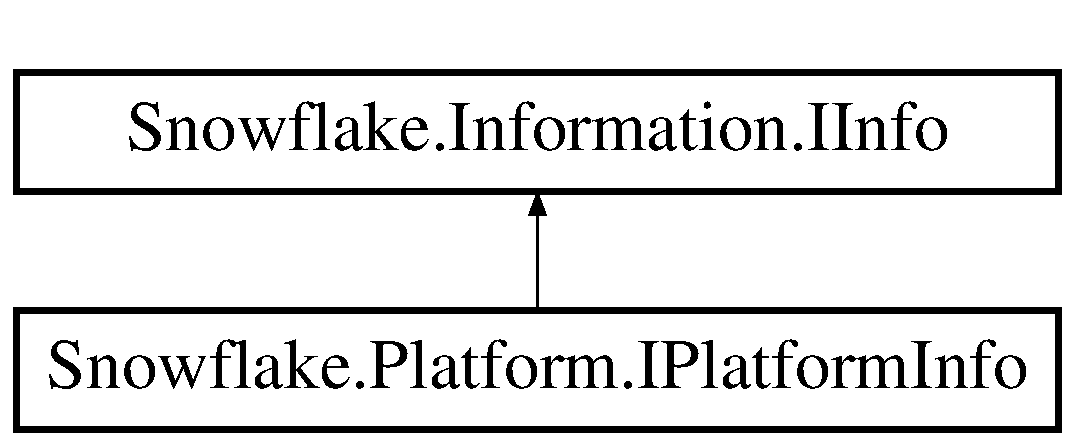
\includegraphics[height=2.000000cm]{interface_snowflake_1_1_platform_1_1_i_platform_info}
\end{center}
\end{figure}
\subsection*{Properties}
\begin{DoxyCompactItemize}
\item 
I\+Read\+Only\+Dictionary$<$ string, \hyperlink{interface_snowflake_1_1_controller_1_1_i_controller_definition}{I\+Controller\+Definition} $>$ \hyperlink{interface_snowflake_1_1_platform_1_1_i_platform_info_a1151f29fd2b955e694257a3ea83b19eb}{Controllers}\hspace{0.3cm}{\ttfamily  \mbox{[}get\mbox{]}}
\begin{DoxyCompactList}\small\item\em The controllers in a platform. \end{DoxyCompactList}\item 
\hypertarget{interface_snowflake_1_1_platform_1_1_i_platform_info_a0ce0061b2706d418974f14552cf33f38}{}\hyperlink{interface_snowflake_1_1_platform_1_1_i_platform_defaults}{I\+Platform\+Defaults} {\bfseries Defaults}\hspace{0.3cm}{\ttfamily  \mbox{[}get, set\mbox{]}}\label{interface_snowflake_1_1_platform_1_1_i_platform_info_a0ce0061b2706d418974f14552cf33f38}

\item 
I\+List$<$ string $>$ \hyperlink{interface_snowflake_1_1_platform_1_1_i_platform_info_a2e12201a96a5804f7f97dc3239d6a4d3}{File\+Extensions}\hspace{0.3cm}{\ttfamily  \mbox{[}get\mbox{]}}
\begin{DoxyCompactList}\small\item\em The file extensions R\+O\+Ms of this platform are known to have. \end{DoxyCompactList}\item 
int \hyperlink{interface_snowflake_1_1_platform_1_1_i_platform_info_a3d087c38d145982e8fb26d5adbaaf545}{Maximum\+Inputs}\hspace{0.3cm}{\ttfamily  \mbox{[}get\mbox{]}}
\begin{DoxyCompactList}\small\item\em The maximum amount of inputs that are physically possible for this platform to have. \end{DoxyCompactList}\end{DoxyCompactItemize}


\subsection{Detailed Description}
Represents an emulated console or a platform in \hyperlink{namespace_snowflake}{Snowflake}. 



\subsection{Property Documentation}
\hypertarget{interface_snowflake_1_1_platform_1_1_i_platform_info_a1151f29fd2b955e694257a3ea83b19eb}{}\index{Snowflake\+::\+Platform\+::\+I\+Platform\+Info@{Snowflake\+::\+Platform\+::\+I\+Platform\+Info}!Controllers@{Controllers}}
\index{Controllers@{Controllers}!Snowflake\+::\+Platform\+::\+I\+Platform\+Info@{Snowflake\+::\+Platform\+::\+I\+Platform\+Info}}
\subsubsection[{Controllers}]{\setlength{\rightskip}{0pt plus 5cm}I\+Read\+Only\+Dictionary$<$string, {\bf I\+Controller\+Definition}$>$ Snowflake.\+Platform.\+I\+Platform\+Info.\+Controllers\hspace{0.3cm}{\ttfamily [get]}}\label{interface_snowflake_1_1_platform_1_1_i_platform_info_a1151f29fd2b955e694257a3ea83b19eb}


The controllers in a platform. 

\hypertarget{interface_snowflake_1_1_platform_1_1_i_platform_info_a2e12201a96a5804f7f97dc3239d6a4d3}{}\index{Snowflake\+::\+Platform\+::\+I\+Platform\+Info@{Snowflake\+::\+Platform\+::\+I\+Platform\+Info}!File\+Extensions@{File\+Extensions}}
\index{File\+Extensions@{File\+Extensions}!Snowflake\+::\+Platform\+::\+I\+Platform\+Info@{Snowflake\+::\+Platform\+::\+I\+Platform\+Info}}
\subsubsection[{File\+Extensions}]{\setlength{\rightskip}{0pt plus 5cm}I\+List$<$string$>$ Snowflake.\+Platform.\+I\+Platform\+Info.\+File\+Extensions\hspace{0.3cm}{\ttfamily [get]}}\label{interface_snowflake_1_1_platform_1_1_i_platform_info_a2e12201a96a5804f7f97dc3239d6a4d3}


The file extensions R\+O\+Ms of this platform are known to have. 

\hypertarget{interface_snowflake_1_1_platform_1_1_i_platform_info_a3d087c38d145982e8fb26d5adbaaf545}{}\index{Snowflake\+::\+Platform\+::\+I\+Platform\+Info@{Snowflake\+::\+Platform\+::\+I\+Platform\+Info}!Maximum\+Inputs@{Maximum\+Inputs}}
\index{Maximum\+Inputs@{Maximum\+Inputs}!Snowflake\+::\+Platform\+::\+I\+Platform\+Info@{Snowflake\+::\+Platform\+::\+I\+Platform\+Info}}
\subsubsection[{Maximum\+Inputs}]{\setlength{\rightskip}{0pt plus 5cm}int Snowflake.\+Platform.\+I\+Platform\+Info.\+Maximum\+Inputs\hspace{0.3cm}{\ttfamily [get]}}\label{interface_snowflake_1_1_platform_1_1_i_platform_info_a3d087c38d145982e8fb26d5adbaaf545}


The maximum amount of inputs that are physically possible for this platform to have. 



The documentation for this interface was generated from the following file\+:\begin{DoxyCompactItemize}
\item 
Platform/I\+Platform\+Info.\+cs\end{DoxyCompactItemize}

\hypertarget{interface_snowflake_1_1_plugin_1_1_i_plugin_configuration}{}\section{Snowflake.\+Plugin.\+I\+Plugin\+Configuration Interface Reference}
\label{interface_snowflake_1_1_plugin_1_1_i_plugin_configuration}\index{Snowflake.\+Plugin.\+I\+Plugin\+Configuration@{Snowflake.\+Plugin.\+I\+Plugin\+Configuration}}
\subsection*{Public Member Functions}
\begin{DoxyCompactItemize}
\item 
\hypertarget{interface_snowflake_1_1_plugin_1_1_i_plugin_configuration_a41c815380eabd81bae7e678da5b04884}{}void {\bfseries Load\+Configuration} ()\label{interface_snowflake_1_1_plugin_1_1_i_plugin_configuration_a41c815380eabd81bae7e678da5b04884}

\item 
\hypertarget{interface_snowflake_1_1_plugin_1_1_i_plugin_configuration_a22f475e74370ce7c609a9c8ce6c3a9dd}{}void {\bfseries Save\+Configuration} ()\label{interface_snowflake_1_1_plugin_1_1_i_plugin_configuration_a22f475e74370ce7c609a9c8ce6c3a9dd}

\end{DoxyCompactItemize}
\subsection*{Properties}
\begin{DoxyCompactItemize}
\item 
\hypertarget{interface_snowflake_1_1_plugin_1_1_i_plugin_configuration_a7f457d870f0808d2ef41866df200e008}{}string {\bfseries Configuration\+File\+Name}\hspace{0.3cm}{\ttfamily  \mbox{[}get\mbox{]}}\label{interface_snowflake_1_1_plugin_1_1_i_plugin_configuration_a7f457d870f0808d2ef41866df200e008}

\item 
\hypertarget{interface_snowflake_1_1_plugin_1_1_i_plugin_configuration_a7cfa77237b6d1785e8f8b1a0eed3ddf8}{}I\+Dictionary$<$ string, dynamic $>$ {\bfseries Configuration}\hspace{0.3cm}{\ttfamily  \mbox{[}get\mbox{]}}\label{interface_snowflake_1_1_plugin_1_1_i_plugin_configuration_a7cfa77237b6d1785e8f8b1a0eed3ddf8}

\end{DoxyCompactItemize}


The documentation for this interface was generated from the following file\+:\begin{DoxyCompactItemize}
\item 
Plugin/I\+Plugin\+Configuration.\+cs\end{DoxyCompactItemize}

\hypertarget{interface_snowflake_1_1_service_1_1_manager_1_1_i_plugin_manager}{}\section{Snowflake.\+Service.\+Manager.\+I\+Plugin\+Manager Interface Reference}
\label{interface_snowflake_1_1_service_1_1_manager_1_1_i_plugin_manager}\index{Snowflake.\+Service.\+Manager.\+I\+Plugin\+Manager@{Snowflake.\+Service.\+Manager.\+I\+Plugin\+Manager}}
Inheritance diagram for Snowflake.\+Service.\+Manager.\+I\+Plugin\+Manager\+:\begin{figure}[H]
\begin{center}
\leavevmode
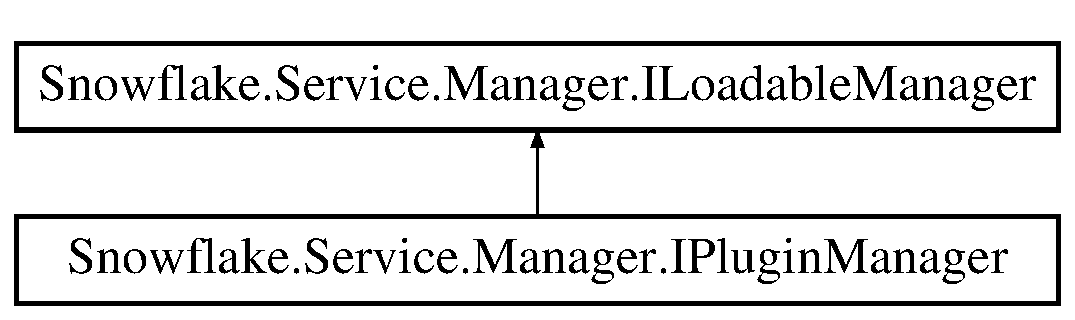
\includegraphics[height=2.000000cm]{interface_snowflake_1_1_service_1_1_manager_1_1_i_plugin_manager}
\end{center}
\end{figure}
\subsection*{Properties}
\begin{DoxyCompactItemize}
\item 
\hypertarget{interface_snowflake_1_1_service_1_1_manager_1_1_i_plugin_manager_a0289061b9332b8fc82aadc61438c3149}{}I\+Read\+Only\+Dictionary$<$ string, \hyperlink{interface_snowflake_1_1_emulator_1_1_i_emulator_bridge}{I\+Emulator\+Bridge} $>$ {\bfseries Loaded\+Emulators}\hspace{0.3cm}{\ttfamily  \mbox{[}get\mbox{]}}\label{interface_snowflake_1_1_service_1_1_manager_1_1_i_plugin_manager_a0289061b9332b8fc82aadc61438c3149}

\item 
\hypertarget{interface_snowflake_1_1_service_1_1_manager_1_1_i_plugin_manager_a01aab2cca52df8cd34162458b6cbd276}{}I\+Read\+Only\+Dictionary$<$ string, \hyperlink{interface_snowflake_1_1_identifier_1_1_i_identifier}{I\+Identifier} $>$ {\bfseries Loaded\+Identifiers}\hspace{0.3cm}{\ttfamily  \mbox{[}get\mbox{]}}\label{interface_snowflake_1_1_service_1_1_manager_1_1_i_plugin_manager_a01aab2cca52df8cd34162458b6cbd276}

\item 
\hypertarget{interface_snowflake_1_1_service_1_1_manager_1_1_i_plugin_manager_a13b43ef53ea5bd28b624884f4e19db5d}{}I\+Read\+Only\+Dictionary$<$ string, \hyperlink{interface_snowflake_1_1_plugin_1_1_i_general_plugin}{I\+General\+Plugin} $>$ {\bfseries Loaded\+Plugins}\hspace{0.3cm}{\ttfamily  \mbox{[}get\mbox{]}}\label{interface_snowflake_1_1_service_1_1_manager_1_1_i_plugin_manager_a13b43ef53ea5bd28b624884f4e19db5d}

\item 
\hypertarget{interface_snowflake_1_1_service_1_1_manager_1_1_i_plugin_manager_a94bad112601b36f9c9b54c556d870490}{}I\+Read\+Only\+Dictionary$<$ string, \hyperlink{interface_snowflake_1_1_scraper_1_1_i_scraper}{I\+Scraper} $>$ {\bfseries Loaded\+Scrapers}\hspace{0.3cm}{\ttfamily  \mbox{[}get\mbox{]}}\label{interface_snowflake_1_1_service_1_1_manager_1_1_i_plugin_manager_a94bad112601b36f9c9b54c556d870490}

\end{DoxyCompactItemize}
\subsection*{Additional Inherited Members}


The documentation for this interface was generated from the following file\+:\begin{DoxyCompactItemize}
\item 
Service/\+Manager/I\+Plugin\+Manager.\+cs\end{DoxyCompactItemize}

\hypertarget{interface_snowflake_1_1_scraper_1_1_i_scraper}{}\section{Snowflake.\+Scraper.\+I\+Scraper Interface Reference}
\label{interface_snowflake_1_1_scraper_1_1_i_scraper}\index{Snowflake.\+Scraper.\+I\+Scraper@{Snowflake.\+Scraper.\+I\+Scraper}}
Inheritance diagram for Snowflake.\+Scraper.\+I\+Scraper\+:\begin{figure}[H]
\begin{center}
\leavevmode
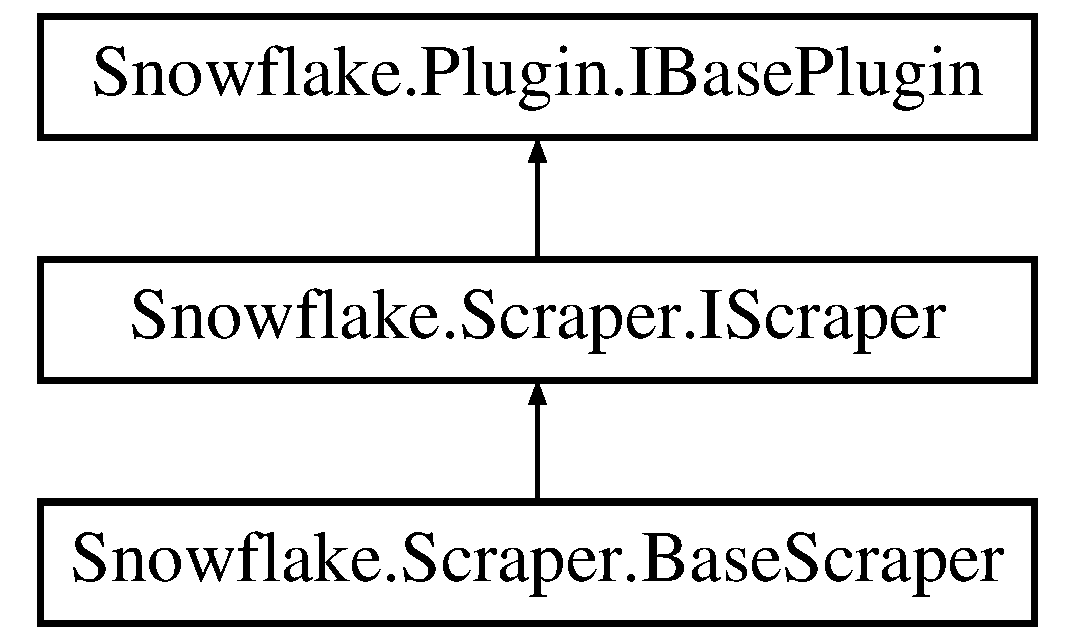
\includegraphics[height=3.000000cm]{interface_snowflake_1_1_scraper_1_1_i_scraper}
\end{center}
\end{figure}
\subsection*{Public Member Functions}
\begin{DoxyCompactItemize}
\item 
\hypertarget{interface_snowflake_1_1_scraper_1_1_i_scraper_a133e1a55dd154335843993d3f1166db3}{}I\+List$<$ \hyperlink{interface_snowflake_1_1_scraper_1_1_i_game_scrape_result}{I\+Game\+Scrape\+Result} $>$ {\bfseries Get\+Search\+Results} (string search\+Query)\label{interface_snowflake_1_1_scraper_1_1_i_scraper_a133e1a55dd154335843993d3f1166db3}

\item 
\hypertarget{interface_snowflake_1_1_scraper_1_1_i_scraper_aa72dd3d46e143253c31b8b99b9f2fb23}{}I\+List$<$ \hyperlink{interface_snowflake_1_1_scraper_1_1_i_game_scrape_result}{I\+Game\+Scrape\+Result} $>$ {\bfseries Get\+Search\+Results} (string search\+Query, string platform\+Id)\label{interface_snowflake_1_1_scraper_1_1_i_scraper_aa72dd3d46e143253c31b8b99b9f2fb23}

\item 
\hypertarget{interface_snowflake_1_1_scraper_1_1_i_scraper_a2ce05496e052fbb3b3e478813d7d6075}{}Tuple$<$ I\+Dictionary$<$ string, string $>$, \hyperlink{interface_snowflake_1_1_scraper_1_1_i_game_images_result}{I\+Game\+Images\+Result} $>$ {\bfseries Get\+Game\+Details} (string id)\label{interface_snowflake_1_1_scraper_1_1_i_scraper_a2ce05496e052fbb3b3e478813d7d6075}

\end{DoxyCompactItemize}
\subsection*{Properties}
\begin{DoxyCompactItemize}
\item 
\hypertarget{interface_snowflake_1_1_scraper_1_1_i_scraper_a5b576c3bf032e77c6de722139b98cc15}{}\hyperlink{class_snowflake_1_1_utility_1_1_bi_dictionary}{Bi\+Dictionary}$<$ string, string $>$ {\bfseries Scraper\+Map}\hspace{0.3cm}{\ttfamily  \mbox{[}get\mbox{]}}\label{interface_snowflake_1_1_scraper_1_1_i_scraper_a5b576c3bf032e77c6de722139b98cc15}

\end{DoxyCompactItemize}


The documentation for this interface was generated from the following file\+:\begin{DoxyCompactItemize}
\item 
Scraper/I\+Scraper.\+cs\end{DoxyCompactItemize}

\hypertarget{interface_snowflake_1_1_service_1_1_i_scrape_service}{}\section{Snowflake.\+Service.\+I\+Scrape\+Service Interface Reference}
\label{interface_snowflake_1_1_service_1_1_i_scrape_service}\index{Snowflake.\+Service.\+I\+Scrape\+Service@{Snowflake.\+Service.\+I\+Scrape\+Service}}
\subsection*{Public Member Functions}
\begin{DoxyCompactItemize}
\item 
\hypertarget{interface_snowflake_1_1_service_1_1_i_scrape_service_a75fc36352cf276850467a502cd9a938d}{}\hyperlink{interface_snowflake_1_1_game_1_1_i_game_info}{I\+Game\+Info} {\bfseries Get\+Game\+Info} (string file\+Name)\label{interface_snowflake_1_1_service_1_1_i_scrape_service_a75fc36352cf276850467a502cd9a938d}

\end{DoxyCompactItemize}


The documentation for this interface was generated from the following file\+:\begin{DoxyCompactItemize}
\item 
Service/I\+Scrape\+Service.\+cs\end{DoxyCompactItemize}

\hypertarget{class_snowflake_1_1_events_1_1_core_events_1_1_plugin_manager_loaded_event_args}{}\section{Snowflake.\+Events.\+Core\+Events.\+Plugin\+Manager\+Loaded\+Event\+Args Class Reference}
\label{class_snowflake_1_1_events_1_1_core_events_1_1_plugin_manager_loaded_event_args}\index{Snowflake.\+Events.\+Core\+Events.\+Plugin\+Manager\+Loaded\+Event\+Args@{Snowflake.\+Events.\+Core\+Events.\+Plugin\+Manager\+Loaded\+Event\+Args}}
Inheritance diagram for Snowflake.\+Events.\+Core\+Events.\+Plugin\+Manager\+Loaded\+Event\+Args\+:\begin{figure}[H]
\begin{center}
\leavevmode
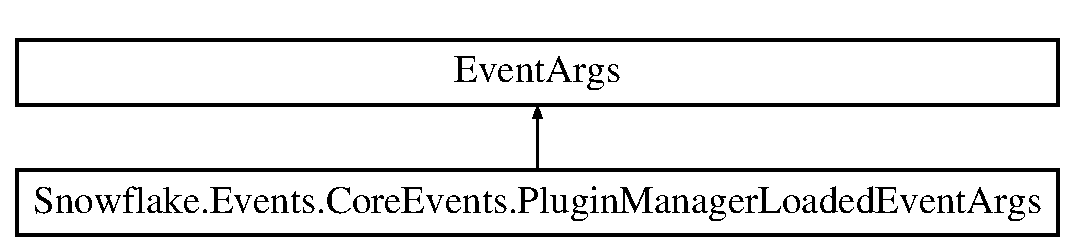
\includegraphics[height=2.000000cm]{class_snowflake_1_1_events_1_1_core_events_1_1_plugin_manager_loaded_event_args}
\end{center}
\end{figure}


The documentation for this class was generated from the following file\+:\begin{DoxyCompactItemize}
\item 
Events/Plugin\+Manager\+Loaded\+Event\+Args.\+cs\end{DoxyCompactItemize}

%--- End generated contents ---

% Index
\backmatter
\newpage
\phantomsection
\clearemptydoublepage
\addcontentsline{toc}{chapter}{Index}
\printindex

\end{document}
